% Newest hyphenation (put it in front of documentclass)
 \RequirePackage[english=usenglish]{hyphsubst}
%\RequirePackage[ngerman=ngerman-x-latest]{hyphsubst}

\documentclass[
    %ngerman, % 
    english,
    a4paper,
    12pt,
    twoside, % twoside
    final,
    numbers=noenddot, % Avoid i.e. "5.5." for chapters, write "5.5"
    toc=bibliography,
    toc=listof
]{scrbook}


% % % % Language and encoding

% Allow the complete utf8 character set. Be careful so save all files in utf8 encoding. This is especially important for German umlauts.
\usepackage[utf8]{inputenc}
\usepackage{babel}


% % % % Page layout related features

% Alternative to the fancyhdr-package which fits better to scrbook since both are part of KOMA-script, the following style is partly defined by Joerg
\usepackage{scrpage2}
\pagestyle{scrheadings}
\clearscrheadfoot
\renewcommand{\chaptermark}[1]{\markboth{#1}{}}
\renewcommand{\sectionmark}[1]{\markright{-~#1}{}}
\ihead{\leftmark}
\chead{}
\ofoot{}
\setheadsepline{.4pt}
\cfoot[\pagemark]{}
\ohead[]{\pagemark}

% Disables header and footer in italic
\setkomafont{pageheadfoot}{\normalfont}

% Package to create horizontal rules around chapter titles
\usepackage{titlesec}

% Page size definition by original author
\setlength{\oddsidemargin}{5mm}
\setlength{\evensidemargin}{0mm}
\setlength{\textwidth}{155mm}
\setlength{\topmargin}{-5mm}
\setlength{\textheight}{235mm}


% % % % Text layout related features

% Subliminal refinements towards typographical perfection
\usepackage{microtype}

\usepackage{xspace}
\usepackage{rotating}

% It provides \textcolor{<color>}{<text>} as well as \color{<color>} to switch the color for some give text or until the end of the group/environment. You can get different shades of gray by using black!x as a color where x is a number from 0 to 100, taken as a percentage.
\usepackage{xcolor}
\newcommand{\inred}[1]{\xspace{\color{red} #1}\xspace} % Use this command to make annotations, which will be removed in the final document.

% Allow URLs to break at hyphens
\usepackage[hyphens]{url}

% Change style to the style of the normal text instead of ttfamily style.
\urlstyle{same}

% Do not indent the beginning of a new paragraph
\usepackage[parfill]{parskip}


% % % % Math related features

% The bm package is loaded, but you should still use \mathbf and \boldsymbol to remain compatible with MathJax.
\usepackage{amssymb, amsmath, bm}


% This package is the current package for units and outperforms siunits and similar packages
%\usepackage[decimalsymbol=comma, expproduct=times]{siunitx} % German notation
\usepackage[expproduct=times]{siunitx} % American notation


% % % % Source code related features

% Put in source code into your document, this especially allows inline source code with \lstinline!example!, where "!" can be exchanged by any delimiter
\usepackage{listings}
\lstset{
    basicstyle=\ttfamily
}

% Pseudo code
\usepackage{algorithm}
\usepackage{algpseudocode}
% Allow one-line if conditions
\newcommand{\LineIf}[3]{ \State \algorithmicif\ {#1}\ \algorithmicthen\ {#2} \algorithmicend\ \algorithmicif }


% % % % Image and plot related features
\graphicspath{{eps/}}							% Festlegung des Pfades zu den Bildern
\DeclareGraphicsExtensions{.eps}
% Use TikZ to draw images
\usepackage{pgfplots} % Import der Plots aus Matlab
\newlength\fheight % Plots aus Matlab immer gleich gross
\newlength\fwidth % Plots aus Matlab immer gleich gross
\usepackage{tikz}
\pgfplotsset{compat=1.9}

% Precompile TikZ pictures for speedup, this does not seem to work in Poolroom yet
\usetikzlibrary{external}
% \tikzexternalize % Activate, works only with pdflatex

% Subfigure is deprecaded and subfig is the new version of subfigure
% Subcaption works with hyperref whereas subfigure is reported to be broken
\usepackage{caption}
\usepackage{subcaption}

% Use this package to import Inkscape generated pdfs with pdf_tex files
\usepackage{import}

% Macros to adjust position text in Inkscape files. Place the anchor exactly in the middle of the position where the text should appear
% Use \adjTxtPos{multiline\\text}
% or \adjTxtPosRot{lorem\\ipsum}
\newlength{\myheight}
\newcommand{\adjTxtPos}[1]{\settoheight{\myheight}{Fg}{\parbox[c]{\textheight}{\centering \vspace{\myheight}\phantom{F} #1 \\ \phantom{g} }}}
\newcommand{\adjTxtPosRot}[1]{\begin{rotate}{90}\hspace{-0.5\textheight}\adjTxtPos{#1}\end{rotate}}

% % % % Table related features

% Define new column types to allow centering and width of each cell
\usepackage{array}
\newcolumntype{L}[1]{>{\raggedright\let\newline\\\arraybackslash\hspace{0pt}}m{#1}}
\newcolumntype{C}[1]{>{\centering\let\newline\\\arraybackslash\hspace{0pt}}m{#1}}
\newcolumntype{R}[1]{>{\raggedleft\let\newline\\\arraybackslash\hspace{0pt}}m{#1}}

% Tables according to Chicago Manual of Style
\usepackage{tabularx, etoolbox, booktabs}
\usepackage{multirow} % Allows rowspan
\newcommand{\rarray}[1]{\renewcommand{\arraystretch}{#1}} % Slightly enlarged cells
\captionsetup{belowskip=12pt,aboveskip=4pt} % Correct table caption distance


% % % % Links and references setup

\usepackage{csquotes} % texdoc biblatex: If this package is available, biblatex will use its language sensitive quotation facilities to enclose certain titles in quotation marks.
\usepackage[backend=bibtex, style=alphabetic, firstinits=true]{biblatex}
% \usepackage[backend=biber, style=ieee]{biblatex} % Alternative
\setlength\bibitemsep{\baselineskip} % Custom MAWK, add space between entries
\bibliography{references}

% According to the glossaries manual, this package should be loaded after hyperref, the toc option makes the glossaries appear in the table of contents
\usepackage[acronym, toc, nonumberlist]{glossaries}
\renewcommand*{\glsgroupskip}{}
\newacronym{pmsm}{PMSM}{permanent magnet synchronous motor}

\newacronym{fea}{FEA}{Finite-Element Analysis}
\newacronym{cfd}{CFD}{Computational Fluid Dynamics}
\newacronym{lptn}{LPTN}{lumped-parameter thermal network}

\newacronym{hmm}{HMM}{hidden Markov model}

\newacronym{mlp}{MLP}{Multi Layer Perceptron}
\newacronym{ann}{ANN}{artificial neural network}
\newacronym{dnn}{DNN}{deep neural network}
\newacronym{fnn}{FNN}{feedforward neural network}
\newacronym{rnn}{RNN}{recurrent neural network}
\newacronym{brnn}{BRNN}{bidirectional recurrent neural network}
\newacronym{bptt}{BPTT}{backpropagation through time}
\newacronym[longplural={Long Short-Term Memories}]{lstm}{LSTM}{Long Short-Term Memory}
\newacronym[longplural={bidirectional Long Short-Term Memories}]{blstm}{BLSTM}{bidirectional Long Short-Term Memory}
\newacronym[longplural={general Long Short-Term Memories}]{lstmg}{LSTM-g}{General Long Short-Term Memory}
\newacronym{tdnn}{TDNN}{time-delay neural network}
\newacronym{narx}{NARX}{nonlinear autoregressive exogenous model}
\newacronym{cnn}{CNN}{convolutional neural network}
\newacronym{ntm}{NTM}{neural Turing machine}
\newacronym{gru}{GRU}{gated recurrent unit}

\newacronym{relu}{ReLU}{rectified linear unit}

\newacronym{lm}{LM}{Levenberg-Marquardt}
\newacronym{mse}{MSE}{mean squared error}
\newacronym{sgd}{SGD}{stochastic gradient descent}
\newacronym{nag}{NAG}{Nesterov accelerated gradient}
\newacronym{adam}{Adam}{adaptive moment estimation}


\newacronym{pca}{PCA}{principal component analysis}

\newacronym{psms}{PSMS}{particle swarm model selection}
\newacronym{pso}{PSO}{particle swarm optimization}

\newacronym{pc2}{PC\textsuperscript{2}}{Paderborn Center for Parallel Computing}


% Add this after all new glossary entries
\makeglossaries

% Allow URLs and other links to be clickable
% Removes borders according to: texdoc hyperref page 4
\usepackage[colorlinks=false, pdfborder={0 0 0}]{hyperref}

\DeclareMathOperator{\expontential}{exp}
\DeclareMathOperator{\trace}{tr}
\DeclareMathOperator{\argmax}{argmax}
\DeclareMathOperator{\argmin}{argmin}
\DeclareMathOperator{\variance}{var}
\DeclareMathOperator{\E}{\mathbb{E}}
\newcommand{\dif}{\mathrm{d}}

% This definition avoids two points at the end of an equation when closing equations with a full stop
\makeatletter
\newcommand{\const}{\mathrm{const}\@ifnextchar.{}{.}}
\makeatother

\newcommand{\Mytyp}{Masterthesis}
\newcommand{\Mytitel}{Investigation of Artificial Neural Networks to Estimate Important Component Temperatures Inside Permanent Magnet Synchronous Motors}
\newcommand{\Mytitelpdf}{Investigation of Artificial Neural Networks to Estimate Important Component Temperatures Inside Permanent Magnet Synchronous Motors}
\newcommand{\Myautor}{Wilhelm Kirchgässner}
\newcommand{\Mymatrikelnr}{7008831}
\newcommand{\Mybetreuera}{Prof. Dr.-Ing. Joachim Böcker}
\newcommand{\Mybetreuerb}{M.Sc. Oliver Wallscheid}
\newcommand{\Myabgabe}{Juli 2016}
\newcommand{\Mykatalognr}{DA xx}

\begin{document}
    
    \frontmatter
    % Difference between \input and \include: http://web.science.mq.edu.au/~rdale/resources/writingnotes/latexstruct.html
    % this is the title page
\begin{titlepage}
\begin{center}
  \begin{figure}\vspace{-1cm}
      \includegraphics[scale=0.45]{Titelseite/UPB_LOGO_GB_RGB_15} \hspace{4cm}
      \includegraphics[scale=0.25]{Titelseite/logo_lea}
  \end{figure}
$\:$ \newline
{\bf Department of Electrical Engineering and Information Technology}\\
Paderborn University\\
Department of Power Electronics and Electrical Drives\\
\Mybetreuera\\
\vfill
$\:$ \newline
\Large{\bf{\textsf{\Mytyp \vspace{1cm} \\ \Mytitel}}}
\vfill
\large{by\\}
\vfill
\Large{\large \Myautor\\ Matr.-Nr.: \Mymatrikelnr}
\vfill
\begin{flushleft}
\large{Supervisor: \Mybetreuerb\\}
\large{Filing Date: \today \\}
%\large{Nummer: EIM/NT - 012010}
\end{flushleft}
\renewcommand{\baselinestretch}{1}\normalsize
\end{center}
\end{titlepage}

    
    \titleformat{\chapter}
    [display] % The paragraph shape
    {\bfseries\huge} % Format of the main text
    {} % Label is ommitted here, since it is below
    {0ex}
    {\vspace{-5ex}\titlerule\vspace{1.5ex}\filright~}
    [\vspace{1ex}\titlerule]
    
    \chapter{Declaration of Authorship}
\thispagestyle{empty}

I declare that I have authored this thesis independently, that I have not used other than the declared sources, and that I have explicitly marked all material which has been quoted either literally or by content from the used sources. This paper was not previously presented to another examination board and has not been published.


\begin{tabbing}
Paderborn, \hspace{0.4cm} \= \rule[-0.15\baselineskip]{5cm}{.4pt}  \hspace{0.7cm}\= \rule[-0.15\baselineskip]{6cm}{.4pt}\\
\renewcommand{\baselinestretch}{0.5}\normalsize
\>\small{(Date)}\>\small{(Signature)}
\end{tabbing}
\renewcommand{\baselinestretch}{1}\normalsize

    \chapter{Abstract}

%This should include the tasks of your work, your achievements and a few words about the scientific domain where your work is positioned.
The safe operation of permanent magnet synchronous motors is heavily dependent on the heat development inside.
Since these electric motors possess a complex inner structure, it is too cumbersome and cost-intensive to measure important components' temperatures on a sensor basis. 
As production costs and competitive pressure are high - especially in automotive applications - oversizing the implemented material is no option and motor performance is constrained instead, such that operational reliability is not harmed even in a worst case scenario.
In order to enable full utilization of a motor's overload capacities while sustaining its functionality, a real-time temperature estimation with sufficient accuracy is desirable.
In this work, the application of recurrent neural networks featuring memory blocks (LSTM/GRU) are investigated upon their suitability to accurate prediction of important component temperatures inside the aforementioned type of electric motors, which is the first time in literature to our best knowledge.
Having benchmark data available, numerous neural networks were trained and optimized with the aid of the Chainer framework in Python.
A particle swarm optimization was conducted for the models' hyper-parameters on a computing cluster.
It has been found, that performance is comparable to the state-of-the-art estimations of lumped-parameter thermal networks.
Permanent magnet temperatures were predictable with a mean squared error of under \SI{10}{\kelvin\squared}, while accuracy for stator temperatures were even better - the best at under \SI{2}{\kelvin\squared} for the stator yoke.
After determining optimal hyper-parameters for differently targeted models, their individual relevance with respect to model performance has been evaluated by a sensitivity analysis and by surveying the optimization development.
Importance was significantly unequal within a predefined selection of 15 hyper-parameters, so that future research can be focused on relevant aspects in this field.

    
    \tableofcontents
    
    \mainmatter
    \titleformat{\chapter}
    [display] % The paragraph shape
    {\bfseries\huge} % Format of the main text
    {} % Label is ommitted here, since it is below
    {0ex}
    {\vspace{-5ex}\titlerule\vspace{1.5ex}\filright \thechapter~}
    [\vspace{1ex}\titlerule]
    \chapter{Introduction}
\label{cha:introduction}

%In der Einleitung sollte zunächst klar das Ziel der Arbeit genannt werden. (purpose)
The purpose of this thesis is primarily to investigate in how far \glspl{ann} are capable of estimating temperature time series of important components inside a \gls{pmsm}, given extrinsic real-time measurements.
Every aspect, that could influence neural network performance, is concerned in this work with the aid of a vast amount of recent literature researching the broad subject of modeling with \glspl{ann} in order to evaluate the eligibility of their launch in an automotive environment.

%Anschließend sollte eine kurze Einordnung der Arbeit in den Kontext der aktuellen Forschung erfolgen. (motivation)
Precise estimates of the aforementioned components' temperature at any time during motor operation are desirable, since then the implemented materials' overload capacities can be fully utilized and heating-induced damaging becomes preventable.
The state of the art in real-time prediction of those target temperatures of interest is currently constituted by \glspl{lptn}.
These networks, which resemble electrical-network circuits, may be utilized as parameterized white-box model, that is, predicting temperatures solely upon fully interpretable structures based on heat transfer theory.
The order of complexity for those structures is constrained due to the real-time requirement and the strictly limited computational capacities in automotive applications, such that general prediction and especially hot-spot temperature estimation accuracy suffers from too few \gls{lptn} components.
Furthermore, several thermal phenomena inside electric machines are not analytically solvable in a closed relationship and, therefore, designing thermal networks with sufficient prediction accuracy proves difficult even without a complexity cap and despite geometry and material data being known.

Incorporating empirical data helps overcoming these drawbacks.
Yet \glspl{lptn}, that were designed with the aid of experimental data, represent structures, which are not physically interpretable anymore to full extent and, thus, are denoted grey-box models.
In addition, the appropriate configuration of a \gls{lptn} is impeded by varying parameters during motor operation, which either leaves the model being restricted in its use to specific subsets of applications or demands even more domain knowledge only experienced model designers can display.

The application of \glspl{ann} in turn represents a black-box model approach from the field of machine learning, that relies completely on empirical data without requiring a priori knowledge.
Although neural networks have been surveyed for decades already, they attracted interest again in the recent past through groundbreaking success in sequence modeling and visual recognition and are increasingly investigated by various research groups still to this day.

As \glspl{ann} proved successful in regression tasks before and simultaneously denote a computationally light application in the field, chances are high, that they also perform decent for the particular task of predicting the before mentioned component temperatures in \glspl{pmsm}.

%Als letzter Absatz wird die Struktur der Arbeit erläutert (Sehr kurz und grob!) (scope)
This thesis is structured as follows:
First of all, the background and mathematical model of \glspl{pmsm} as well as their established heat transfer analyses are explained in the first half of chap. \ref{cha:sota}, whereupon the basics of \glspl{ann} and their situation in the field of machine learning follow in the second half.

Chap. \ref{cha:derivation} deals with the particular methodology conducted in order to train neural networks of different topologies and to cross validate their performance.
Furthermore, several optimization techniques for training \glspl{ann} and for increasing generalization ability are specified.
The last part of chap. \ref{cha:derivation} describes the way hyper-parameters are optimized.

The results of the hyper-parameter optimization and the achieved estimation accuracy as well as the relevance exhibited by each hyper-parameter are stated in chap. \ref{cha:evaluation}, which arrive at a conclusion in chap. \ref{cha:conclusion}.

    \chapter{State Of The Art} 
\label{cha:sota}
This work combines the broad research field of thermal modeling of electric machines with the latest insights of machine learning and time series modeling via \glspl{ann}.
One can find a vast amount of contributions in both scientific areas in the literature, which lay the foundation of this thesis' investigation.
The considered research articles' publication years range from the early 80's to very recent time.
Most of the newer work requires solid knowledge of statistical modeling basics and model selection methodology.
Moreover, this work's field of application has well established formulae describing electric machine behavior on top of which research is conducted.

In order to ease reading of the matter and improve comprehensibility a brief background of the necessary fundamentals is given in the next sections.  
%First of all, a brief introduction to the \gls{pmsm} and its describing mathematical equations are given in section \ref{sec:pmsm}, which represents the basis on which benchmark data was measured.
%After that, the very basics of \glspl{ann} are explained and illustrated in section \ref{sec:ml_ann} with emphasis on the varying architectures, supervised learning algorithms and common model selection methods.
 
\section{Permanent Magnet Synchronous Motor Background}
\label{sec:pmsm}
%%Typische regelungsstruktur in einer Automobilanwendung
In an automotive context the \gls{pmsm} is integrated in an electric drive, where it functions as a controllable electromechanical energy transducer.
The modern electric drive's basic components comprise a power supply, an inverter, measuring transducers, the motor itself and a multi-level control unit.
Feeding the motor with the converted power supply it outputs an angular velocity-dependent torque onto a mechanical load.
Having several transducers and sensors implemented, the multi-level control unit is capable of realizing various drive tasks e.g. operation point selection.
A simple illustration of the electric drive's control scheme is outlined in fig. \ref{fig:edrive}.
\begin{figure}
	\centering
         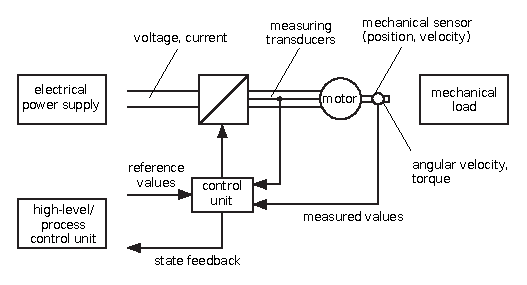
\includegraphics[width=0.8\columnwidth]{sota/electric_drive.eps}
         \caption{Electric drive scheme (See: \cite{Boecker2016})}
         \label{fig:edrive}
\end{figure}

%%Unterschied PMSM von anderen Synchronmaschinen
Among several types of synchronous electric machines \gls{pmsm} devices offer characteristics meeting particularly the demands in industrial and automotive applications.
Their  high efficiency,  high torque/power density and high torque-to-inertia ratio as well as maintenance-free operation make them the optimal choice in most cases.
Like all AC motors the \gls{pmsm} consists of a stator and a rotor.
As it belongs to the group of synchronous motors its rotor cycles synchronously with the frequency of the supply current in the stator.
The distinguishing feature of a \gls{pmsm} contrary to other synchronous machines is the incorporation of permanent magnets embedded in the rotor.
These magnets provide a static magnetic field rotating with the rotor and substitute the supplement by electromagnets.
The advantages are less mass inerta in the rotor due to the lack of windings and less maintenance requirements for the commutator \cite{LeVa2014, Schroeder2007}.

%%Welcher Motor wird verwendet und wie sieht ein Querschnitt aus
The motor considered in this work is a \SI{60}{kW} automotive traction PMSM prototype.
Some of its important components - in particular the stator yoke, stator tooth and permanent magnets - are depicted in fig. \ref{fig:pmsm_cross_section} \cite{WaBo2016}.
\begin{figure}
	\centering
	\def\svgwidth{0.6\columnwidth}
         \import{eps/sota/out/}{pmsm_cross_section.pdf_tex}
         \caption{Cross section of the investigated \gls{pmsm} incorporating interior magnets and concentrated windings (Source: \cite{WaBo2016})}
	\label{fig:pmsm_cross_section}
\end{figure}

%%Gliederung PMSM
Section \ref{ssec:pmsm_basic} introduces the basic modeling and operating constraints \cite{LeVa2014, Schroeder2007} whereas sections \ref{ssec:pmsm_loss_heating} and \ref{ssec:pmsm_thermal_model} give insights to occurring power losses \cite{Kylander1995, Roberts1986, Schroeder2007} and thermal modeling \cite{ BoCa2009, LeVa2014, MeRo1991, WaBo2016}, respectively.

\subsection{Basic Modeling And Operating Constraints}
\label{ssec:pmsm_basic}
%%Spannung und Strom in dq-Koordinaten
Describing the basic behavior of the \gls{pmsm} a coordinate system rotating with the rotor in phase is convenient.
The resulting orthogonal axes are noted $d$ and $q$ where the former is aligned with the rotor's permanent magnetic field.
In steady state, both explain important electric quantities in a time-invariant fashion.
The coordinate system's angular velocity is given by $\omega_{el} = p\omega_{mech}$, where $p$ denotes the pole pair number and $\omega_{mech}$ describes the rotor's mechanical angular velocity.
Neglecting magnetic anisotropy and (cross-)saturation effects the voltage in $dq$-coordinates derives to
\begin{align}
	u_{sd} = R_s i_{sd} + L_s\frac{\dif{i_{sd}}}{\dif t} - \omega_{el} L_s i_{sq} \\
	u_{sq} = R_s i_{sq} + L_s\frac{\dif{i_{sq}}}{\dif t} + \omega_{el} L_si_{sd} + \omega_{el} \Psi_p.
\end{align}
Here, $R_s$ stands for the stator resistance, $i_{sd}$ and $i_{sq}$ for the current on the $d$ and $q$ axis, respectively; $L_s$ denotes the self inductance and $\Psi_p$ represents the permanent magnet flux linkage.
These equations' equivalent circuit diagram is depicted in fig. \ref{fig:eq_pmsm_scheme}.

\begin{figure}
        \centering
        \def\svgwidth{0.7\columnwidth}
        \import{eps/sota/out/}{equivalent_scheme_dq_coordinates.pdf_tex}
        \caption{Equivalent PMSM scheme (See \cite{LeVa2014, Schroeder2007})}
        \label{fig:eq_pmsm_scheme}
\end{figure}
Following this notation, the electromagnetic torque $T$ can be described by
\begin{align}
	T = \frac{3}{2}p\Psi_pi_{sq},
\end{align}
which inherently shows the required $q$-axis current for a desired torque.
As for every physical system, constraints need to be taken into account with one of them being certain limitations for the current and voltage amplitude:
\begin{align}
	|U| = \sqrt{u_d^2 + u_q^2} \leq |U|_{lim}\\
	|I| =  \sqrt{i_d^2 + i_q^2} \leq |I|_{lim}.
\end{align} 
As losses typically scale with the stator current amplitude $|I|$, one would usually opt for minimizing $i_d$ as far as possible, $i_d = 0$ at minimum.
More on losses in the next sections.

Note, that the motor parameters $L_s$, $\Psi_p$ and $R_s$ are not constant over the operation range due to temperature and saturation effects causing the analytical calculations to become unreliable.

\subsection{Power Losses and Heating}
\label{ssec:pmsm_loss_heating}
%%Verlustarten (Welche Verluste treten in PMSM grob auf, weshalb und wo)
Losses in synchronous machines  are divided into two categories based on their source and dependency: Load losses and no-load losses.
As one can infer from their nomenclature, no-load losses are load-independent while load losses strongly depend on the load and the currents.

\subsubsection{No-Load Losses}
%% No-load loss
In particular, the following losses are to be expected at no load:
\begin{itemize}
	\item Iron core losses in the stator teeth and yoke, evoked by the main flux through reversal of magnetism,
	\item losses due to friction and windage and
	\item no-load stray losses and other minor losses.
\end{itemize}
Core losses describe eddy current losses and hysteresis losses, which are proportional to the frequency and the peak flux density.
Calculating these losses is difficult as manufacturing variations, harmonics and temperature affect them significantly.

Losses due to friction typically occur in the bearings and their sealings.
The ratio between the losses in the bearings and those in the bearing sealings are generally not known \textit{a priori}.
Windage losses occur by the incorporation of a cooling fan but as they come with the fan's cooling ability they don't cause an increase in heating.

The last item summarizes those losses of no fundamental frequency e.g. flux harmonics inside the magnets, surface losses or resistive losses due to the no-load current. 

\subsubsection{Load Losses}
%% Load losses
Load losses, on the other hand, consist of resistive losses in the stator winding and losses evoked by the leakage flux and space harmonics.
For a non-sinusoidal supply voltage there are considerable harmonic losses increasing the resistive losses in the stator windings due to harmonic currents and the skin effect.
Furthermore, core and surface losses grow because of the harmonic flux components.

\subsubsection{Heat Transfer}
%% Unterschied conductive and convective
Heat flow is either conductive, convective or based on radiation.
The latter is negligible relative to the former two forms of heat transfer in case of synchronous motors.
Conductive heat transfer happens within solid components and is modeled in a cylindrical rod structure in most cases.
Convection, further, describes transfer processes based on fluid motion (air or liquid).
That could be heat transfer from solid components to the internal air within the enclosed motor and from there, again, to ambient air.
Having a build-in cooling fan or a liquid cooling system, forced convection would boost motor cooling.
Otherwise, convective heat transfer is by free convection only.  

\subsection{Thermal Modeling}
\label{ssec:pmsm_thermal_model}
Naturally, the motor's current-dependent losses and, thus, its heating are primarily influenced by the motor's operation mode.
Typical operation modes are defined in VDE standard 0530 \cite{VDE0530}, which play an important role in the construction of every motor.
However, the thermal environment in automotive applications is challenging and requirements on power density and reliability as well as pricing pressure urge motors to their limits.
High temperatures due to overload will damage the stator windings' insulation varnish and reduce the device lifetime considerably.
Besides that, perseverative high thermal stress degrades the permanent magnets' material and can ultimately lead to their irreversible demagnetization.
Hence, precise thermal analysis became an indispensable tool and thermal management technology experiences growing attention.

The motor is a thermal system consisting of different components in certain constellations (stator, rotor, windings, air gap etc.), where each has its own thermal characteristics.
Analyzing the thermal behavior of this system as a whole is non-trivial.
Nowadays there are two basic approaches to the thermal modeling of electric motors: analytical lumped-circuit (with the optional aid of empirical data) and numerical methods.
Their main differences lay in the required computational time, achieved precision and geometrical limitations.

Regardless of which technique is practiced a designer of thermal models often has to determine thermal resistances beforehand.
Calculating these thermal resistances goes by simple, well established equations for every kind of heat transfer (conduction, convection and radiation).
However, the equations' parameters are partly difficult to define as they depend not only on geometry but also on e.g. fluid turbulence or the interface gap between components.
As a consequence, modeling quality benefits from a designer's experience and the accuracy of material parameter data sheets.

For the numerical approach there are two well established types \cite{BoCa2009}: \gls{cfd} and \gls{fea}.
Regarding the analytical approaches \cite{BoCa2009, MeRo1991, WaBo2016}, the methodology of \glspl{lptn} are described below and their particular shortcomings are worked out in order to motivate this work's purpose.

\subsubsection{Numerical Analysis}
Numerical analyses emerged in the 1990s with the advancements in computational capacities.  
While being capable of modeling any device geometry is a highly appreciated advantage of numerical approaches, the high demand in computational time and model setup prevent them from being of practical use outside the construction phase.
Nevertheless, due to their relatively precise modeling capabilities they play important roles in research and development.

%%FEA
The main purpose of \gls{fea} is the accurate determination of conductive heat transfer within and between solid components of almost arbitrary geometry.
Its time-consuming factors consist of mesh definitions for the model setup and heat-field computations.
Though its application takes a considerable amount of time, it is able to find non-linear loss distributions across the electric machine and a non-symmetrical operational flux density. 
\gls{fea} can also be used as previous step to network analysis for accurate thermal conductivity calculation and to define more accurate loss injections in the network nodes as well as for the determination of the thermal-network discretization level.
There is a thermal and an electromagnetic variant of \gls{fea}, each for its corresponding purpose of analysis, but this does not preclude a combination of both, which can lead to temperature-dependent loss computations.
Unfortunately, similar to \glspl{lptn}, \gls{fea} suffers from imprecise thermal resistance computations and material parameter data.
Moreover, while conductive heat transfer computations are usually excellent, good results are more difficult to achieve for the convective counterpart.

%%CFD
The application of \gls{cfd} principally aims for the computation of the rate and velocity of the coolant flow.
Further it gives evidence about surface heat transfer and pressure distributions in the cooling passages within the machine.
Conversely, \gls{cfd} provides reasonable support for fan design as fans incorporated in electric machines often constitute poor efficiency in an aerodynamic matter due to competitive pressure.
When designing thermal models via \gls{cfd}, building an accurate mesh without excessive cell numbers represents the biggest challenge.
Though it is beyond the scope of \gls{cfd}, there are attempts to model conduction with it, too, yet \gls{fea} is undoubtedly the better choice.
However, the insights gained by \gls{cfd} can help to improve the analytical algorithms in a \gls{fea} model or in thermal networks.

\subsubsection{Thermal Management}
%%Passive thermal management is bad
Although through specification of certain limits to the maximum torque or current rating - including relatively large safety margins - thermal induced damage indeed can be avoided, this will cause an inevitable constraint on the performance.
While rating limits are specified in motor/inverter data sheets they don't take any current temperatures into account and are, thus, mere passive means to thermal management.
Since these limitations have to consider worst-case scenarios, there are several circumstances where large performance potential remains unused. 
When operating at, for example, low ambient temperatures, the heat dissipation capabilities of the components are naturally higher than rated.
In addition, at high operation frequency, junction temperature fluctuations are typically smaller, whereas limiting ratings are defined for the more demanding operation at low frequencies.
Moreover, since fixed current limits account for steady-state operation, the materials' short-time thermal overload capacities can't be utilized. 

%%We need online temperature information
As a consequence, further sophisticated methods should be conducted in order to improve lifetime as well as gaining the maximum performance off the material and utilizing thermal overload capacities without risk of reliability loss.
Here comes online temperature monitoring into play:
online temperature information allows not only safe motor operation but also maximum device utilization in terms of power/torque density.
The naive approach depicts sensor based measurements.
In fact, as pricing pressure is high in the automotive environment and sensors incorporated in particularly rotating parts of an electric machine is tied up with frequent maintenance and error-proneness, this approach is usually not feasible.
Therefore, parametric models with low-computation and less time-consuming properties are the primary choice.
Thermal networks meet those requirements.

\subsubsection{Thermal Networks}
%Thermische Netzwerke (oberflächlich, typische Struktur und Analogien zu el. Ersatzschaltbildern aufzeigen.
Thermal networks show a specific advantage over numerical approaches:
High calculation speeds for low-order networks make the \gls{lptn} suitable for online temperature monitoring.
\glspl{lptn} offer two types of calculation: heat-transfer and flow-network analyses.
The former stands for the thermal counterpart and the latter for the fluid dynamics counterpart to electrical-network analysis.
The equivalences are given in tab. \ref{tab:heat-transfer}.
\begin{table}
		\caption{Equivalences between heat-transfer thermal networks, flow networks and electrical-network circuits}
		\label{tab:heat-transfer}
		\centering
		\begin{tabular}{l l l}
			\toprule
			thermal networks & flow networks & electrical-network circuits \\
			\midrule
			temperature & pressure & voltage\\
			power & volume flow rate & current\\
			thermal resistance & flow resistance & electrical resistance \\
			\bottomrule
		\end{tabular}
\end{table}

In the heat-transfer network thermal resistances would represent main power flow paths between components, which give rise to temperature predictions.
Moreover, thermal networks help defining the necessary discretization level of electric motors.
While in the past relatively simple thermal networks with few nodes were designed, more detailed circuits with more thermal and flow elements can be computed in a fair amount of time today.
A low-order \gls{lptn} is exemplified in fig. \ref{fig:lptn} \cite{WaBo2016}.
\begin{figure}
	\centering
	\def\svgwidth{0.8\columnwidth}
         \import{eps/sota/out/}{lptn.pdf_tex}
         \caption{Example structure of a low-order \gls{lptn} (Source: \cite{WaBo2016})}
	\label{fig:lptn}
\end{figure}

%%Herauskitzeln warum therm. Networks schwierig zu erstellen sind um den Einsatz von NNs besser zu motivieren).
Due to the fact that several thermal phenomena inside electric machines are not analytically solvable in a closed relationship, designing thermal models with sufficient accuracy proves a difficult task even when geometry and material data is known exactly. 
In order to improve prediction performance to an acceptable level, it is common to take empirical data into account to adjust the \gls{lptn} parameters.

Another concern that necessitates experimental measurements is the fact that, in a real-time context, \glspl{lptn} are only feasible in a limited order of complexity.
In other words, the more nodes and elements considered in a \gls{lptn}, the higher the amount of differential equations are subject to computation, which is bounded by the computational capacities of the electronic control unit.
Especially in automotive applications, where the electronic control unit depicts a bottleneck due to its multi-task demands, just relatively small thermal networks prove practical.
Since lower orders of abstraction mean less spatial precision in temperature estimation, those networks rely on additional empirical data in order to not miss hot-spot temperature information.

%%Problem of varying model parameters (e.g. Konvektionswiderstände) bzw. varying model input quantities (e.g. Motor losses and their influencing quantities)
A further problem thermal network designers have to face are varying model parameters e.g. thermal resistances between stator and rotor change due to the motor speed influencing the air gap convection.
Overcoming this problem of linear parameter-varying systems one either has to follow a local approach, where multiple independent experiments are conducted in order to receive a local LTI model for each experiment, or, conversely, one follows a global approach, in which model parameters are directly found through one comprehensive experiment.
For the former, merging all local LTI models together leads to non-robust and possibly inconsistent models, which inherently lack the overload operation range and make the identified \gls{lptn} valid for only a subset of applications.
Going for the global approach, one receives more robust results but this comes with the prerequisite of considering more \textit{a priori} knowledge and predefinition of certain parameter relationships by the model designer.

As developing thermal networks is a demanding task where model designers often have to trade off complexity order (respectively estimation accuracy) against real-time feasibility and where model structures based on heat transfer theory are skewed by the incorporation of experimental data for the benefit of prediction quality, this work investigates the black-box approach of \glspl{ann} as thermal models for electrical traction drives, in particular for the \gls{pmsm}.

%Anwendungskontext (Automobilbereich: Sehr viele exogene Einflussgrößen zB Lastprofil aufgrund Fahrerverhalten, Fahrstrecke bzw. Verkehrslage oder ext. Temperaturen etc). 
%Diese stochastischen Einflüsse erschweren daher das Schätzproblem  und ergeben die Schwierigkeit der Aufgabenstellung.
%Short periods of high demand. Low average power output.

\section{Machine Learning And Artificial Neural Networks}
\label{sec:ml_ann}
%Wo waren sie bereits erfolgreich?
Utilizing \glspl{ann} has proven feasible in many fields of research and often offer state-of-the-art performance.
Especially in the field of automatic speech recognition - both large scale acoustic modeling and language modeling - breakthroughs through the utility of neural networks have called much attention and leveraged their application \cite{GraSchmi2005, SaSe2015, SakHa2014}.
Moreover, there are certain neural network applications in the field of computer vision claiming state of the art in object recognition \cite{LiHu2015}, image generation \cite{GreDa2015} and captioning images/videos \cite{DoHe2014, MaXu2014}.
Furthermore, they have been successfully used in handwriting recognition \cite{DoKo2014, GraLi2009} and in audio analysis \cite{MaFe2014}.
There were even significant advancements in machine translation \cite{LuSu2014} and in predicting protein secondary structure \cite{SoWi2014}. 

A comprehensive and contemporary review of neural networks is given by \cite{Lipton2015}.
The reason for the neural networks' success is attributed to their learning abilities going beyond mere hand-engineered features to learning hierarchical representations and exploiting raw non-determinable features.
The more training and test examples are available for the supervised learning of \glspl{ann} the more does the model benefit from it, as opposed to other models for cognitive and perceptive tasks.
Linear models, for example, tend to under-fit data with a vast amount of data instances and fail to utilize the ever-growing computing capabilities and memory storages nowadays.

%HMMs 
In terms of sequence modeling, \glspl{hmm} represent a considerable competitor to \glspl{ann}.
\glspl{hmm} predict observable sequences given a sequence of unobservable states in a probabilistic fashion.
This is useful in, for example, acoustic modeling, where spoken words are recognized regardless of the speed of speech due to the discreteness of the state space.  
However, HMMs loose their souvereignty quick as soon as the number of hidden states grows large in order to achieve higher expressive power.
Since computing time and the table of transition probabilities rise quadratically with the number of hidden states, computation gets infeasible as of medium-sized state spaces already.
In addition, for the state space being discrete, the expressive capability is even further capped naturally.
Besides that, an important drawback of the \gls{hmm} postulation is the dependency of each hidden state on its previous state only.
This prevents the model to consider long-range dependencies in long sequences, which is essential in plenty of cognitive tasks such as speech recognition, machine translation or any other field where time series have to be predicted.
There have been proposals to extend the accounted context window but they come with a large extra amount of computation condemning the already computation-heavy \glspl{hmm} to perform poorly next to its competitors.

% RNNS too expressive? every NN is differentiable end to end. Gradient based training! There is regularization to prevent overfitting
One important attribute of \glspl{ann}, which differs them from arbitrary models with a similar expressive power, such as a program in C, is the fact that, given the structure and set of its free parameters, they are differentiable end-to-end.
While a written piece of code can theoretically solve any computable task, its search space cannot be explored efficiently.
However, neural networks provide a general way to determine the gradient to the minimization of a chosen loss function with respect to the neural networks' weights, that are its adjustable parameters.
This makes the well studied methodology of gradient-based training applicable.
Furthermore, while present for a lot of models with high expressive capabilities, the problem of over-fitting data during machine learning, that is learning the seen data ``by heart'' without being able to generalize to new data, can be mitigated for the case of \glspl{ann} by several proposed regularization techniques.   

%Wie viel Speicher brauchen NNs auf dem Feld? Wie computational heavy ist deren Einsatz?
Real-time applications benefit from the lightweight utilization of \glspl{ann}.
While training neural networks is computational heavy and time consuming, even more for vast amounts of training examples and bigger nets with a lot of parameters, once training has finished, calculating an output from a given input is significantly faster.

There are diverse architectures leading to varying results in different fields of application and one has to consider each architectures advantages and drawbacks.
The basic \gls{ann}, first proposed in the 1950s, also known as \gls{mlp} or \gls{fnn}, provides undoubtedly the least potential, though it lends itself well for an introduction to the matter.
Aside from the application in the field of computer vision, the \gls{rnn} architecture is the most deployed net among time series modeling tasks together with its variants, for instance, the \gls{lstm}.
Since the \gls{lstm} is frequently applied in this work, it will be explained particularly in the next chapter.
%
%Gliederung
%First of all, in subsection \ref{ssec:basic_topologies} the very basics of \glspl{ann} are introduced and illustrated using the example of a \gls{fnn} and a \gls{rnn}.
%Although not applicable for this work, but nonetheless worth mentionable architectures are outlined as well in subsection \ref{ssec:other_archs}.
%After that, we dive into training neural networks in subsection \ref{ssec:training}, where a brief mathematical derivation is covered.

\subsection{Basic Topologies Of Artificial Neural Networks}
\label{ssec:basic_topologies}
The inspiration for establishing \glspl{ann} was taken from the biological functionality of the human brain.
Each neural network consists of an \textit{input} and \textit{output layer}, one or more \textit{hidden layers}, and a set of \textit{artificial neurons}, also referred to as \textit{units} or \textit{nodes}.
The counterpart to biological synapses are represented by directed edges between the neurons.
Though in the early years of the \gls{ann} history efforts were made to keep the biological analogy, it was soon neglected for the benefit of empirical results.
Each neuron takes arbitrary many input edges and produces exactly one output, which can again be forwarded to arbitrary many other neurons as input.
Moreover, each neuron has a differentiable activation function associated with, which will ensure end-to-end differentiability.
The non-linear function, the neural network is describing eventually, is determined by its set of variable parameters, that are real-valued weights allotted to each directed edge.
It is common practice to allow for an offset weight for each neuron, which further enriches the neuron's expressive power.

Since notation differs throughout the broad range of papers regarding \glspl{ann}, this work sticks to the notation introduced in \cite{Lipton2015} as special emphasis was placed on clean formalities there.
We call a weight associated with an edge from node $j'$ to $j$ as $w_{jj'}$, following a ``to-from'' index notation.
The real-valued output $v_j$ of a node $j$ is the result of its activation function $l_j(\cdot)$ applied to the weighted sum of the node's incoming input edges plus its offset $b_j$:
\begin{align}
	\label{eq:fnn_single_weight}
	v_j = l_j \left( b_j + \sum\nolimits_{j'} w_{jj'} \cdot v_{j'}\right).
\end{align}
Vector notation allows a comfortable description of a whole layer's calculation:
\begin{align}
	\label{eq:fnn}
	\bm{h} = l_h \left( \bm{W}^{hh'} \cdot \bm{h}' + \bm{b}_h \right).
\end{align}
Here, $\bm{h}$ denotes the vector of the current layer's nodes' output values, $\bm{h}'$ those values from the previous layer,  $\bm{W}^{hh'}$ stands for the weight matrix from the previous layer $h'$ to the current layer $h$ and $\bm{b}_h$ notates the current layer's bias vector.
The function $l_h$ represents the activation function for every neuron in the current layer.
Though this is seldom the case, the activation function per neuron can theoretically vary within a layer.
Yet, since this does not apply to most scientific proposals and has no proven benefit, it is assumed here, that each neuron in a certain layer has the same activation function.
The input's and output's data dimension determines the number of neurons in the input and output layer, respectively.

Common activation function candidates are the \textit{tanh} function $\phi(z)=(e^z - e^{-z})/(e^z+e^{-z})$, the \textit{sigmoid} $\sigma(z) = 1/(1 + e^{-z})$ and the \textit{\gls{relu}} $l(z) = max(0, z)$, where the latter was introduced in machine learning research recently with significantly improved results (see \cite{BeBou2013}, for example) giving rise to some other parametric variants.
The activation function of the output layer's nodes is dependent upon the model's purpose.
Having a classification task to solve with $K$ distinct classes, a softmax nonlinearity is applied to $K$ nodes in the output layer, where the output values of all nodes sum to one through the softmax function's normalizing term.
In order to model regression tasks the output nodes' activation function simplifies to the identity function.

Regarding the number of hidden layers: It is mathematically proven, that a standard neural network with just one hidden layer ``is capable of approximating any measurable function to any desired degree of accuracy, in a very specific and satisfying sense.'' \cite{HoSti1989}.
However, it has been shown, that shallow networks often perform insufficiently and plenty of tasks with non-determinable abstract features - especially where the input-output-relation is diffuse - require \textit{deep architectures} with several hidden layers in order to achieve state-of-the-art results \cite{Bengio2009}. Training a deep model is often referred to as \textit{deep learning} and exhibits new challenges in comparison to shallow models.

Within the scope of this work, input and output data always describe temporal sequences.
Hence, further subsections will always point out the impact of specific structures and methods on time series based applications.
Nonetheless, all following observations are also applicable on data without temporal context.

The maximum time index of an investigated data sequence is specified by $T$, yet the case $T \to \infty$ is theoretically not excluded.
Input and target sequences are denoted $\left(\bm{x}^{(1)}, \bm{x}^{(2)}, \ldots, \bm{x}^{(T)}\right)$ and $\left(\bm{y}^{(1)}, \bm{y}^{(2)}, \ldots, \bm{y}^{(T)}\right)$, respectively.
In contrast, a model's predicted output is labeled as $\bm{\hat{y}}^{(t)}$.
Note the superscript in parenthesis to emphasize temporal position as against superscripts without parenthesis for node and layer indices.
Having this terminology set up, an investigated sequence comprises multi-dimensional data points $\bm{x}^{(t)}$ seen by the model one by one in a discrete fashion, where each distinct time step is indexed by $t$.
Each input and target sequence form an example pair and all pairs a full set.
During training the whole considered data is usually called the training (sub-)set. 

\subsubsection{Feedforward Neural Network}
\glspl{fnn}, or \glspl{mlp} synonymously, represent the simplest architecture for neural networks.
They restrict propagation of calculations to one way, from input to output, precluding cycles from higher layers to previous layers or within a hidden layer.
Fig. \ref{fig:fnn} depicts the structure of a simple \gls{fnn} with one hidden layer of three hidden neurons and two neurons for each the input and output layer.
Beginning from the input data $\bm{x}$ each subsequent layer computes its neurons' output values $\bm{h}$, propagates them to the next layer and, ultimately, the output layer returns the result $\bm{\hat{y}}$.
\begin{figure}
	\centering
	\def\svgwidth{0.6\columnwidth}
         \import{eps/sota/out/}{fnn.pdf_tex}
         \caption{\gls{mlp} with one hidden layer}
	\label{fig:fnn}
\end{figure}

The major drawback of \glspl{fnn} is the fact, that they inherently assume consecutive shown data to be independent from each other.
This prevents them from learning any temporal context during learning of sequences or time series.
Yet many important real-world tasks hold temporal dependencies.

\subsubsection{Recurrent Neural Network}
In an attempt to tackle the problem of missing temporal context utilization \glspl{rnn} were introduced.
Their basis is a \gls{fnn} but augmented with timely delayed cycles back to the input of the same layer the cycles have their origin at.
These cycles are called \textit{recurrent} edges and they also include paths from a neurons output to the same neurons input, though they are only attached to hidden layers.
The augmented topology is illustrated in fig. \ref{fig:rnn}, where the neural net holds the same amount of neurons and hidden layers as in the previously exemplified \gls{fnn} structure.
\begin{figure}
	\centering
	\def\svgwidth{0.6\columnwidth}
         \import{eps/sota/out/}{rnn.pdf_tex}
         \caption{\gls{rnn} with one hidden layer (output specifiers omitted to ease clutter). Recurrent edges channel their values at time $t$ back to the layer's input at time $t+1$. }
	\label{fig:rnn}
\end{figure}

Having recurrence incorporated, temporal dependencies find their way to the model.
Analytical calculation is presented for a \gls{rnn} with one hidden layer to keep the matter simple.
At each time step $t$, hidden layer nodes generate an output $\bm{h}^{(t)}$ by receiving current data $\bm{x}^{(t)}$  from the previous layer (here: the input layer) and simultaneously from the same layer's output $\bm{h}^{(t-1)}$ at the earlier time step $t -1$.
The neural network's output $\bm{\hat{y}^{(t)}}$ is thus influenced by the hidden and input layers' nodes' states at previous time steps.
Note, that this topology considers past temporal context only.
Calculating the sole hidden layer's output, equation \ref{eq:fnn} changes to:
\begin{align}
	\bm{h}^{(t)} = l_h\left(\bm{W}^{hx}\bm{x}^{(t)}+\bm{W}^{hh}\bm{h}^{(t-1)}+\bm{b}_h\right),
\end{align}
and for the predicted output $\bm{\hat{y}}^{(t)}$ at time $t$ follows:
\begin{align}
	\bm{\hat{y}}^{(t)} = l_y\left(\bm{W}^{yh}\bm{h}^{(t)}+\bm{b}_y\right).
\end{align}
These equations show temporal indices for the current time step $t$ and the earlier time step $t-1$.
Matrix $\bm{W}^{hx}$ comprises weights associated with the edges from the input layer $x$ to hidden layer $h$, whereas $\bm{W}^{hh}$ and $\bm{W}^{yh}$ explain weights of the recurrent edges and from the hidden layer to the output layer $y$, respectively.
The bias vectors $\bm{b}_h$ and $\bm{b}_y$ represent offset for the respective layers.

In order to support comprehension of the temporal dynamics of a \gls{rnn}, it is possible to unfold the cyclic visualization across time steps.
Fig. \ref{fig:unfold} shows the same simple \gls{rnn} as in fig. \ref{fig:rnn} but with the mentioned principle applied.
This network can be interpreted as deep network with one hidden layer per time step and each layer sharing the same weights.
In this illustration it is highlighted how input data from earlier time steps manages to remain in the network and influences the neural networks' output at a later time step.
\begin{figure}
	\centering
	\def\svgwidth{0.8\columnwidth}
         \import{eps/sota/out/}{unfold.pdf_tex}
         \caption{A \gls{rnn} unfolded across time steps. The highlighted route represents information entering the networks hidden layer, partly remaining there and affecting the networks output at every next time step.}
	\label{fig:unfold}
\end{figure}

\subsection{Other Architectures}
\label{ssec:other_archs}
This subsection shall give an overview of those architectures, which are not investigated in this work.
Emphasis is placed on the motivation and deficiencies of each approach.
The following topologies were not contemplated because either they were not applicable to this thesis' underlying task or would go beyond the scope of this work.
Some of them are simply inferior to other more advanced approaches.

\textit{\glspl{tdnn}} are networks of the feed-forward type, trying to utilize past temporal context \cite{LaWa1990}.
The input sequence is cascaded into successively delayed lines, which act as distinctive features.
Propagating the delayed sequences through the net at once, the topmost layer would receive the whole time window.
Initially introduced to represent a superior approach to \glspl{hmm} in speech recognition, \glspl{tdnn} soon were outshined by its competitor's advancement.

There are certain proposals, where \textit{\glspl{narx}} are combined with \glspl{rnn} \cite{LiBi1996}.
It has been shown, that this particular model may mitigate the vanishing gradient problem of \glspl{rnn} and is capable of learning long-term dependencies two to three times further in the past than mere \glspl{rnn}.
Anyhow, it does not circumvent this fundamental drawback.
Both, \gls{tdnn} and \gls{narx}-\gls{rnn} appear in nowadays scientific papers time and time again, despite their well-known insufficiencies.
One possible reason might be, that these architectures are supported by MATLAB's neural networks toolbox offering an intuitive handling, especially for researchers new to the matter.

An important milestone in neural network research was set with the introduction of bidirectionality to \glspl{rnn}, namely the \textit{\gls{brnn}} and \textit{\gls{blstm}}, which has let to an breakthrough in phoneme classification and handwriting recognition \cite{GraSchmi2005, SchuPa1997}.
Its strength is embodied by the ability to learn context dependencies not just from past data but also from data yet to come during each time step.
Trivially, this comes in handy for applications without real-time demands only, since fixed length sequences are required in the first place.

\textit{Clockwork} \glspl{rnn} \cite{KoGre2014} are a recent alternative augmented by clock rates.
It consists of an \gls{rnn} with one hidden layer, which is partitioned into separate modules, each calculating input data at a different and predefined clock rate.
The purpose of processing sequences at different temporal granularities separately is to address the different dynamic time-scales within time series.

Another novel approach is the \textit{gated feedback} \glspl{rnn} \cite{ChuCa2015}.
It extends the standard topology of deep \glspl{rnn} by global gates between hidden layer pairs, that is, channels from upper layers to the immediately lower layer with adaptive weights.
This further encourages modeling of both, fast changing and slow changing components in the input sequences.
The initiators, \textit{Chung et al.}, want their approach to be understood as a generalization to the clockwork \gls{rnn}, as they embed hierarchically stacked modules across hidden layers, in which the feedback gates adaptively find a proper processing rate.

In the application field of computer vision, \textit{multi-dimensional} \glspl{rnn} were proposed \cite{GraFe2007} performing decent, though they were trumped by \textit{\glspl{cnn}} holding the state of the art until present time \cite{KriSu2012}.
The topology of a \gls{cnn} is of the multi-layered feed-forward category exploiting spatially-local correlation within the input images.
Here, subgroups of neurons are limited to an enclosed, specific receptive field and learn to represent filters or kernels by reacting on certain features at specific spatial positions in the input images. 
One of their strong characteristics is, that they require very little pre-processing of the input images, making their application relatively effortless.

Architectures incorporating an addressable external memory resource are described by e.g. \textit{memory networks} \cite{WesCho2014} and \textit{\glspl{ntm}} \cite{GraWa2014}.
The difference of the former with respect to the latter is a larger memory storage, less complexity and its focus on language and reasoning tasks.
The \gls{ntm} improves upon the capabilities of \glspl{rnn} to solve algorithmic tasks e.g. sorting or copying.
Algorithmic tasks are those, that a simple program could calculate with the very detail of \glspl{ntm} being end-to-end differentiable.
A further advancement is proposed by \textit{pointer networks} \cite{ViFo2015}.
They facilitate attention-mechanics (not outlined in this work, see for example \cite{ChoBa2015, XuBa2015}) as pointer to input elements substituting members of the output sequence.
By doing this, pointer networks are shown to solve sorting tasks with variable sized sequences and certain combinatorial optimization problems.

\subsection{Training Neural Networks}
\label{ssec:training}
The machine learning community separates training into three categories \cite{Bishop2006}:
\begin{itemize}
	\item Unsupervised learning,
	\item Supervised learning and
	\item Reinforcement learning.
\end{itemize}
The first option describes the training of models by giving input training data without corresponding target data.
The expected result is finding coherent subgroups within the data, so called \textit{clusters}, where data members of the same group share more similar attributes rather than those in different clusters.
Other purposes are to estimate the data's probability distribution or to reduce the data's dimension to fewer, more explaining dimensions.
A neural network learning efficient codings during unsupervised learning is called an \textit{autoencoder}.

In contrast, supervised learning represents model learning by ``showing'' corresponding input and optimal target data subsequently, while the model has to find a suitable mapping for it.
If the target data comprises a finite and discrete set of classes, the task is called \textit{classification}.
Conversely, if the target data consists of continuous variables, it is called regression.
Most of the real world applications are of the supervised learning type, which, in addition, is the most investigated machine learning technique for neural networks in terms of published work.

The other category, reinforcement learning, is concerned with finding the best decision given a situation offering several choices against the background of maximizing a reward or, respective, minimizing a penalty.
An example for reinforcement learning is the task of teaching a machine how to play a chess game, where victory corresponds to a reward.

Since this work's underlying task is of the supervised learning type, the other approaches are neglected during the remainder of this thesis.
As mentioned earlier, during learning, the model seeks to minimize the difference between the target $\bm{y}$ and the prediction $\bm{\hat{y}}$, which is dependent on the input data $\bm{x}$ and the current internal parameters (weights).
The distance between target and prediction is measured by a loss or cost function determined by the model designer in beforehand.
Through iterative adjustment of the weights, that is the process of training or learning, the model tries to minimize the penalizing cost.

During a classification task, the cross entropy is the prevailing choice for the cost function.
Nevertheless, there are other losses that prove more constructive in certain applications, e.g. the \textit{connectionist temporal classification} loss for sequence labeling in the field of automatic speech recognition, where alignments between targets and inputs are unknown. 
Solving a regression task, the broad majority of investigations utilizes the \gls{mse}.
Indeed, all common loss functions that are considered in linear regression modeling can also be of use in a neural network application.
The \textit{root mean square error} or the \textit{Huber} loss are alternatives one might think of, which are less sensitive to outliers than the \gls{mse}.

\subsubsection{Error Backpropagation}
There are multiple approaches to exploring the error surface evoked by the difference between target and prediction.
The prevailing method for \glspl{ann} is \textit{error backpropagation} and, particularly for \glspl{rnn}, \gls{bptt}  \cite{ LeBo1998, Lipton2015, Werbos1990}.
By applying the simple chain rule, backpropagation identifies the derivative of the loss function with respect to every weight in the neural network.
Thereupon the weights are tuned accordingly.
Error backpropagation encompasses various optimization techniques confining themselves to calculating the loss' first-order derivative only.
The simplest and moderately common variant is \gls{sgd} in conjunction with combining multiple training examples to mini-batches.
\gls{sgd} is called stochastic, since it does not consider all data for each update step but just one single observation.
The incorporation of mini-batches mitigates the stochasticity.
More on the purpose of mini-batches is addressed in section \ref{sec:opt}.
Neglecting them for now, the \gls{sgd} update equation with the cost function $\mathcal{L}_i$ is described by
\begin{align}\label{eq:sgd}
	\bm{w}\gets\bm{w}-\eta\nabla_{\bm{w}}\mathcal{L}_i 
\end{align}
with $\eta$ being the step size or learning rate and $\nabla_{\bm{w}}\mathcal{L}_i $ the objective's gradient with respect to the weights $\bm{w}$ after having seen the single data pair $(x_i, y_i)$.
The learning rate factor is a crucial parameter, which needs to be defined by the model designer in the first place.
Having a too large learning rate, training would diverge quickly, while a too small rate leads to unnecessarily slow training.

In order to mitigate clutter, the term \textit{net activation} is introduced, representing the sum inside the parenthesis in equation \ref{eq:fnn_single_weight}, that is $a_j =  b_j + \sum\nolimits_{j'} w_{jj'} \cdot v_{j'}$, and shall support following equations.
Before gradients can be calculated, a complete forward pass needs to be conducted, such that we have a value $v_j$ at each neuron and the predictions $\bm{\hat{y}}$ at the output layer.
Then, the distance between target $y_k$ and prediction $\hat{y}_k$ for each output neuron $k$ is determined by the chosen loss function $\mathcal{L}(\hat{y}_k, y_k)$.
Subsequently, by applying the chain rule, the sensitivity $\delta_k$ for output neuron $k$ is defined by
\begin{align}
	\delta_k = \frac{\partial\mathcal{L}(\hat{y}_k, y_k)}{\partial\hat{y}_k}\cdot l'_k(a_k).
\end{align}
Remember, that the activation function $l_k$  for the output neuron $k$ is chosen as identity function, in case of regression tasks.
Beginning with the output neurons' sensitivity, we calculate the sensitivity of each neuron $j$ in the immediately preceding layer by
\begin{align}
	\frac{\partial\mathcal{L}}{\partial a_j} = \delta_j = l_j'(a_j)\sum\nolimits_k\delta_k\cdot w_{kj}.
\end{align}
Applying this calculation for each successive layer yields every node's sensitivity by accounting for the sensitivities of all nodes connected by an outgoing edge from the considered node.
Having produced all values $v_j$ during the forward propagation and all sensitivities $\delta_j$ during the backward propagation, we obtain the cost's derivative with respect to a certain weight $w_{jj'}$ with
\begin{align}
	\frac{\partial\mathcal{L}}{\partial w_{jj'}} = \delta_jv_{j'}.
\end{align}
It becomes evident, that weights with a larger negative impact on the loss function in terms of minimization will experience more fundamental updates than those with less pathological influence.

The principal downside of \gls{sgd} and all its variants is the fact, that it is sensitive to local minima and, thus, the global minimum might never be found.
Furthermore, saddle points cease converging speed as long as step size is set constant.

% vanishing gradient problem
In case of \glspl{rnn}, the optimization is considered as \gls{bptt} because the obtained derivatives also account for the specific time step.
Since the inherent recurrence is also interpretable as infinitely deep topology with shared weights across time steps, a profound problem occurs for the gradient determination.
As the recurrent edge's weight remains the same quantity for every time step, this neuron's input contribution accumulates across time steps.
While the gap between the current time $t$, at which error is calculated, and the earlier time $\tau$, in which the neuron's input provides a contribution to the current time's error, grows large, the corresponding gradients explode or vanish, depending on the recurrent weight being greater or less than one, respectively.
These processes are called \textit{exploding gradient problem} and \textit{vanishing gradient problem}, accordingly.
This prohibits learning long-range temporal dependencies in the training data.
\textit{Pascanu et. al.} deal with this circumstance thoroughly in \cite{PaMi2012}.
A curative solution is given by the incorporation of memory blocks, known as \gls{lstm} (see section \ref{sec:arch}). 

\subsubsection{Methods Incorporating The Cost's Second-Order Derivative}
A presumed advancement to error backpropagation  is the \gls{lm} algorithm \cite{YuWi2011}.
It switches back and forth between error backpropagation and an approximation of the Gauss-Newton algorithm upon the current curvature of the cost surface, which is evaluated through approximated second-order derivatives of the cost function.
When approximating the error function in a quadratic manner is reasonable, the advantageous attributes of the Gauss-Newton method are utilized, which is able to converge directly after the first iteration if a perfect quadratic surface is present.
The \gls{lm} algorithm is more stable than the mere Gauss-Newton algorithm, while converging faster than error backpropagation through the speed up in quadratic environments.
This makes the algorithm very efficient but it also has its drawbacks.
Hessian matrix inversions need to be calculated one or more times per iteration, which is computational heavier and more time consuming the larger the neural network, eventually consuming the whole speed up gained by utilizing the Gauss-Newton algorithm.
Moreover, the Jacobian matrix, which is used for the Hessian matrix approximation, has a size depending not only on the amount of parameters and output units of the neural network but also on the number of features.
This leads the Jacobian matrix storage requirements to let memory cost explode quickly and to counteract the benefit of having more training data.
To make matters worse, the \gls{lm} algorithm is developed for \glspl{mlp} only.
Applying it to \glspl{rnn} is still matter of research.
Nonetheless, the \gls{lm} algorithm is an efficient alternative, as long as the investigated neural network is of limited size and of the feed-forward type.

Another competitor to error backpropagation is \textit{Hessian-free optimization} \cite{Martens2010, SuMa2013}.
Although it leads to competitive results even for deep architectures, it still is an approximation to Newton's method and thus suffers from similar problems as the \gls{lm} algorithm.


    \chapter{Modeling} 
\label{cha:derivation}
%In diesem Kapitel kann das Modell vorgestellt werden, was erarbeitet oder bearbeitet wurde.
%%Purpose, Choice of NNs, Risk
This work's purpose is to investigate the statistical model of \glspl{ann} for its applicability to predicting important component temperatures inside \glspl{pmsm} in a field environment.
The distinctive feature with respect to other models established in this industrial field of research is training the model on empirical data exclusively without incorporating prior analytical knowledge from heat transfer theory.
As neural networks have been successfully applied to other sequence-to-sequence learning tasks (see sec. \ref{sec:ml_ann}) for both, regression and classification, chances are high to find this particular model also performing competitively for this thesis' underlying task.
The pending risk lays in the experimental data not being coherent enough between the input and the target data for any statistical model to find a suitable mapping and, secondly, in the model's possibly insufficient expressive capabilities.

%%Framework
Programming the whole framework for training neural networks is outside the scope of this work, all the more in view of the various existing frameworks already supported in different programming languages.
It was taken care in picking the most appropriate toolbox providing flexibility and adequate features.

%Feature engineering
Much effort was put into feature engineering, since this is a factor often determining the machine learner's success \cite{Domingo2012}.
Another reason is the fact, that, while models are of general purpose, features being inherent in training data are heavily domain-specific.
Though \glspl{ann} are known for being able to learn important features from data without having to design them explicitly, this is only prevalent for approximately infinite training examples.
Having a limited amount of empirical data, which is always the case in real-world applications and especially in this work, it is highly recommended to enrich the given data in order to make learning more effective. 

%Cross validation
For the evaluation of the different types of neural networks considered in this work, the training-validation-test subset separation was conducted.
More precisely, there are mutually exclusive subsets cut off the whole available experimental data and assigned to each the three different purposes.
Despite a possibly less biased evaluation rate through k-fold cross validation, the three sets are set constant.
This decision originates from having more computational throughput and, moreover, having comprehensive training data sequences generated from obviously different operation points.
The latter is also the reason, why hand-engineered separation of the data can exhibit fair distribution of operating characteristics over the subsets.
 
%%Regularization
As for any machine learner, generalization to unseen data is what counts.
Thus, there are concerns regarding \textit{over-fitting} and \textit{under-fitting}.
The former describes the process of learning the training data ``by heart'' and missing to learn to generalize to new data, which is expressed by high performance on training data and low performance on the unseen validation or test data.
Under-fitting, on the other hand, happens when the model is not classifying data better than random guessing or, in connection with continuous targets, when it is predicting data insufficiently. 

%% Hyper parameter optimization
Training a machine learning model is rife with hyper-parameters.
While selecting the weight parameters of a neural network via error backpropagation is considered as the first level of inference in model selection, the careful choice of those parameters determining the size of the neural network, the specific optimization technique or the precise weight initialization strategy etc. is called the second level of inference.
Most researchers opt for those parameters' intervals manually by trial and error (with significant success).
However, this work follows a more automated and constructive way of selecting hyper-parameters by the use of \gls{pso}.
Notice that the third level of inference, that is selecting the parameters of the \gls{pso}, is precluded from optimization and a meta-heuristic is applied instead. 

%%Gliederung
%The first section treats the question of which programming framework to choose, see section \ref{sec:framework}.
%After that, the several preprocessing techniques and means to enriching the training data are described in section \ref{sec:features}.
%A detailed outline of the evaluating cross validation is given in \ref{sec:cv}.
%Thorough explanations to the considered architectures and their mathematical background are outlined in \ref{sec:arch}.
%Optimization, weight initialization and regularization are hyper-parameters offering a variety of choices and are highlighted in sections \ref{sec:opt}, \ref{sec:init} and \ref{sec:reg}, respectively.
%The overall model selection strategy, namely the \gls{pso}, is embraced finally in section \ref{sec:pso}.
%
\section{Programming Framework}
\label{sec:framework}
Deciding for a framework one can choose from several options, each having its own characteristics. 
Among the most popular there are \textit{Caffe}, \textit{TensorFlow}, \textit{Theano} and \textit{Torch} (see \cite{BaRa2015} for a comparative survey).
This work builds upon the next-generation deep learning framework \textit{Chainer} \cite{Chainer2015}, which was developed for the Python programming language.
It is conveniently flexible and represents a standalone open-source tool providing simple and efficient methods for implementing sophisticated algorithms, training neural networks and adjusting parameters as well as hyper-parameters.
In contrast to other long-established frameworks, Chainer was designed with the necessity of versatile topologies and easy developing via standard programming language debuggers in mind.
Furthermore, Chainer provides automatic parallelization on CPUs and and near-to-automatic parallelization on GPUs.
Having chosen the Chainer framework for training models, the other required processes such as data loading, preprocessing, evaluation etc. are written in Python, consequently. 

Despite the well established numerical software MATLAB being an often applied tool for simulation and numerical analysis; and despite its use for the collection of the underlying benchmark data, its shortcomings for training \glspl{ann} are obvious in terms of open-source and flexibility.
MATLAB indeed provides a toolbox for neural networks, but its features are limited and do not reach the sophisticated level and the adaptability of the before mentioned frameworks. 

\section{Preprocessing and Feature Engineering}
\label{sec:features}
The data, which represents this work's investigative base, was gathered on a test bench having a three-phase \gls{pmsm} mounted with eight pole pairs.
The sample frequency was set to half a second consistently throughout the entire measurement. 
All parameters were received via first-order time-delay elements and a delay time $T_n$ of \SI{1.5}{\second}.

Besides mere thermal heat-up processes, which are not of much benefit for the training success, there is a total of 11 load profiles (with a dc-link voltage of \SI{250}{\volt}), each comprehensively measured and recorded during different operation points.
Each profile consists of the same set of recorded parameters.
Though there are plenty of variables, only 13 of them are of significant importance, as some are redundant with respect to others or simply not available outside the test bench setup.
Tab. \ref{tab:params} summarizes the parameters taken into account.
\begin{table}
	\caption{Considered input and target parameters. Note, that the dc-link voltage $u_{dc}$ as input quantity is omitted, because it is not utilized in the experiments, although it would be indispensable for an eligible application in the real world.}
	\label{tab:params}
	\centering
	\begin{tabular}{l c c}
		\toprule
		parameter name & symbol & model position \\
		\midrule
		ambient temperature & $\vartheta_a$ & input \\
		liquid coolant temperature & $\vartheta_c$ & input \\
		actual voltage $d$-axis component & $u_d$ & input \\
		actual voltage $q$-axis component & $u_q$ & input \\
		actual current $d$-axis component & $i_d$ & input \\
		actual current $q$-axis component & $i_q$ & input \\
		motor speed & $n_{mech}$ & input \\
		actual torque & $T_x$ & input \\
		\hline
		permanent magnet temperature & $\vartheta_{PM}$ & output \\
		stator teeth temperature & $\vartheta_{ST}$ & output \\
		stator winding temperature & $\vartheta_{SW}$ & output \\
		stator yoke temperature & $\vartheta_{SY}$ & output\\
		\bottomrule
	 \end{tabular}
\end{table}
As a consequence, every load profile holds altogether 12 sequences, one for each parameter.
Furthermore, each profile lasts for a different period of time, the shortest for around \SI{65}{\minute} and the longest for approximately \SI{366}{\minute}, which corresponds to sequence lengths of 7887 time steps and 43971 time steps, respectively.

It is important to point out, that the considered input quantities will be directly accessible on a real-world field application whereas all four output parameters will not be measurable.
Consequently, a trained model on the field would try its best to estimate the target quantities yet without knowing how well it is performing.

% discrepancy Soll Ist
Though the corresponding target performances of each actual input quantity is available as well, they can be considered redundant, since their dynamics are much higher than the sampling frequency and, thus, they do not provide a gain of information in comparison to the actual values.
% dc-link voltage u_dc
An important quantity is represented by the dc-link voltage $u_{dc}$, not depicted in tab. \ref{tab:params}, that is near to constant on either \SI{250}{\volt} or \SI{330}{\volt}, regarding the current operation mode.
Those with the lower dc-link voltage are investigated as a first step and the incorporation of those with the higher voltage are subject to future work.
% Approx. PM target
The permanent magnet temperature is approximated by the mean of four different sensors around the magnet's surface rather than measured directly from the core, in order to not diminish the magnets functionality for the motor.

%The data and its characteristics.

\subsection{Normalization}
As mentioned before, normalization of the data on its own is theoretically not mandatory when training neural networks.
Nonetheless, the amount of training examples is sparse and the parameters' scales differ vastly due to their different units (Kelvin, Volt, Nm etc.).
Hence, training would be dominated by one or two input quantities making training inefficient.
Moreover, as soon as activation functions like sigmoid or tanh are included, too large activations feeding the neuron would lead the mapping to be conducted on the saturating plateaus of these activation functions and hinder training enormously.
Gradients would shrink to near-zero values and, eventually, cause numerical problems stalling training.
Therefore, normalizing the data becomes inevitable for this thesis' particular task.

In this work, a simple normalization scheme is conducted.
If $x^{(t)}$ denotes the true value of a parameter $X$ to the time $t$ and $\bar{x} = \mu(X) = \frac{1}{N}\sum\nolimits_{t, i} x^{(t)}_i$ represents the sample mean of this parameter over each considered profile $i\in I$ while the parameters' unbiased sample standard deviation is computed by $\sigma(X)=\sqrt{(N-1)^{-1}\sum\nolimits_{t, i} (x^{(t)}_i - \bar{x})^2}$, then the normalized value $x_{norm}$ is calculated by  
\begin{align}
	x_{norm}^{(t)} = \frac{x^{(t)}-\bar{x}}{\sigma(X)}
\end{align}

Unfortunately, inherent with the normalization is the scenario in which a trained neural network would predict each normalized target equally well, but after undoing normalization there are mixed results due to the different standard deviations for each target.
As a remedy, one could design multiple models, one for each target, or build distinctive feed-forward nets on top of the recurrent topology in order to provide explicitly trainable structures accounting for the different targets' scales.
However, the latter approach would require more sophisticated target normalization.

\subsubsection{Removing Outliers}
% redundancy and outliers (see source code in DataPack.class)
Since the given data is physically measured, measurement errors such as unrealistic outliers may occur and need to be eliminated during a one-time preprocessing step.
There are outliers recurring especially in the beginning of each profile for specific parameters.
The pathological sequence holding these outliers constitutes a length of 10 to 15 time steps on average.

In order to remove them, a rectified window is slided through each sequence for every parameter.
Each data point is compared with the whole window's content.
If the value subtracted from the window's sample mean has an absolute value higher than three times the window's sample standard deviation, it is marked as outlier.
Upon detection, each outlier is replaced by the window's sample median.
A window size of 40 time steps has been found to accurately detect all outliers and simultaneously does not harm valid values.

\subsubsection{Principal Component Analysis}
In a further attempt to ease learning, \gls{pca} can be applied to the data.
\gls{pca} is a method for diagonalizing data and is also applicable for linear dimensionality reduction \cite{Bishop2006}.

If each input/output parameter represents a dimension in the feature space, \gls{pca} would find a transformation of each data point onto those axes explaining most of the data in a descending order, while keeping these axes orthogonal to each other.
The axes, onto which data is projected, are called principal components and their orientation in the feature space is defined by the data's eigenvectors.
Since their alignment is orthogonal with respect to each other, the elements of a feature vector become uncorrelated.
The feature dimension could be reduced then by neglecting the last principal component, that is the eigenvector corresponding to the smallest eigenvalue of the data.
By repeating this procedure, most of the data's variance would be sustained until there is only one dimension explaining the most variance of the data explainable by one axis.

A typical application would be the reduction of the data's dimensionality such that at least 90 percent of the variance is preserved.
Anyhow, reducing the dimensionality is optional and the data's diagonalization alone may already expose essential characteristics for the learning algorithm.

\subsection{Data Enriching}
\label{ssec:data_enriching}
There are eight input parameters, as shown in tab. \ref{tab:params}, that are directly measured and describe features the model has to learn from to estimate the targets sufficiently.
Enriching the data with reasonable features is recommended \cite{Domingo2012} for the sake of learning success, especially if only limited training examples are available.
During designing additional features, one must consider which quantities are accessible on the field, and, especially in this work's context, how much prior knowledge (e.g. from heat transfer theory) is adequate before the frontiers of black-box modeling are surpassed.

\subsubsection{Additional Features}
As a first step, a few quantities are added, that are easily inferable from the current data at each time step.
Foremost, the simplest addition is the absolute current and voltage defined by their $dq$-components:
\begin{align}
	|U| = \sqrt{u_{d}^2 + u_{q}^2} \\
	|I| = \sqrt{i_{d}^2 + i_{q}^2}.
\end{align}
Another hand-designed quantity is the following term defined by the current $dq$-components, that has a loose relation to $\Psi$ \cite{LeVa2014}:
\begin{align}
	i_d - \frac{i_q^2}{i_d} \sim \Psi
\end{align}
These three extra variables are not measured but calculated from the actual time step and added to the model's input in hope of them coming to the aid of training.

The second addition of input variables is by means of the first statistical moment and the second central moment of the preceding data.
In contrast to the before mentioned self-added quantities, the benefit from past data information is more obvious, since time series are to be predicted.
Having predefined a number of preceding time steps that are taken into account, the model receives the sample mean and variance of every input parameter along this time window at every point in time.
That is an addition of at most 22 input sequences to the neural network, provided that there was no dimensionality reduction during preprocessing earlier.
The resulting improvements in training are significant and are discussed in detail in the next chapter.
Notice, that this method evokes the necessity of a new hyper-parameter, that is the length of the preceding sequence to be examined, which is subject to optimization.

Though the facilitation of past data leverages performance, it is worth to mention, that this method also elevates memory consumption, which unfortunately depicts a bottleneck in automotive applications.
For every time step more to be considered, there is a further input-sized amount of values to be kept in memory in order to be able to infer its statistical properties.
In consideration of the fact, that this work is conducted from an academic perspective and in view of the ever-growing memory capabilities in all industrial fields, there are indeed time windows incorporated in this work's experiments, that would not be feasible in a today's deployment.  
Nevertheless, they soon might be and are hence not neglected.

\subsubsection{Subsequences}
In other thoroughly investigated application fields incorporating \glspl{ann}, the amount of training examples is usually very high while the size of each training example is relatively small.
In computer vision, for instance, each training example is represented by a picture with a limited amount of pixels and the number of available pictures is often larger than it might be possible to train on in an adequate time period.
Notably, each training example is of the same size, that is the same number of pixels.
In automatic speech recognition, further, spoken sentences are the matter of interest, which though have not equal lengths yet seldom last for more than a bunch of seconds. 
Admittedly, those two areas of research constitute very different sorts of data as opposed to this thesis' underlying benchmark data being of tabular form.
Yet the typical proportion of training example size with respect to the amount of available data is obviously contrary to what is addressed in this work - 11 load profiles, each lasting for one or more hours.

Therefore, the very custom approach of breaking down the few available load profiles in a lot shorter subsequences of equal length is put into practice.
This is reasonable for plenty of vital advantages: first of all, training is significantly faster by combining several training examples into a mini-batch, where the mean over all examples serves for the gradient computation.
The bigger the batch size, the faster training examples are processed.
This so-called mini-batch training represents the state of the art, due to the immensely higher throughput of data caused by utilizing parallel computation through more efficient matrix multiplications.
It has been shown, that batch training (all training data in a single batch) necessitates more epochs before convergence \cite{WiRa2003}, but in case of mini-batches, this effect is far less harmful while there is still a fundamental speed-up.
The specific implementation of this kind of training in this work is covered in sec. \ref{ssec:add_strats}.

A second point in favor of subsequences is the fact, that memory consumption is lower, since shorter sequences are processed and thus less gradients are accumulated, that could lead to a memory overflow elsewise.
It becomes evident, that it is essential to find a suitable trade-off between comprehensive data sequence lengths and memory capabilities, moreover because too short sequences would lessen the model's chances to find latent patterns while too long sequences decrease the amount of training examples and also might bring training to an unexpected halt.    

As a consequence, the subsequence length is another hyper-parameter being subject to optimization.
Having defined a length, all subsequences will constitute this size.
That is also necessary for the implementation of more sophisticated topologies (see sec. \ref{sec:arch}).

Naturally, since it will never be the case, that all load profiles at once are divisible in whole numbers by any subsequence length, there are inevitably small remainders being shorter than the predefined length in most of the profiles that are not processable.
These smaller parts can - depending on the chosen length - comprise time steps explaining close to 50 percent of the whole profile in a worst case scenario.  
In order to mitigate this loss of training data, the subsequences selected from the whole training set are varied each epoch.
In particular, before each epoch, there is a random offset determined as of which subsequences are drawn from a profile.
This offset is at most as big as the longest theoretical remainder for that profile in terms of a modulo operation.
Hence, for each epoch there is indeed some data not considered for training, but it will not be the exactly same data every epoch, such that after enough iterations it is ensured, that the model has seen almost all possible training data.
Furthermore, by following this sort of data enriching, the model will receive slightly different subsequences over and over again.
This can be imagined as noise applied to the data, which is known to mitigate the problem of over-fitting. 
Fig. \ref{fig:subsequences} illustrates the break down into subsequences.
Trivially, the subsequence windows are equal along the parameters in order to preserve correspondence between them.
\begin{figure}
	\centering
	\def\svgwidth{0.8\columnwidth}
         \import{eps/modeling/out/}{subsequences.pdf_tex}
         \caption{A sample load profile broken down into two subsequences. Every epoch, the offset is adjusted randomly between zero and the maximum length as of which the two subsequences would cover the whole remaining data, that is more precisely, until there is no small remainder in the end of the whole time series left. }
	\label{fig:subsequences}
\end{figure}

One might argue that longer comprehensive sequences are superior to multiple shorter sequences as this would show more resemblance with a real world application, but the gains through less computational time outweigh the loss in comprehensive sequences.
%Division into subsequences.

\section{Cross Validation}
\label{sec:cv}
When it comes down to comparing trained neural networks by their generalization ability, an ubiquitous measure of quality is required.
A recommended way of evaluating a machine learning model's performance, given a data set, is by \textit{k-fold cross validation}.
That is dividing the whole available set into $k$ subparts, leaving one part out for cross validation while training the model on the other $k-1$ data portions.
Repeating the hold out for each of the $k$ portions, one eventually has trained the model $k$ times and can take the mean over all $k$ cross validations.
In this fashion, every bit of the available data has been hold out once and each portion of the data was dealt with equally.

Unfortunately, training neural networks is a time consuming process and conducting k-fold cross validation is often not feasible.
The prevailing method for \gls{ann} evaluation is thus the division of the data into three parts, namely the train-, validation- and test-set, with proportions on the data of roughly 70\%, 10\% and 20\%, respectively.
The train-set is the data on which the model is trained, whereas the validation- and test-set is never shown to the model for the purpose of training but rather for cross-validation.
The validation-set is used after each training epoch to evaluate the models performance on data it has not seen yet.
By doing so, one can get an idea of to what an extent the model is already over-fitting on the training data.
If the model's performance on the validation-set is getting worse at some point for all following iterations, then training can surely be stopped as the model has started to learn the training-data by heart.
Typically, the validation performance either converges or starts to rise dramatically at some point.
In order to have the neural network generalizing the best at the end of the day, one would select those model's weights that have been found for the iteration that has shown the best performance on the validation-set.
Fig. \ref{fig:traintrend} shows an example training trend for a neural network trained for 98 epochs, whereas the best net was achieved after 89 epochs already.
\begin{figure}
	\centering\small
	\def\svgwidth{0.85\columnwidth}
         \import{eps/modeling/out/}{train_trend.pdf_tex}
         \caption{A typical training trend for a neural network. The vertical dashed red line marks the best performance on the validation-set.}
	\label{fig:traintrend}
\end{figure}

Now, since a model found by this method has been optimized on the validation-set, one cannot state its performance on the validation data to be representing the performance on completely independent data.
Hence, the selected model is evaluated again on the other unseen data - the test-set - in order to receive a more reliable result for the generalization ability. Note, that the model performing best on the validation-set is not guaranteed to perform best on the test-set as well.

The big challenge, which has to be addressed during such a methodology, is the fair assignment of the data into the three sub-sets.
Having sequences in the cross validation sets, that are generated from operation points that never occurred in the training data, the model will have close to no chance to come up with the right estimation.
Conversely, if the cross validation sets hold only those operation points, that were highly repetitive in the training data anyway while the more uncommon and challenging sequences are explicitly assigned to the training-set, then the model's performance will seem superb but in a real world application it might do less well.
As it is difficult to infer from the data, which latent patterns or operation points lay underneath, finding a fair assignment is even more complicated.
Indeed, machine learning is applied on the benchmark data exactly because one does not know the inherent patterns.
Most researchers manually assign their data in lack of a common heuristic.

\begin{figure}
	\centering
	\def\svgwidth{1\columnwidth}
         \import{eps/modeling/out/}{plain_benchmark_data.pdf_tex}
         \caption{The complete available data separated in comprehensive profiles. The profile ID is labeled on top.}
	\label{fig:full_data}
\end{figure}
Fig. \ref{fig:full_data} depicts the entirety of the benchmark data stringed together one by one for each parameter.
It becomes evident, that the sequences are not periodic and thus means to anomaly detection would not lead to the exposition of distinctive features.
Therefore, the assignment is conducted with respect to what seems to be plausible.

First, the coolant temperature behaves strikingly different than the rest after normalization.
It will adopt to approximately discrete values, three in numbers, whereas it leaves the prevailing state only within two load profiles (namely profile 6 and 20).
One could argue to change this input parameter into a discrete variable, yet it can't be precluded, that the discrete behavior is only due to the limited benchmark data.
However, it can be assumed certainly, that these two profiles illustrating the varying coolant temperature hold an operation point not present in other load profiles.
This is more obvious than for any other profile.
Hence, it lends itself to separate these two profiles into training and cross validation.

Further highlights can be seen in the long lasting high-frequency fluctuations in profile 11 and 36.
It is not recommended to assign these two profiles into the cross-validation sets, as they illustrate peculiar behavior the model may not be able to predict.

In view of the fact, that the cross-validation sets are evaluated without breaking them down into subsequences, and, additionally, having to evaluate the validation-set every epoch, the validation-set should be preferably short in order to speed up training.

On account of these reasons, profile 31 is assigned as validation-set and profile 20 as test-set.
By this separation, the models have on average training data explaining 80\% of the whole, 5\% for validation and 15\% for testing.
There are slight variations due to the separation of the training data into subsequences leaving small remainders causing the partitioning to be shifted towards less training and more cross-validation data.

Instead of separating the data profile-wise, one could also draw separation marks within profiles, but this would lower the amount of comprehensive sequences.
Without knowing clearly, where operation points shift within load profiles, it would be mere guessing where to cut the profile and a benefit would not be ensured either.
In the case of cutting for subsequences, this is not severe as the data is still available for training and might be conjoined again the next iteration while  the very case of separating into the three subsets denotes an irrevocable disjunction.
%Distribution Train-Val-Testset.?
%Spectral analysis. Time Series analysis. Several operation points in one profile, no periodic behaviour

\section{Topologies}
\label{sec:arch}
In this work, the \gls{rnn} topology is utilized in all investigations because of its well-studied abilities to model time dependencies and no further attention will be paid to the \gls{fnn} architecture.
In addition, memory blocks are always incorporated, which were first introduced as \gls{lstm} in \cite{HoSch1997} and with its crucial extension of a \textit{forget gate} in \cite{GeSch1999}.
Slight variations of the \gls{lstm} are considered as well, particularly \glspl{lstm} with so-called \textit{peepholes} \cite{GeSch2000} and the \textit{\gls{gru}} \cite{ChoMe2014}.

The original intention behind the memory block's introduction was to overcome the vanishing and exploding gradient problem by replacing each standard recurrent neuron by a more complex topology, that facilitates multiplicative gates influencing the block's internal state such that an error can remain constant inside the neuron for several time steps without changing exponentially.

\subsection{Long Short-Term Memory}
%how does lstm work
A schematic of the \gls{lstm} block is pictured in fig. \ref{fig:lstm}.
Similar to a standard node, it embraces a block input and an activation function.
Additionally, it features  a cell state with a recurrent connection, also called the \textit{constant error carousel}, three gates (input, forget and output) and optionally peephole connections. The block input, as well as all three gates, receive activations from the previous layer at the actual time step and, moreover, the activation of the own block's output activation at the preceding time step.

\begin{figure}[!hbt]
	\footnotesize\centering
	\def\svgwidth{\columnwidth}
	\import{eps/modeling/out/}{lstm.pdf_tex}
         %\resizebox{\columnwidth}{!}{\import{eps/modeling/out/}{lstm.pdf_tex}}
         \caption{Detailed schematic of the \gls{lstm} as used in hidden layers of \glspl{rnn} (see \cite{GreSri2015}).}
	\label{fig:lstm}
\end{figure}
At the block input, the summed weighted feed runs through a \textit{tanh} activation function $\phi$ first.
Before this activation reaches the cell, it is multiplied element-wise with the input gate $i$.
All gates are sigmoid activations $\sigma$ with the same input from the actual and previous time step as it is for the block input, though with different trainable weights.
The name \textit{gate} is on account of their multiplicative effect on the block input, which can be cut off or passed through completely with arbitrary intermediate degrees.
The input gate's special task, from another perspective, is to delimit reading the cell state, since it can prevent the previous layers' activations to propagate through the cell during a forward pass resulting in the neural network's output to be not affected by this cell.

The input-gated result is then added to the cell's internal state $s_c$.
Note, that the subscript $c$ stands for cell-specific values and helps distinguishing between a memory cell and an ordinary neuron.
The cell state $s_c$ has a self-connected recurrent edge, which is multiplied by the forget gate $f$.
If the forget gate is completely ``open'', the full cell state is piped between adjacent time steps with a constant weight.
Therefore an error can flow across time without vanishing or exploding.
On the other hand, if the forget gate exhibits values lower than one, the cell state is partly ``forgotten'' and ultimately no past cell information reaches the actual time step's cell state.
The idea behind the forget gate is to be able to learn when to flush memory, for example, when training on continuous training data, marking the beginning and end of comprehensive sequences is too expensive or time consuming but the memory still should not take information from one independent sequence to another as that would be deceptive information.
With the weights for the forget gate's input, the model can learn to find itself marks for independent time series while they are fed to the model in a continuous fashion.

The output of a memory block is the result of the element-wise multiplication of the cell state with the output gate $o$.
Many applications apply a \textit{tanh} activation function on the cell state before multiplying with the output gate as output activation function, but in view of the recent success of ReLUs, which have a far greater dynamic range, it is also possible to omit that specific activation function.
Furthermore, \textit{Gers and Schmidhuber} found, that squashing the internal state before applying the output gate is not of substantial importance \cite{GeSch2000}.
Analogical to the input counterpart, the output gate acts as a write delimiter preventing errors from propagating into the cell during a backward pass and protecting the cell state from being overwritten.
Overall, a memory block learns when to let information flow into the cell and when to let cell information out.

 %peepholes 
An optional extension to the explained \gls{lstm} architecture is the incorporation of peepholes $p$, which represent unidirectional weighted channels from the cell state to each of the gates.
They have been shown to grant memory blocks the ability to count time steps and to leverage their application for precise timing as the cell can directly act on the gates \cite{GeSch2000}.

The full algorithm for a \gls{lstm} is given by the following (for the previous layer being the input layer $x$):
\begin{align}
	\bm{g}^{(t)} &= \phi\left(\bm{W}^{gx}\bm{x}^{(t)} + \bm{W}^{gh}\bm{h}^{(t-1)} + \bm{b}_g\right) \\
	\bm i^{(t)} &= \sigma\left(\bm W^{ix}\bm x^{(t)} + \bm W^{ih}\bm h^{(t-1)} + \bm p_i\odot \bm s^{(t-1)} + \bm b_i \right)\\
	\bm f^{(t)} &= \sigma\left(\bm W^{fx}\bm x^{(t)} + \bm W^{fh}\bm h^{(t-1)} +\bm p_f\odot \bm s^{(t-1)} + \bm b_f\right)\\
	\bm s^{(t)} &= \bm g^{(t)}\odot \bm i^{(t)} + \bm s^{(t-1)}\odot \bm f^{(t)}\\
	\bm o^{(t)} &= \sigma\left(\bm W^{ox}\bm x^{(t)} + \bm W^{oh}\bm h^{(t-1)} +\bm p_o\odot \bm s^{(t)} + \bm b_o\right)\\
	\bm h^{(t)} &= \phi(\bm s^{(t)})\odot \bm o^{(t)}
\end{align}
Here, $\odot$ denotes element-wise multiplication, $\bm p$ are peephole weight vectors, $\bm b$ are bias weight vectors while $\bm{g}^{(t)}$, $\bm i^{(t)}$, $\bm f^{(t)}$, $\bm s^{(t)}$, $\bm o^{(t)}$ and $\bm h^{(t)}$ represent the block inputs, input and forget gates, the cell states, the output gates and the block outputs of a whole layer at the actual time step, respectively.
Note the two-step update scheme for peepholes, where the output gate receives the cell state at the actual time step while the other two gates receive the cell state from the previous time step.
For the vanilla \gls{lstm} without peepholes, all $\bm p$ vectors equal to the null vector.

\subsection{Gated Recurrent Unit}
The \gls{gru} architecture is a simplification of the \gls{lstm}, insofar, that there are no peephole connections nor an output activation function.
Moreover, the input and forget gate are coupled into an \textit{update gate} $z$ and the output gate is renamed to \textit{reset gate} $r$, which only delimits the recurrent channels to the block input rather than also gating the connection to the next layer.

The \gls{gru} topology is depicted in fig. \ref{fig:gru}.
The hidden state is able to drop irrelevant information by turning the reset gate close to zero, where then the previous hidden state is ignored and the current hidden state is reseted with the current input.
The memory cell of the \gls{lstm} model is abstracted by the update gate, which determines how much of the previous hidden state with respect to the current input is allocated for updating the current hidden state.
The mathematical update equations for the \gls{gru} is given by
\begin{align}
	\bm r^{(t)} &= \sigma\left(\bm W^{rx}\bm x^{(t)} + \bm W^{rh}\bm h^{(t-1)} + \bm b_r\right),\\
	\bm{\tilde h}^{(t)} &= \phi\left(\bm W^{\tilde hx}\bm x + \bm W^{\tilde h\{rh\}}(\bm r^{(t)}\odot\bm h^{(t-1)})\right) + \bm b_{\tilde h},\\
	\bm z^{(t)} &= \sigma\left(\bm W^{zx}\bm x^{(t)} + \bm W^{zh}\bm h^{(t-1)} + \bm b_z\right),\\
	\bm h^{(t)} &= \bm z^{(t)}\bm h^{(t-1)} + (\bm 1 - \bm z^{(t)})\bm{\tilde h}^{(t)}.
\end{align}
Here, $\bm r^{(t)}$ and $\bm z^{(t)}$ denote the reset and update gates, respectively, while $\bm{\tilde h}^{(t)}$ stands for the new block inputs at the current time step and $\bm 1 = (1, 1,\dots, 1)$ represents a vector filled with ones with a size equal to the number of hidden neurons in the actual hidden layer. 
\begin{figure}
	\footnotesize\centering
	\def\svgwidth{\columnwidth}
	\import{eps/modeling/out/}{gru.pdf_tex}
        %\resizebox{\columnwidth}{!}{\import{eps/modeling/out/}{gru.pdf_tex}}
         \caption{Detailed schematic of the \gls{gru} as used in hidden layers of \glspl{rnn}.}
	\label{fig:gru}
\end{figure}

%Why equal length training sequences?
It becomes clear - even more by the vectorial notation - that the weighted connections contribute in an additive manner.
This very detail necessitates the input sequences to be of equal length, as already stated in sec. \ref{ssec:data_enriching}.

%truncated BPTT
There is a technique called \textit{truncated \gls{bptt}}, that would limit backpropagation in recurrent layers in flowing indefinitely back in time, that is in other words, limiting the depth of the recurrent layer unrolled across time steps.
This effectively prevents the error from finding those contributors, that lay too far in the past.
The main purpose of this method is to reduce memory consumption, since less gradients need to be accumulated for less time steps and it is indeed often utilized in applications with long time sequences, for instance, speech recognition.
Though estimating temperature series is upon long sequences, too, there are less features involved and the strategy of breaking down to subsequences is followed such that memory requirements stay moderate for the network sizes considered in this work.

\subsection{Brief Review of the Architectural Variants} 
\textit{Chung et. al.} found, that \gls{lstm} and \gls{gru} perform comparable on tasks of polyphonic music modeling and speech signal modeling, though significantly better than mere \glspl{rnn} \cite{ChuGu2014}.
Nevertheless, their architectures seem \textit{ad-hoc} and the substantial purpose of their components are not evident at first sight, such that investigations were conducted on generating similar variants in hope of finding an optimal alternative.

\textit{Greff et. al.} empirically omitted each component in a \gls{lstm} in order to evaluate slight variants of it together with the input-/forget gate merge as in the \gls{gru} to test them on polyphonic music modeling, speech recognition and handwriting recognition \cite{GreSri2015}.
It has been found, that the standard \gls{lstm} performs reasonably well and any modification would not improve performance significantly.
Furthermore, coupling the input and forget gate or removing peephole connections does not significantly deteriorate performance.

\textit{Jozefowicz et. al.} went even further and conducted an architecture search where they evaluated over ten thousand different \gls{rnn} architectures on an arithmetic problem, on XML modeling and language modeling \cite{JoZa2015}.
Though they found some topologies beating \gls{lstm} and \gls{gru} on some problems, they could not come up with an architecture being superior on all datasets.
Interestingly, all of their best performing models showed strong resemblance with the \gls{gru}. 
%GRU and LSTM in direct comparison \cite{ChuGu2014}
% Random modifications were tried out, without success although lstm looks so ad-hoc.
%Architectures considered. 

There are recent extensions to gating topologies proposed in connection with deep stacked neural networks, that are, multi-layered \gls{lstm} networks.
\textit{Yao et. al.} introduced the \textit{depth-gated \gls{lstm}}, where they incorporated an additional gate between memory cells of adjacent layers \cite{Yao2015}.
This denotes a special case of \textit{grid \glspl{lstm}}, which impose gated linear dependencies between memory cells and not only their past states but also past observations as they include \glspl{lstm} in many different dimensions rather than on time and depth only \cite{Kada2015}.

Those topologies with gates in depth are not elaborated in this work, since their assets obviously surface as of many hidden layers only.
It is foreseeable, that this thesis underlying task would not require a high amount of hidden layers, which is further evidenced by the empirical results.
%LSTM Variations (for deep stacked LSTMs) : 
%Depth-Gated LSTM \cite{Yao2015}
%Grid LSTM, more general than depth gated \cite{KaDa2015}

\section{Optimization}
\label{sec:opt}
%Only first order utilizing optimizers
In sec. \ref{ssec:training} it has been already worked out, that methods utilizing the second-order derivative of the cost function are not developed primarily for the use of \glspl{rnn} and additionally have their speed-ups bounded to smaller network sizes.
Hence, in this work, error backpropagation with first-order optimization methods and some more sophisticated variants of it are considered for training.

\subsection{Accelerating Training With Momentum}
Besides standard \gls{sgd} the \textit{\gls{nag}} method \cite{Nesterov1983} is utilized in this work.
\gls{nag} is similar to standard \gls{sgd} but it includes acceleration through a momentum, that is, accumulating a velocity vector in directions of persistent reduction in the error surface.
Compared to \gls{sgd} without momentum, progress is accelerated in those areas of the objective, where low curvature persist over many iterations.
The very advantage of \gls{nag} over standard momentum methods is, that it is more stable in many situations and it is able to change the velocity quicker in response to its current environment.
Surprisingly, this is simply due to the fact, that \gls{nag} computes its gradients after applying the velocity in contrast to standard momentum methods, where velocities are applied after computing the gradient.
The specific relations between standard momentum and \gls{nag} will not be worked out here (see \cite{Suts2013} and \cite{SuMa2013} for a comprehensive comparison) and the basic update formula is given instead:
\begin{align}
	\bm v&\gets\mu\bm v - \eta\nabla_{\bm w}\mathcal L\left(\bm w + \mu\bm v\right)\\
	\bm w&\gets\bm w + \bm v
\end{align} 
Here, $\bm v$ stands for the velocity of the gradient and $\mu\in{[0\dots1]}$ denotes the momentum rate.
The other variables were already introduced in equation \ref{eq:sgd}.
Though the update formula above has been proposed originally in this comprehensible form, it was later slightly modified in \cite{BeBou2013} such, that its formulation is more similar with the regular momentum method but with different linear combination coefficients and that it is easier to implement.
The Chainer framework indeed follows the simplified version of the update scheme.
However, with the assumption of the velocity being zero at initialization and at convergence, the modifications represent an equivalent substitution.

\gls{nag} represents one of the fastest converging neural network training algorithms today together with per-parameter adaptive learning rate methods.

\subsection{Adjusting Learning Rates per Dimension}
%Differences between different Optimizers. See \url{http://cs231n.github.io/neural-networks-3/#distr} for a brief explanation.
Speaking of per-parameter adaptive learning rate methods, the recently proposed method \textit{\gls{adam}} is incorporated in this thesis' investigations as well \cite{KiBa2014}.
As opposed to the before mentioned algorithms, which adjust a global learning rate for all weights, per-parameter adaptive learning rate methods attempt to tune learning rates individually per parameter.
\gls{adam} was developed upon the unpublished yet effective method \textit{RMSprop} \cite{HiNi2012}, which in turn has its roots in \textit{AdaGrad} \cite{DuHa2011}.

Starting with the first proposal, the AdaGrad update scheme is as follows:
\begin{align}
	l_2\gets l_2 + (\nabla_{\bm w}\mathcal L)^2\label{eq:adagrad}\\
	\bm w\gets\bm w - \eta\frac{\nabla_{\bm w}\mathcal L}{\sqrt{l_2}}
\end{align}
The term $l_2$ accumulates the L2-norm of the gradient vector, where $ (\cdot)^2$ denotes element-wise multiplication.
By following this update rule, those dimensions with big gradients would receive an effectively lower learning rate while those with smaller gradients get a bigger learning rate.
The denominator accumulates the L2-norm of the gradient vector and normalizes each parameter accordingly resulting in a beneficial equalizing effect.
Downsides of this technique comprise the fact, that for some deep architectures the monotonic learning rate is too aggressive, leading to oscillating movement in the objective; stopping training too soon; and that it is relatively sensitive to weight and learning rate initialization.

In an attempt to ease this technique's aggressiveness, RMSprop takes the moving average of the squared gradients into account instead.
The calculation of the $l_2$ variable in equation \ref{eq:adagrad} is therefore rearranged to:
\begin{align}
	l_2\gets\alpha l_2 + (1 - \alpha)(\nabla_{\bm w}\mathcal L)^2,
\end{align}
where $\alpha$ is a hyper-parameter called decay rate.
With this modification each weight is still adjusted with an individual learning rate according to the gradient's magnitude, but the updates do not get monotonically smaller. 

\gls{adam} can be described as RMSprop with momentum.
Its update scheme can be simplified to
\begin{align}
	\bm v&\gets\beta_1\bm v + (1-\beta_1)\nabla_{\bm w}\mathcal L,\\
	l_2&\gets\beta_2l_2 + (1-\beta_2)(\nabla_{\bm w}\mathcal L)^2,\\
	\bm w&\gets\bm w - \eta\frac{\bm v}{\sqrt{l_2}},
\end{align}
which resembles RMSprop except for the smooth inclusion of the gradient vector through the $\beta_1\in{[0, 1]}$ parameter.
The decay rate is represented by $\beta_2\in{[0\dots1]}$.
The authors of \gls{adam} recommend values of $\beta_1=0.9$ and $\beta_2=0.999$.
There is yet a bias correction term, not evident from the update formulas, that corrects for the parameters $v$ and $l_2$ being initialized at zero for the first time steps, which would exhibit a bias towards zero elsewise.
In practice \gls{adam} is the recommended default algorithm to go for.

\subsection{Regularization}
\label{ssec:reg}
In order to mitigate over-fitting, there are several regularization terms proposed, each with its own hyper-parameters in turn.
A strong indicator for over-fitting is a big performance discrepancy between training and validation set.
The more parameters inherent in a model, the bigger the risk of over-fitting. 
Applying regularization usually decreases test error but increases training error.
The increase in training error is acceptable since this yield was probably due to the model learning noise in the training data anyway.

\subsubsection{Dropout}
%dropout
While originally proposed for feed-forward type neural networks, where it has led to significant success (see \cite{KriSu2012}), \textit{dropout} can also be implemented in \glspl{rnn}, as explained in \cite{ZaSu2014}.
It randomly drops a certain percent of all neurons in a hidden layer during forward propagation.
The intention behind this is that neurons should not rely too much on other neurons and get forced to learn more characteristic features from the training data rather than characteristics of other neurons' activations.
All researchers implementing dropout report all-positive results in their publications.
However, during this work's early investigations, it has been found, that dropout significantly deteriorates performance, which may be due to the relative small network size and the few training examples, where every parameter is essential.
As a consequence, dropout is neglected as regularization technique for the rest of the paper.

\subsubsection{Weight Decay}
%Weight decay (l2 norm)
A simple mean to regularizing the cost function is \textit{weight decay} \cite{GoBe2016, MoHa1995}.
This represents a constrained optimization by introducing the L2-norm as penalty into the objective, which is also known as ridge regression (L2 regularization) in other research fields.
The cost function $\mathcal L$ and its gradient $\nabla_{\bm w}\mathcal L$ would adjust to
\begin{align}
	\tilde{\mathcal L} &= \mathcal L + \frac{\lambda}{2}\bm w^T\bm w,\\
	\nabla_{\bm w}\tilde{\mathcal L} &= \nabla_{\bm w}\mathcal L + \lambda\bm w.
\end{align}
Here, $\lambda\in{[0, \infty)}$ denotes the factor that determines how much the additional penalty is taken into account over the usual cost.
This effectively shrinks the weight vector by a constant factor before each gradient update:
\begin{align}
	\bm w\gets\bm w - \eta(\lambda\bm w + \nabla_{\bm w}\mathcal L),	
\end{align}
or, equivalently:
\begin{align}
	\bm w\gets(1 - \eta\lambda)\bm w - \eta\nabla_{\bm w}\mathcal L.
\end{align}
The purpose is to penalize overly complex models and therefore to mitigate over-fitting

%Lasso (l1-regularization)
Weight decay can also be applied with the L1-norm (L1 regularization), which shows different properties \cite{GoBe2016}.
Instead of incorporating the sum of squared weight vector elements, one would introduce the sum of absolute values $\|\bm w\| = \sum\nolimits_i|w_i|$.
The gradient is then calculated by:
\begin{align}
	\nabla_{\bm w}\tilde{\mathcal L} = \nabla_{\bm w}\mathcal L + \lambda sign(\bm w),
\end{align}
where $sign(\bm w)$ denotes the element-wise signum function.
Again, $\lambda$ controls the regularization strength.
The specific difference to L2 regularization is, that the regularization contribution no longer scales linearly with the weights.
It is rather a constant factor with a sign corresponding to the weight elements.
It can be shown, that this method makes the solution more sparse, that is, that some weights have their optimal value at zero.
This can actually be used for feature selection, as in \textit{LASSO} (least absolute shrinkage and selection operator, see \cite{GoBe2016}).

\subsubsection{Gradient Clipping}
% gradient clipping(this beats the exploding gradient problem! \cite{BeBou2013})
\textit{Gradient clipping}, introduced in \cite{PaMi2012}, can be used for regularization and simultaneously represents a remedy to the exploding gradient problem (see sec. \ref{ssec:training}).
If $\|\nabla_{\bm w}\mathcal L\|$ exceeds a certain threshold $g_{thresh}$, then the gradient elements are resized accordingly:
\begin{align}
	\nabla_{\bm w}\mathcal L\gets g_{thresh}\frac{\nabla_{\bm w}\mathcal L}{\|\nabla_{\bm w}\mathcal L\|}.
\end{align}
This regularization is simple to implement but it introduces the new hyper-parameter $g_{thresh}$.
However, in \cite{PaMi2012} they have shown, that training is relatively insensitive to the threshold and small values are already sufficient.
Moreover, in \cite{BeBou2013} it is stated, that anyway gradient explosion occurs rarely at small regions in the cost landscape representing small ``cliffs'', where gradients are prevented from exploding by clipping and put back ``on track'' into a descent direction.  
In this thesis, gradient clipping is utilized in all experiments with a threshold of 15.
Following this heuristic, one avoids the optimization of the threshold hyper-parameter.

\subsubsection{Applying Noise on Gradients}
% gauss noise on gradients
Since \glspl{ann} are naturally less noise-robust, it lends itself to put gaussian distributed noise on the gradients as regularization technique.
Potentially, this technique can overcome poor initializations and helps mitigating over-fitting and simultaneously reducing training error \cite{NeVi2015}.
The evoked hyper-parameter is the choice of the standard deviation.

\subsection{Weight Initialization}
\label{ssec:init}
%why no pretraining? There is no effective pretraining method for RNNs yet.
The training process is significantly influenced by the starting values of the model parameters.
In particular, though random values should be assigned to the weights, it is of much benefit for the training success to have the neurons' activation functions initialized primarily in their linear regions.
This supports learning, since gradients will not be too small and the model is likely to learn linear mappings first before the more challenging nonlinear attribution \cite{LeBo1998}.

When initializing the weights of the model, the most naive method would be to assign random values from a uniform distribution on $({-1}, 1)$.
Certainly, one can think of more sophisticated initializing schemes, such as unit normal distributions around zero and additional scaling heuristics.
Besides the uniform and unit normal distribution, two scaling heuristics are conducted as well, following the proceedings in \cite{BeBe2012}.
The first scaling technique, called standard scaling and proposed by \cite{LeBo1998}, is a multiplier between $0.1$ and $10.0$ divided by the square root of the corresponding \textit{fan-in}, that is, the number of layer-wise inputs.
The second heuristic, called unit normal scaling, was proposed by \cite{GloBe2010}, where weights of a certain layer should be scaled by 
\begin{align}
	\epsilon = \sqrt\frac{6}{f_i + f_o},
\end{align}
with $f_i$ standing for the fan-in and $f_o$ for the number of hidden units.
According to the authors, this apparently ad-hoc scaling method is recommended for maintaining variance in the neuron activations and back-propagated gradients, especially in deep networks.

%forget gate bias
Another concern regarding initialization applies to the weights of the forget gate in \gls{lstm} architectures.
Small weights would cause the forget gate to initially forget half of the memory during the first time steps, which is not sound for most applications.
Hence, as stated in the first introduction of \glspl{lstm} and re-emphasized in \cite{JoZa2015}, it is important to initialize these weights with big values, such that most of the memory blocks will either remember all of the cell state or none.
In this works' experiments, all forget gate weights are biased equally with $0.5$ and ${-0.5}$.

\subsection{Additional Strategies}
\label{ssec:add_strats}
%why MSE cost function? What are alternatives? why not sweeping this? cos its less comparable.
In terms of optimizing \glspl{ann}, one has to choose a proper cost function to minimize during training.
While in classification tasks the cross entropy is the typical choice, most researchers select the \gls{mse} for regression tasks.
In this work, the \gls{mse} is the choice for optimization as well, albeit one could think of other error functions, which do not penalize large distances in a quadratic manner.
There is for example also the \textit{root mean square} objective or the \textit{mean absolute error}, that would not be influenced dramatically by outliers.
Nonetheless, in order to preserve comparability and as penalizing outliers stronger than other errors is also in concert with the requirements of a field application, all conducted investigations stick to the \gls{mse}:
\begin{align}
	\mathcal L_{MSE}(\bm{\hat y}, \bm y) = \frac{1}{N}(\bm{\hat y}  - \bm{ y})^T(\bm{\hat y}  - \bm{ y})
\end{align}
with $N$ being the dimension size of $\bm y$.

%lr annealing lr*lr_decay 
It is recommended to actively adjust the learn rate $\eta$ during training in order to give the optimization the opportunity to reach niches in the error landscape.
This is known as learn rate annealing, where training usually explores the search space in gradually smaller steps.
If the learn rate remains constant during all epochs, training could oscillate around a minimum without having the chance to go deeper.
Adjusting strategies are settled in a field of heuristics, for example decreasing the learn rate by half every ten or 25 epochs.
In this work another heuristic and more adaptive way is conducted, that proves helpful in the experiments and - in case of suitable hyper-parameters - leads to convergence in most of the runs:
\begin{itemize}
	\item decrease learn rate $\eta$ by a hyper-parameter factor, the learn rate decay $\alpha_d\in{[0.5, 0.99]}$, whenever performance on the validation set declined with respect to the previous epoch and
	\item increase learn rate $\eta$ by $1 + (1 - \alpha_d)$, if performance on the validation set improved for four epochs already.
\end{itemize}
This heuristic is relatively aggressive yet preventive in terms of over-fitting, since the validation set performance is taken into account.
By increasing the learn rate, training is accelerated again whenever it is about to crawl on plateaus.

%Mini Batch training
The subject of mini-batch training has already been touched in sec. \ref{ssec:data_enriching}.
Typically, mini-batch sizes between 20 and 128 are proposed in several research papers.
The rule of thumb is to choose a size, which works the most effective on the available hardware.
Theoretically, in the end the mini-batch size should not affect estimation accuracy dramatically but rather the exploration path on the error surface.
In the very case of this work, mini-batch size is set to a maximum of 128 yet it is often not achievable due to a large subsequence length.
For example, if the subsequence length is set such that each of the 11 load profiles is divided by three on average, then there are altogether just 33 sequences to be stacked up to a mini-batch.
If there are more than 128 subsequences during each epoch, then training is conducted over two mini-batches, one of size of 128 subsequences and the other of a size equal to the amount of remaining subsequences.

\section{Hyper-Parameter Optimization}
\label{sec:pso}
%Random search, rather than grid search.
Most researchers apply \textit{grid search} when optimizing the hyper-parameters of an algorithm in order to find an appropriate model.
During grid search, all hyper-parameters get discrete values within their intervals assigned to and all of their combinations are then evaluated.
Though this procedure is quite common in the literature of empirical machine learning, it has a significant shortcoming making it very ineffective:
In most applications, not all hyper-parameters are equally important to tune.
The hyper-parameter space denotes a much lower effective dimension than the number of parameters suggest.
This leads to allocation of too many experiments exploring negligible hyper-parameter dimensions while essential ones are covered insufficiently.
Therefore, the baseline of hyper-parameter optimization should be \textit{random search} as surveyed and emphasized in \cite{BeBe2012}.

In a random search exploration, successive trials are conducted with a random set of hyper-parameters.
This often reveals better models than those that can be found through grid search and, at the same time, random search is practically easier to carry out due to the statistical independence of every experiment \cite{BeBe2012}.

%Hyperparameter optimization with Particle Swarm Optimization (tables showing hyperparameters).
However, random search is not adaptive and does not initiate subsequent trials in response of found results in already conducted experiments.
In view of the high hyper-parameter dimension, an adaptive strategy or semi-heuristic approach would seem promising.
Possible approaches embrace evolutionary or genetic algorithms \cite{GoSa1986}, sequential model-based optimization (also Bayesian optimization) \cite{HuHo2011} and simulated annealing \cite{Kirkpatrick1984} among others.
In this work, hyper-parameter optimization is conducted via \gls{pso}.
It is hoped for to overcome the vast amount of local minimums the hyper-parameter search space exhibits in order to obtain the global minimum.
Fig. \ref{fig:opt_levels} illustrates the three levels of inference, and how they are determined in this work.
\begin{figure}
	\centering
	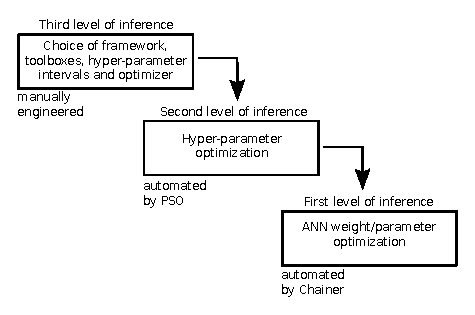
\includegraphics[width=0.7\columnwidth]{modeling/levels_of_opt.eps}
	\caption{The three levels of optimization and in how far they are automated}
	\label{fig:opt_levels}
\end{figure}

%PMSM
\textit{Escalante et. al.} performed an extensive model selection search via \gls{pso} and called it \gls{psms} \cite{EsMo2009}.
They achieved with this strategy high ranks in competitions by finding well-performing models in a full model search denoting a high-dimensional search space without over-fitting and simultaneously incorporating no prior knowledge of the domain.
Although their findings are based solely on binary classification tasks, chances are high, that model selection via \gls{pso} might also prove efficient for regression tasks.

\subsection{Particle Swarm Optimization}
\gls{pso}, originally proposed by \textit{Kennedy and Eberhart} in \cite{KeEb1995}, has its inspiration from natural clusters of biological entities showing individual and social behavior e.g. a bee hive, a school of fish or flocks of birds. Typically all members of the community share a common goal and they attempt to achieve it by exploring their environment individually while also reporting their findings to the society in order to support the overall course of exploration in investigating more promising areas.
The common exploration course is partially random but also slightly dragged to the better found solutions in an iterative manner.
A better site in the search space is defined with respect to a certain error measure representing an at least local optimum.
\gls{pso} is particularly popular because of its simple implementation and competitive performance in return, while computational cost is low as well.
One distinctive feature of \gls{pso} in comparison with evolutionary algorithms is the fact, that no selection is conducted.

The following formulations are based on \cite{Clerc2006}, which should be referred to in order to get a deep understanding of \gls{pso},
though \textit{Clerk's} explanations do not cover the application to hyper-parameters of \glspl{ann}.
The biological entity representatives are called \textit{particles} and all particles represent a \textit{swarm}.
Each particle has a position in the search space and a certain velocity during each time increment or iteration.
After every particle has evaluated the cost function at its position, these information is (partly) propagated through the swarm on which basis movement of each particle is updated.
Typically, the swarm stops after a predefined amount of iterations or until a target value for the cost function is found.
Depending on the update equation, it is also possible for the swarm to converge to a certain site in the search space due to decreasing velocities.

\subsubsection{Swarm Size}
In its simplest version, the number of particles, also called swarm size, is a fixed number.
While \textit{Clerc} states, that swarm sizes between 20 and 40 are sufficient for most problems, \textit{Escalante et. al.} has found during their \gls{psms} that smaller swarm sizes down to even five particles prove feasible \cite{Clerc2006, EsMo2009}.
However, the appropriate number of particles is task-dependent and one cannot infer from their investigations, that a small swarm  size would also be suitable for this thesis' particular task.
As mentioned before, optimizing the hyper-parameters of the hyper-parameter optimization itself (third level of inference) is outside the scope of this work and a swarm size of 100 particles throughout all investigations is applied instead.
Smaller amounts could lead to a global minimum as well, but with a view to the available hardware, which corresponds to a computing cluster, this large swarm size is indeed practicable in the sense of computing time and no risk of too less exploratory power must be taken.

\subsubsection{Initialization}
All particles are randomly initialized in the search space on the whole interval of each hyper-parameter.
Some are distributed uniformly while others are initialized geometrically, that is, randomly in the log domain.
The purpose behind geometrically distributed parameters is the fact, that they influence training in a multiplicative fashion and the same short adjustment has a bigger impact within smaller values than larger ones.

As of the very first iteration, each particle has its own velocity.
Thus, initial velocities are randomly distributed as well.
Distribution strategies are the same as for position initialization but with a bias in the interval towards zero in order to permit negative velocities as well.
The initialization interval for each particle's velocity per hyper-parameter is specifically
\begin{align}
	v_i\in[\frac{-(x_{max} - x_{min})}{2}, \frac{x_{max} - x_{min}}{2}],
\end{align}
with $v_i$ being the velocity of hyper-parameter $i$ and $x_{max}$ and $x_{min}$ denoting the upper and lower bound of the hyper-parameter's interval, respectively.

\subsubsection{Information and Informants}
The evaluation metric for a specific position in the hyper-parameter search space is chosen to be represented by the test set score.
Consequently, evaluating one spot in the search space is connected with the full training of a neural network and the following cross validation with the test set.
This is reasonable insofar, that a set of parameters is only interesting in terms of the resulting neural net's generalization abilities and, hence, the swarm should converge towards this objective.
The disadvantage of this procedure is the fact, that a spot's cost is not directly affected by the hyper-parameters explaining the search space but indirectly through the weights of the trained neural network, which were developed with a sense of randomness during training.
Moreover, the neural network weights are trained on the training set, selected with respect to the validation set performance and the test set score is in turn an independent performance measure.
This independence could give the swarm a blurred understanding of which sites are attractive and which are not.

Another point concerning swarm convergence is the specific implementation of ``social behavior'' or swarm intelligence.
One possible implementation would be the forwarding of each particle's best found position to every other particle such that each particle always knows what spot was the best up to the current iteration.
Nonetheless, this could lead to a biased convergence towards the initial positions and deaden the exploratory character of the swarm.
As an alternative, the global best position can be communicated to a certain particle by a group of informants composed of a number of other particles.
The group of informants for each particle varies randomly, in particular, each group of informants is made up by random other particles in the swarm to a predefined group size at each iteration.
This method resembles the spread of a rumor.
In \cite{Clerc2006} it has been shown, that, by this procedure and having always two informants, each particle has received information from almost definitely every other particle after ten iterations.
Thus, the number of random informants is set to two for all investigations.
Implementing this sort of communicating the global best position, the swarm is encouraged to explore the search space more thoroughly as not every particle acts according to the very same information.
Note, that the group of informants denotes a unidirectional information transfer, that implies, that if a particle knows a better spot than its informants, then they will not get to know that in turn.
In other words, the knowledge about the best global position a certain particle has been communicated to will only leave that particle to another, if that particle becomes an informant for another.

As soon as a spot is evaluated, the corresponding particle will overall hold following information:
\begin{itemize}
	\item its own position in the search space,
	\item this position's cost,
	\item the particle's best visited position in terms of lowest cost and the corresponding evaluation measure (\textit{personal best}) and
	\item the \textit{global best} position in the search space together with that spot's cost, as communicated by the particle's informants up to the current iteration.
\end{itemize}
In the beginning, each particle's personal best and global best is represented by its current position's cost.
If the particle's informants do not know a better site than the particle itself, the particle's global best remains unchanged.

\subsubsection{Velocity Update}
After each iteration, when all particle positions are evaluated, groups of informants are set and all information is transmitted, each particle's velocity is updated according to its current velocity, its personal best position and its global best position.
The update formulas per dimension are as follows:
\begin{align}
	v_i&\gets c_{self}v_i + c_{max}u(p_i - x_i) + c_{max}u(g_i - x_i)\\
	x_i&\gets x_i + v_i
\end{align}
where $x_i$ stands for the position in dimension $i$, $p_i$ and $g_i$ for personal best and global best position, respectively, while $u$ denotes a uniformly random value between $0$ and $1$.
The constant factor $c_{self}$ is similar to a momentum or the particle's confidence in its own velocity, whereas the constant $c_{max}$ represents the maximum confidence in its personal and global best position.
There are several alternatives to this approach imaginable.
Fig. \ref{fig:particle} illustrates how a particle's movement is affected by its displacement to its known personal and global best position.
\begin{figure}
	\centering
	\def\svgwidth{0.7\columnwidth}
         \import{eps/modeling/out/}{vel_update.pdf_tex}
         \caption{The basic displacement update for particles according to their best known sites}
         \label{fig:particle}
\end{figure}

Furthermore, the choice of the constant factors is made upon the recommendations in \cite{Clerc2006}, that are, $c_{self}= 0.7$ and $c_{max}= 1.43$.
These selections decrease velocities on average and the swarm is more likely to converge.

In addition, there is an off-bounds check in order to bring particles back to the hypercube defining the valid search space.
The heuristic here is to put the particle's position back to the upper or lower bound of the specific dimension that has been exceeded and to reset its velocity to zero.
Its subsequent velocity is then determined by its displacement to its personal and global best only, after which the particle would have an own velocity again.

The swarm is exploring the search space as long as the maximum number of iterations is not reached or until a predefined cost objective is found or until the swarm converges.
Here, the values are set to 100 iterations at maximum and a goal of less than \SI{1}{\kelvin\squared} in the \gls{mse} cost of the test score.
%What kind of PSO? Parametric or Non-Parametric(adaptive)? How many swarms?
%parallel computing rather than sequential, because one evaluation is long.

\subsection{Search Space}
In this work, the hyper-parameter search space consists of 15 dimensions, each limited to a specific predefined interval.
While continuous hyper-parameters, such as initial learn rate, are intuitively applied to the \gls{pso} search space, discrete parameters e.g. number of hidden layers and mutually exclusive choices as the optimizer technique need to be mapped onto a continuous interval coding in order to give a particle's velocity meaning there.

Tab. \ref{tab:hyperparams} shows an overview of the incorporated hyper-parameters.
Abbreviations for the hyper-parameter names are stated aside if given and are used during the remainder of the work for convenience.
Note, that some hyper-paramaters become active only in combination with certain choices in other hyper-parameters e.g. `PCA variance' has an effect only if `normalization' is set to `PCA'.

\begin{table}
	\rarray{1.3}
	\caption{A list of those hyper-parameters explaining the search space for the \gls{pso}}
	\label{tab:hyperparams}
	\centering
	\begin{tabular}{C{4.5cm} C{4cm} C{5cm}}
		\toprule
		hyper-parameter name & interval discretization & interval bounds/ choices\\
		\midrule
		architecture (arch)& mutually exclusive & \gls{lstm}, \gls{lstm} with peepholes or \gls{gru}\\
		number of hidden layers (n\_hl)& discrete & $[1, 3]$\\
		number of units per layer (n\_units)& discrete (log) & $[2, 256]$\\
		weight initialization - \quad distribution heuristic  & mutually exclusive & unit normal or uniform\\
		weight initialization - scaling heuristic & mutually exclusive & normalized or standard\\
		subsequence length (seq\_len)& discrete & $[30, 7880]$\\
		normalization (preprocess)& mutually exclusive & standard or \gls{pca}\\
		PCA variance (pca\_var)& continuous & $[0.5, 1.0]$\\
		lookback & discrete & $[0, 2000]$\\
		optimizer (opt)& mutually exclusive & \gls{adam}, Nesterov or \gls{sgd}\\
		initial learn rate (lr\_init) $\eta$& continuous (log) & $[1\cdot 10^{-4}, 1\cdot 10^{-1}]$\\
		learn rate decay factor (lr\_decay) $\alpha_d$ & continuous & $[0.5, 0.99]$\\
		regularization (active)& binary & $[0, 3]$\\
		gaussian noise $\sigma$ & continuous (log) & $[1\cdot 10^{-7}, 1\cdot 10^{-3}]$\\
		weight decay $\lambda$& continuous (log) & $[1\cdot 10^{-7}, 1\cdot 10^{-4}]$\\
		\bottomrule
	 \end{tabular}
\end{table}
The architecture parameter determines which memory block to choose (\gls{lstm}, with or without peepholes, or \gls{gru}; see sec. \ref{sec:arch}).

Number of hidden layers varies between one and three, while number of neurons per layer ranges from two to 256.
Intermediate experiments have been conducted with maximum number of layers at five and maximum number of units at 128, but the best models always certainly stayed at one layer and had their units near the upper bound such that these limits have been adjusted for the final experiments.
 
Weight initialization distribution and scaling were varied according to the heuristics explained in sec. \ref{ssec:init}.
The subsequence length is limited to at least 30 time-steps and at most the full length of the shortest profile in the training set.
Normalization was performed either with or without \gls{pca}, whose dimensionality reduction would have been utilized by keeping a variance between 50\% and 100\%.
The lookback parameter describes the amount of time-steps in the past, that are considered for enriching the input data with the first and second stochastic moments of each input parameter.
The selected optimizer was either \gls{adam}, Nesterov-style momentum or standard \gls{sgd}.
The initial learn rate is set geometrically, while learn rate decay is set uniformly.
The binary ``regularization'' parameter determines whether both, one or none of the two regularization techniques are applied.
In particular, ``zero'' equals to ``no regularization''; ``one'' to ``gaussian noise only''; ``two'' to ``weight decay only'' and ``three'' sets both regularization techniques active.
Gaussian noise on gradients has its standard deviation applied randomly while weight decay is determined by its penalty factor $\lambda$.


    \chapter{Evaluation} 
\label{cha:evaluation}
Following the model strategy defined in the previous chapter, all model learning and evaluation scripts were run on a computing cluster, the \gls{pc2}.
Several \glspl{pso} were conducted, each with a different target to optimize for.
During every swarm iteration, computational requirements for each model and its hyper-parameters are set heuristically according to those parameters having a significant impact on the optimal training time and on allocatable resources.
The neural network framework Chainer comes with a built-in parallelization mechanism on CPU and GPU level and hence the only challenge here is to find the optimal amount of resources and allocation time without neither having the model training to starve on its supplement nor running on not utilizable capabilities.
In view of the long simulation time of multiple \glspl{pso}, it is advantageous to be able to reduce waiting time for reserved resources by adapting the reservation on the probably incurring demand.

It has been found, that the following parameters determine most of the demand:
\begin{itemize}
	\item number of hidden layers,
	\item number of units per hidden layer and
	\item subsequence length.
\end{itemize}
Consequently, resource requirements were calculated in accordance with these parameters.

Overall, all conducted hyper-parameter optimizations encompass the training and evaluation of 30600 \glspl{ann}.
Results are reported for six experiments: 
\begin{enumerate}
	\item Random search for neural nets modeling all four target temperature.
	\item \gls{pso} for models learning the three stator temperatures without the permanent magnet temperature located in the rotor.
	\item \gls{pso} for models learning to predict permanent magnet temperature $\vartheta_{PM}$.
	\item \gls{pso} for models learning to predict stator yoke temperature $\vartheta_{SY}$.
	\item \gls{pso} for models learning to predict stator teeth temperature $\vartheta_{ST}$.
	\item \gls{pso} for models learning to predict stator winding temperature $\vartheta_{SW}$.
\end{enumerate}

Though the maximum number of iterations for each swarm were predefined to 100, all experiments converged much earlier, whereas convergence was defined similar to the conditions set for a single \gls{ann} training, that is, if the best model was found in the first half of all iterations after at least 40 iterations.
The maximum time given to each model for learning was limited to two to six hours and the maximum reserved number of CPUs was set to two to six as well.

\section{Optimal Hyper-Parameters}
Every \gls{pso} took a different amount of time to converge, which has plenty of reasons: 
first, different amounts of allocated resources and traffic on the computing cluster can shift the starting time of each model's training indeterminably.
Each iteration submits all of its 100 particles at once, but allocation is dependent on calculated resources and available, unreserved hardware.
Each iteration can go on to the next only if each particle has stopped training and has been evaluated because of the velocity updates being dependent on other particles' best found sites.
There might be iterations facilitating 99 particles at once for two hours, but there is one particle being allocated after these two hours, that needs six hours in turn and prolongs that iteration drastically.

Secondly and obviously, each neural network converges after an unforeseeable amount of epochs.
There could be a hyper-parameter set, that would usually need four hours on average to converge but specific weight initializations and a fortunate path during gradient descent may bring training to an end in under an hour.

Furthermore, different hyper-parameter sets exhibit different challenges for training such that training time is affected a priori by the parameter selection or, respectively, the particle's position in the search space.

\subsection{Precision of Estimation}
Tab. \ref{tab:optimum_performance} summarizes the best found performances on the test set ordered by the swarms' target.
The mean test score describes the performance of that model holding the best mean test score of all its targets, while individual test scores are reported for different models within the experiment achieving the best test score for that specific target.
Number of iterations explains the overall conducted iterations, though the best models were found earlier - usually in the first half of iterations.
\begin{table}
	\caption{Best found performances in all experiments.
	 While experiment 1 denotes a random search, experiment 2-6 are conducted by \gls{pso}.}
	\label{tab:optimum_performance}
	\centering\rarray{1.4}
	\begin{tabular}{ c  C{2cm}  C{1.5cm}  C{2cm} C{3cm}  C{4cm}}
		\toprule
		 no. & target & number of iterations &  mean test score in K\textsuperscript{2} & mean validation score in K\textsuperscript{2}  & individual test score in K\textsuperscript{2}\\
		 \midrule
		 1& $\vartheta_{PM}$, $\vartheta_{SY}$, $\vartheta_{ST}$, $\vartheta_{SW}$ & 52\newline 16 days & 24.05 &22.18 & $\vartheta_{PM}$:\,50.61; $\vartheta_{SY}$:\,4.78 $\vartheta_{ST}$:\,9.28; $\vartheta_{SW}$:\,17.56\\
		 2& $\vartheta_{SY}$, $\vartheta_{ST}$, $\vartheta_{SW}$ & 68\newline 21 days& 5.1 & 6.99 & $\vartheta_{SY}$:\,1.46;  $\vartheta_{ST}$:\,3.64 $\vartheta_{SW}$:\,8.01 \\
		 3& $\vartheta_{PM}$ & 40\newline 14 days& 13.55  & 19.17 & \quad\\
		 4& $\vartheta_{SY}$ & 46\newline 17 days & 2.38 & 1.24 & \quad\\
		 5& $\vartheta_{ST}$ & 42\newline 11 days& 5.49  & 6.48& \quad\\
		 6& $\vartheta_{SW}$ & 58\newline 11 days & 9.44  & 6.34& \quad\\
		  \bottomrule
	\end{tabular}
\end{table}

An important finding here is the fact, that the stator yoke temperature is always predicted most precisely, followed by the stator teeth temperature and the stator winding temperature, whereas permanent magnet temperature is modeled poorly.
The first explanation for the varying performances within the multi-target experiments could be, that undoing the normalization of the target predictions results in different distances between prediction and groundtruth due to the targets' different standard deviation.
Yet the permanent magnet standard deviation is not larger than that of the stator teeth and the single-target experiments' relative performance to each other show resemblance with the proportions of the multi-target experiments' predictions.
Hence, the drawback of normalization does not seem to harm neural networks predicting multiple targets and modeling them can be recommended without having to put up with trade-offs.
Furthermore, the difficulty of predicting the temperature in the rotor might be higher than that for the stator temperatures.

More interestingly, experiment 2 has found better predictions than the single-target neural networks in experiments 4-6.
This indicates, that experiment 2 must have found a better local optimum, if not even the global optimum, than the other three experiments had, although \gls{pso} was thought of being able to track the global optimum robustly.
This gives rise to the consistency tests further in this chapter.
Not shown in tab. \ref{tab:optimum_performance} but moreover indicating the fact of the better found optimum, the individual scores of the second experiments' model holding the best mean score still show better performance than that of the single-target experiments.  

The best prediction for each target temperature is illustrated in fig. \ref{fig:best_predictions}.
Permanent magnet prediction is taken from experiment 3, while the stator temperature estimates originate from experiment 2 and there from two distinct models.

\begin{figure}[!htb]
	\centering
	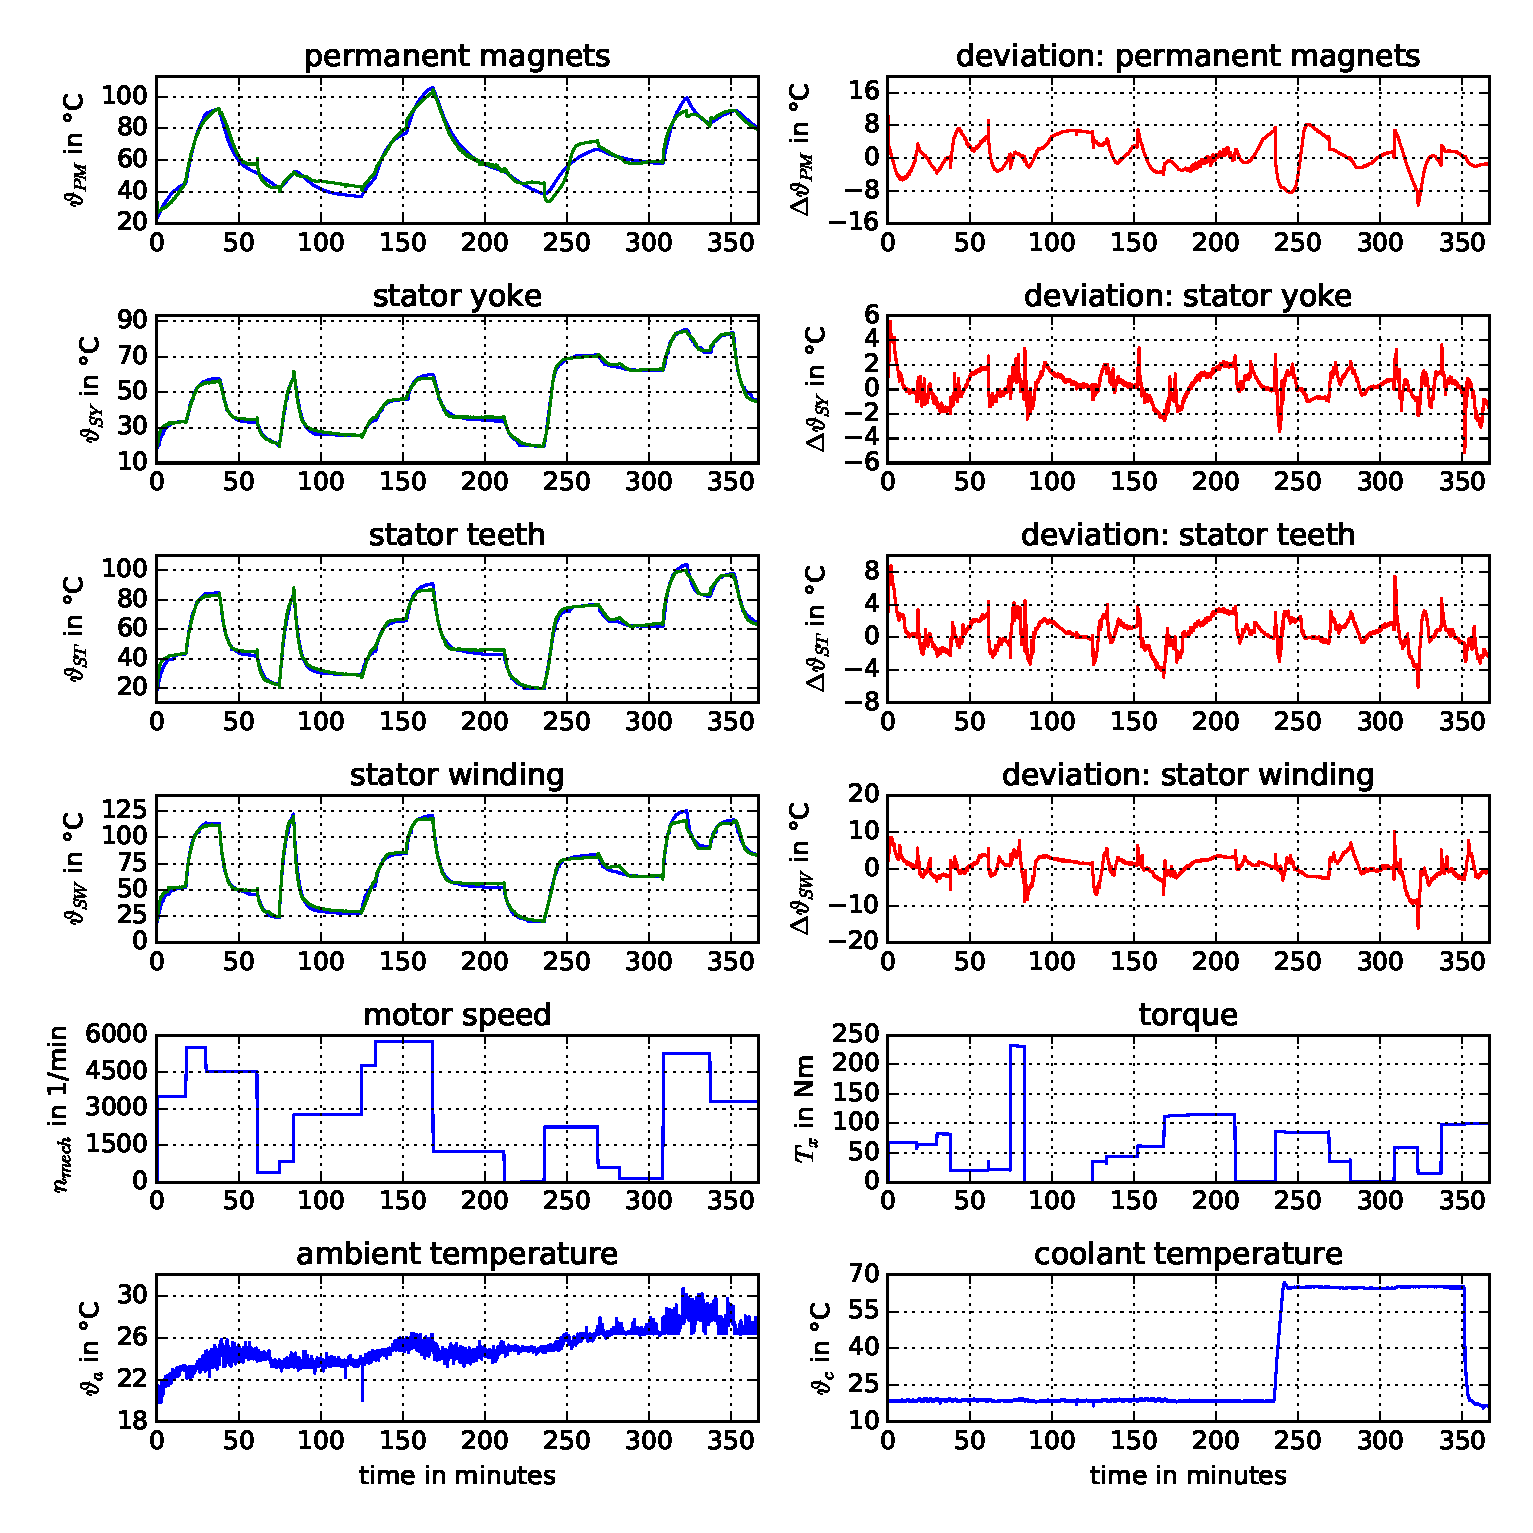
\includegraphics[width=\columnwidth]{evaluation/alltargets_test.eps}
	
	\caption{Cross-validation on the test subset (blue = measured groundtruth, green = prediction, red = deviation)}
	\label{fig:best_predictions}
\end{figure}

Here, the main finding from tab. \ref{tab:optimum_performance} is illustrated and confirmed again:
the permanent magnet temperature is obviously predicted poorly, while the stator temperatures were modeled decent.
One can infer from these plots, that neural networks seem to have trouble modeling the exponential rise and fall in the time series.
The largest distances between prediction and groundtruth happen when the prediction ceases following the exponential curves and stagnates to a plateau.

Comparing the prediction accuracy with those of \glspl{lptn} (see \cite{WaBo2016}), the achieved performance is similar, though during some time periods the worst-case deviation of permanent magnets and stator winding prediction dramatically exceeds that of \gls{lptn} estimates.

\subsection{Optimal Sets}
The particular choices of hyper-parameters for the optimum in each experiment are outlined in tab. \ref{tab:optimum_choices}.
\begin{sidewaystable}
	\caption{Hyper-parameter sets of the optima found in each experiment}
	\label{tab:optimum_choices}
	\centering\rarray{1.4}
	\begin{tabular}{c c c c c c c}
		\toprule
		 \quad & \multicolumn{6}{c}{experiment no.}\\
		 hyper-parameter & 1 & 2 & 3 & 4 & 5 & 6\\
		 \midrule
		 arch & \gls{lstm} & \gls{gru} & \gls{gru} & \gls{gru} & \gls{gru} & \gls{gru}\\
		 n\_hl & 1 & 1 & 1 & 1 & 1 & 1\\
		 n\_units & 35 & 122 & 143 & 236 & 115 & 38\\
		 weight init. distribution & unit normal & unit normal & unit normal & unit normal & unit normal & unit normal\\
		 weight init. scaling & normalized & normalized & normalized & standard & standard & normalized\\
		 seq\_len & 7800 & 7292 & 7880 & 862 & 360 & 6670\\
		 preprocess & standard & standard & standard & standard & standard & standard\\
		 pca\_var & 0.55 & 0.8 & 0.71 & 0.86 & 0.73 & 0.88\\
		 lookback & 937 & 822 & 2000 & 1060 & 880 & 732\\
		 opt & nesterov & adam & adam & adam & adam & adam\\
		 lr\_init & \num{1e-4} & 0.0172 & 0.0125 & 0.0112 & 0.0022 & 0.0217\\
		 lr\_decay & 0.98 & 0.97 & 0.95 & 0.9 & 0.79 & 0.66\\
		 active regularization & 3 & 1 & 1 & 2 & 2 & 2\\
		 gaussian noise & \num{1e-3} & \num{2.92e-5} & \num{1.54e-5} & \num{3.21e-4} & \num{3.82e-6} & \num{1.57e-4}\\
		 weight decay & \num{1e-4} & \num{7.23e-5} & \num{3.28e-5} & \num{1.55e-6} & \num{2.17e-6} & \num{2.22e-5}\\
		 \bottomrule
	\end{tabular}
\end{sidewaystable}

There are plenty of insights one can infer from the found optima.
First of all, homogeneously across all experiments, \gls{gru} with one hidden layer seems to be the optimal architecture; a unit normal weight initialization distribution appears being better than a uniform distribution; \gls{pca} is not improving performance over standard normalization and, as expected, Adam is the preferred optimizing technique.

The reason for \gls{gru} performing better than its counterparts might be its fewer adjustable weights, hence, it is less prone to over-fitting.
This thesis is further emphasized by the \gls{lstm} with peepholes having the worst scores and the highest number of weights to train.

The fact, that one hidden layer beats multiple might be due to the simplicity in the regression problem with respect to other problems in the real world, where deeper nets always perform better.
On the other hand, this optimum also might be caused by having too less training time allocated to the nets, though surveying the training trends for models with higher amounts of hidden layers reveals convergence most of the time.

Differences regarding the architecture are exhibited for the number of units.
Modeling the stator yoke demands a large amount of 236 units, while stator winding modeling requires mere 38 units.
This is a strong indicator for the different \gls{pso} durations, as shown in tab. \ref{tab:optimum_performance}.

Another interesting difference, especially between single target swarms, is evident in the subsequence lengths.
While permanent magnet temperatures need the maximum amount (7880 time steps) of comprehensive sequences, which suggests to drop the subsequences-strategy, stator winding temperatures can cope with around 6700 time steps and the other two stator temperatures are even satisfied with under 900 time steps, minimum at 360 time steps for experiment 5.
This evidences, that stator temperature regression in this particular task does benefit from the specially engineered subsequences-strategy, albeit this is not the case for the rotor temperature.

The necessity of long comprehensive sequences in case of permanent magnets becomes even more clear when examining the lookback optimum, which also points on the maximum length, whereby half of it suffices for stator temperatures.
As a reminder, saving statistical moments of certain time sequences poses infeasible memory requirements for automotive applications today.
Omitting these additional input quantities can be compensated by having more data as a basis for training.
Hence, the demand for long past sequences simultaneously constitutes the demand for more benchmark data.

The remaining differences in optimal hyper-parameter selection across the experiments are minor and their latent impact on performance is more thoroughly investigated in sec. \ref{sec:relevance}.

\subsection{Swarm Convergence}
Regarding the \glspl{pso}, sanity checks consisting of velocity monitoring and evaluation distribution as well as global best progress were executed.
Fig. \ref{fig:velocity} depicts how fast particles decelerate over all iterations upon the example of experiment 2.
Here, the mean absolute velocity of a particle is calculated by dividing the absolute velocity of each particle's dimension by the dimension's interval, summing all dimensions up and dividing again by the number of hyper-parameters, that is, by 15.
The velocity trend of the other experiments is very similar (see app. \ref{app:velocity}).

It becomes evident, that each swarm's particles slow down over time and converge to a certain spot in the search space.
This is the expected behavior since the velocity update formula has an expected mean at $E[c_{max}u] = 0.7$ for $c_{max} = 1.4$.  
% velocity convergence plot
\begin{figure}
	\centering
	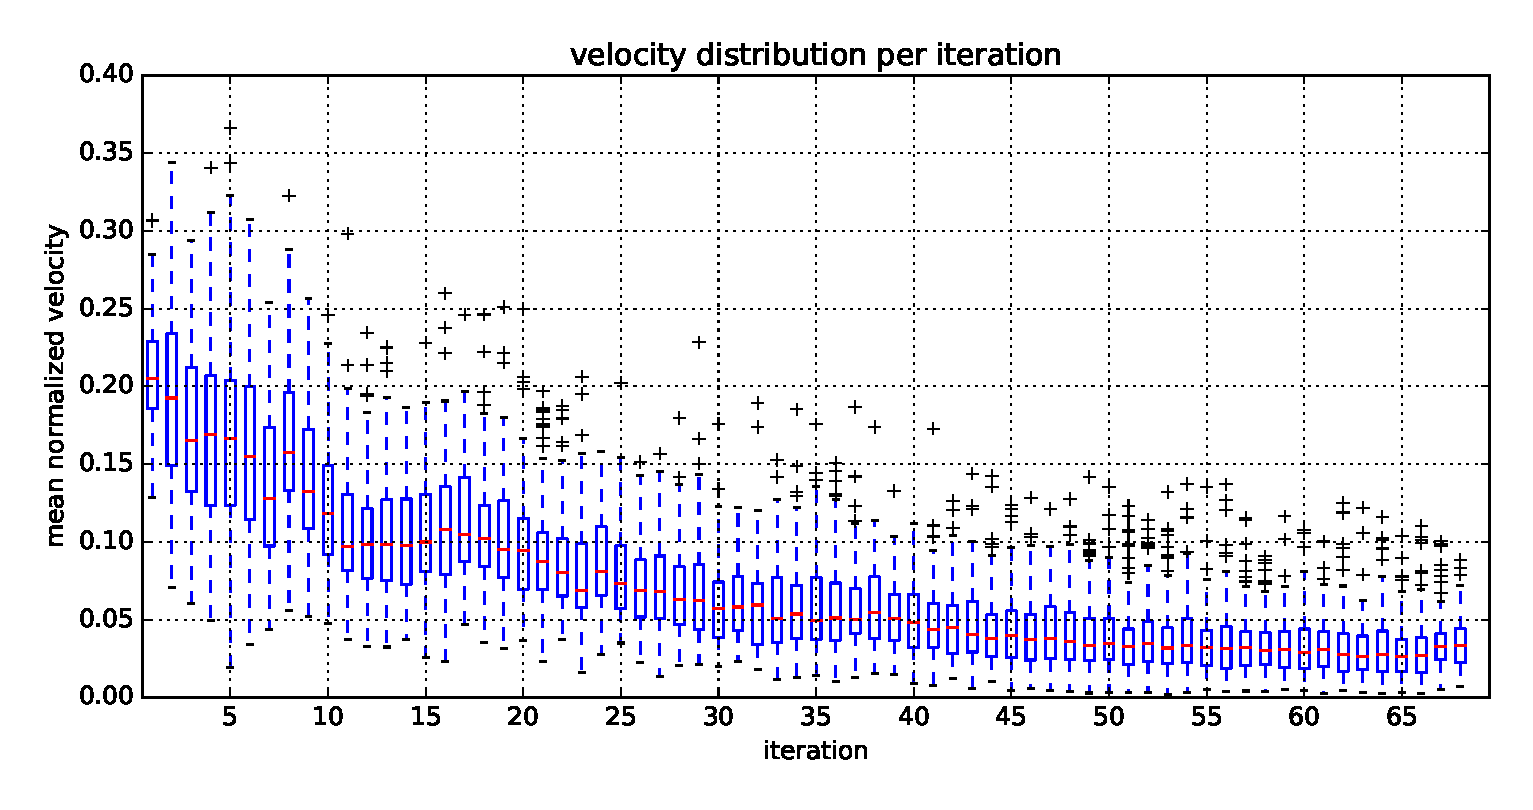
\includegraphics[width=\columnwidth]{evaluation/stator_vel.eps}
	\caption{Mean absolute velocity of the swarm's particles (from experiment 2)}
	\label{fig:velocity}
\end{figure}

% Evaluation distribution and gbest progress
In order to evaluate a swarm's performance, each particle's test score is displayed over the entirety of iterations in fig. \ref{fig:evaluation_development}, again, upon the example of experiment 2.
The global best progress is illustrated aside for better comparability.
The other experiments' trends show strong resemblance with fig. \ref{fig:evaluation_development} (see app. \ref{app:evaluation}).

% Describe what is seen in these plots
Fig. \ref{fig:evaluation_development} shows, that, up to a certain iteration, performance is not improving significantly anymore.
Moreover, the global best model is determined by lower outliers evaluated at apparently the same site in the search space.
This is indicated by the median of the particle test errors (the red mark) being at around the same performance level while the global best is still improving.
Assuming that as of the second half of iterations the same search space position's proximity is explored over and over again, one can infer from the broad scatter that the evaluation of a specific site comes with a broad variance as well.
\begin{figure}
	\centering
	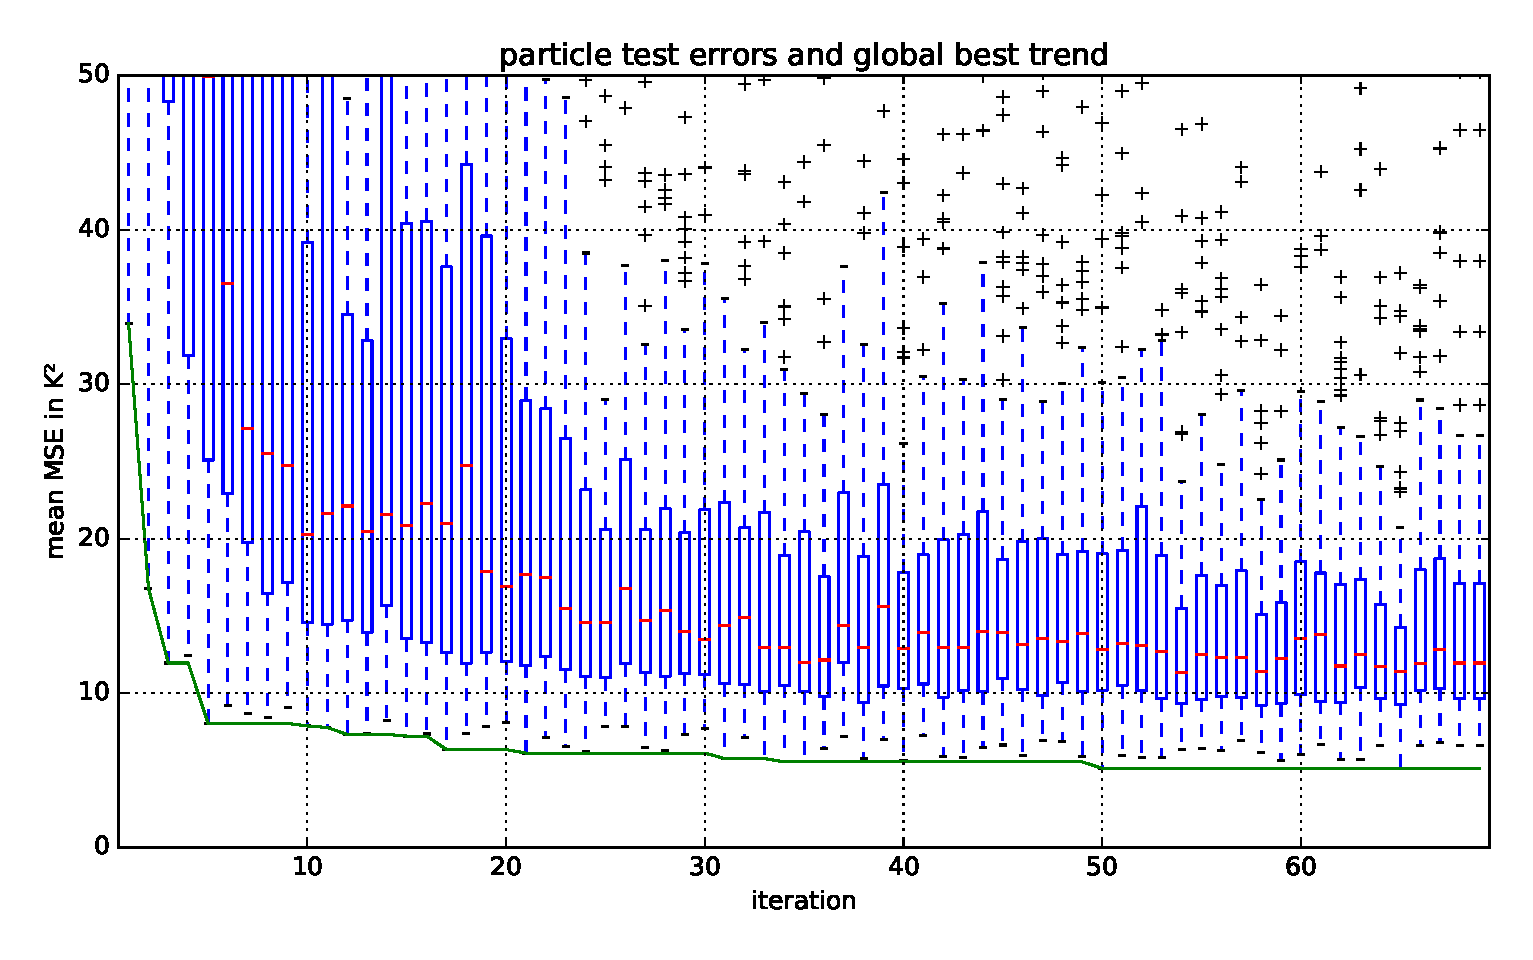
\includegraphics[width=\columnwidth]{evaluation/stator_eval.eps}
	\caption{Particle test scores over all iterations as box plots and the found best site's score as green line (from experiment 2)}
	\label{fig:evaluation_development}
\end{figure}

\subsection{Consistency}
In order to investigate the scatter of the optimal sites of each experiment, their optimal hyper-parameter sets were utilized for further 50 to 100 evaluations.
The resulting sample should give a clear insight to the mean performance and the standard deviation of the underlying hyper-parameters.

Fig. \ref{fig:consistency} depicts the scatter of the optimal hyper-parameters as histograms.
Outliers were removed, whereas an outlier is detected as such, if it has a score beyond 2.5 times the sample standard deviation.
Having outliers removed, a more robust sample standard deviation can be calculated.
The resulting sample means and standard deviations are stated in tab. \ref{tab:consistency}.

% consistency
%all targets: $\sigma = 4.55 K^2$. 15 samples zu $\pm 2.3 K^2$.
%stator: $\sigma=5 K^2$. 15 samples zu $\pm 2.53 K^2$.
%pm: $\sigma=13 K^2$. 73 samples zu $\pm 2.98 K^2$
%yoke: $\sigma=4.25$. 15 samples zu $\pm 2.15 K^2$.
%teeth: $\sigma=4.39$. 15 samples zu $\pm 2.22 K^2$.
%winding: $\sigma=5.57$ 15 samples zu $\pm 2.82 K ^2$.
\begin{figure}[!tbh]
	\centering
	\begin{subfigure}{0.31\textwidth}
		\includegraphics[width=\columnwidth]{evaluation/alltargets_consistency.eps}
		\caption{experiment 1 optimum}
	\end{subfigure}
	~
	\begin{subfigure}{0.31\textwidth}
		\includegraphics[width=\columnwidth]{evaluation/stator_consistency.eps}
		\caption{experiment 2 optimum}
	\end{subfigure}
	~
	\begin{subfigure}{0.31\textwidth}
		\includegraphics[width=\columnwidth]{evaluation/pm_consistency.eps}
		\caption{experiment 3 optimum}
	\end{subfigure}
	
	\begin{subfigure}{0.31\textwidth}
		\includegraphics[width=\columnwidth]{evaluation/yoke_consistency.eps}
		\caption{experiment 4 optimum}
	\end{subfigure}
	~
	\begin{subfigure}{0.31\textwidth}
		\includegraphics[width=\columnwidth]{evaluation/teeth_consistency.eps}
		\caption{experiment 5 optimum}
	\end{subfigure}
	~
	\begin{subfigure}{0.31\textwidth}
		\includegraphics[width=\columnwidth]{evaluation/winding_consistency.eps}
		\caption{experiment 6 optimum}
	\end{subfigure}
	\caption{Consistency tests showing histograms of the optimal hyper-parameters evaluated repetitively. Mean score of single-target experiments corresponds to the individual single target score.}
	\label{fig:consistency}
\end{figure}
\begin{table}[h]
	\caption{Sample characteristics for each consistency test}
	\label{tab:consistency}
	\centering
	\begin{tabular}{ c C{2cm} C{2cm} C{3cm} C{3cm}}
		\toprule
		 no. & $\mu$ (test)\quad in K\textsuperscript{2}& $\sigma$ (test)\quad in K\textsuperscript{2}&$\mu$ (validation)\quad in K\textsuperscript{2}& $\sigma$ (validation)\quad in K\textsuperscript{2}\\
		 \midrule
		 1& 33.16 & 4.54 & 48.07 & 2.39\\
		 2& 12.11 & 5.04 & 16.42 & 2.37\\
		 3& 38.41 & 13.02 & 56.42 & 8.19\\
		 4& 7.8 & 4.25 & 9.1 & 1.03\\
		 5& 12.41 & 4.39 & 24.51 & 2.57\\
		 6& 21.53 & 5.57 & 38.41 & 4.08\\
		  \bottomrule
	\end{tabular}
\end{table}

It becomes clear from fig. \ref{fig:consistency} and tab. \ref{tab:consistency}, that there is a large scatter inherent in every search space site's evaluation and that the best performances are critical outliers of that specific position.
Although the hyper-parameters are set constant, the evaluation on the test set cannot be stated unambiguously by a mere single evaluation, as it was conducted during this work's experiments, but rather by the mean of multiple evaluations, that would vary within a certain significance interval to a given chance (usually 95\,\%).
For instance, assuming the standard deviation estimate from the consistency tests represents the true standard deviation sufficiently, one would have to execute 15 evaluations of a single spot in order to be able to declare this sample's mean to be in an interval length of under 6\,K\textsuperscript{2} with a 95\,\% chance.
This is the case for all experiments except for experiment 3, which has its standard deviation estimate at around 13\,K\textsuperscript{2} instead of approx. 5\,K\textsuperscript{2}.
Unfortunately, that would also mean to have the experiment duration increased fifteenfold, which slingshots the \gls{pso} to infeasibility.
In case of experiment 3, even 73 evaluations were required.

The reason for the large scatter is undoubtedly rooted in the random weight initialization since gradient descent training is very sensitive to its initial starting point in the error landscape.
One could go ahead and set a constant seed to the random number generators, but that would only ensure reproducibility and the investigation's exploratory character were sapped.

However, facing these facts, the found optima cannot be declared reliably best in terms of performing best on the test set on average, yet they surely are close to optimal sets as numerous particles were tempted to find a global optimum.
Furthermore, the obtained results give a fair insight to what extent neural networks are capable of modeling important component temperatures inside \glspl{pmsm}.

\section{Hyper-Parameter Relevance}
\label{sec:relevance}
Having determined close to optimal hyper-parameters for each target, one is interested in how far each hyper-parameter is important for a decent modeling.
If it is possible to track those parameters having no impact on the modeling performance, then future investigations could concentrate on less or other input measures.

\subsection{Scatter Over PSO Iterations}
% parameter distribution
Before an extensive sensitivity analysis is conducted, the specific choice of hyper-parameters over all iterations are investigated first.
Since the coarse global optimum site in the search space is presumably found early on, most of the choices should be distributed on the optimal choices.
Hyper-parameters, which are more or less uniformly distributed over their full interval, were likely changing their global best value frequently together with the global optimum progress.
This indicates, that those hyper-parameters were not of much relevance, since completely different values were found to be the very best more often.
Conversely, if a hyper-parameter is distributed narrowly around a certain value, then this value was probably found to be the best relatively early without fail during later transitions of the global optimum.

Fig. \ref{fig:param_dist} presents the distribution of all hyper-parameters over the entirety of iterations in experiment 4.
The remaining distribution plots are attached to app. \ref{app:param_dist}.
\begin{figure}[!bth]
	\centering
	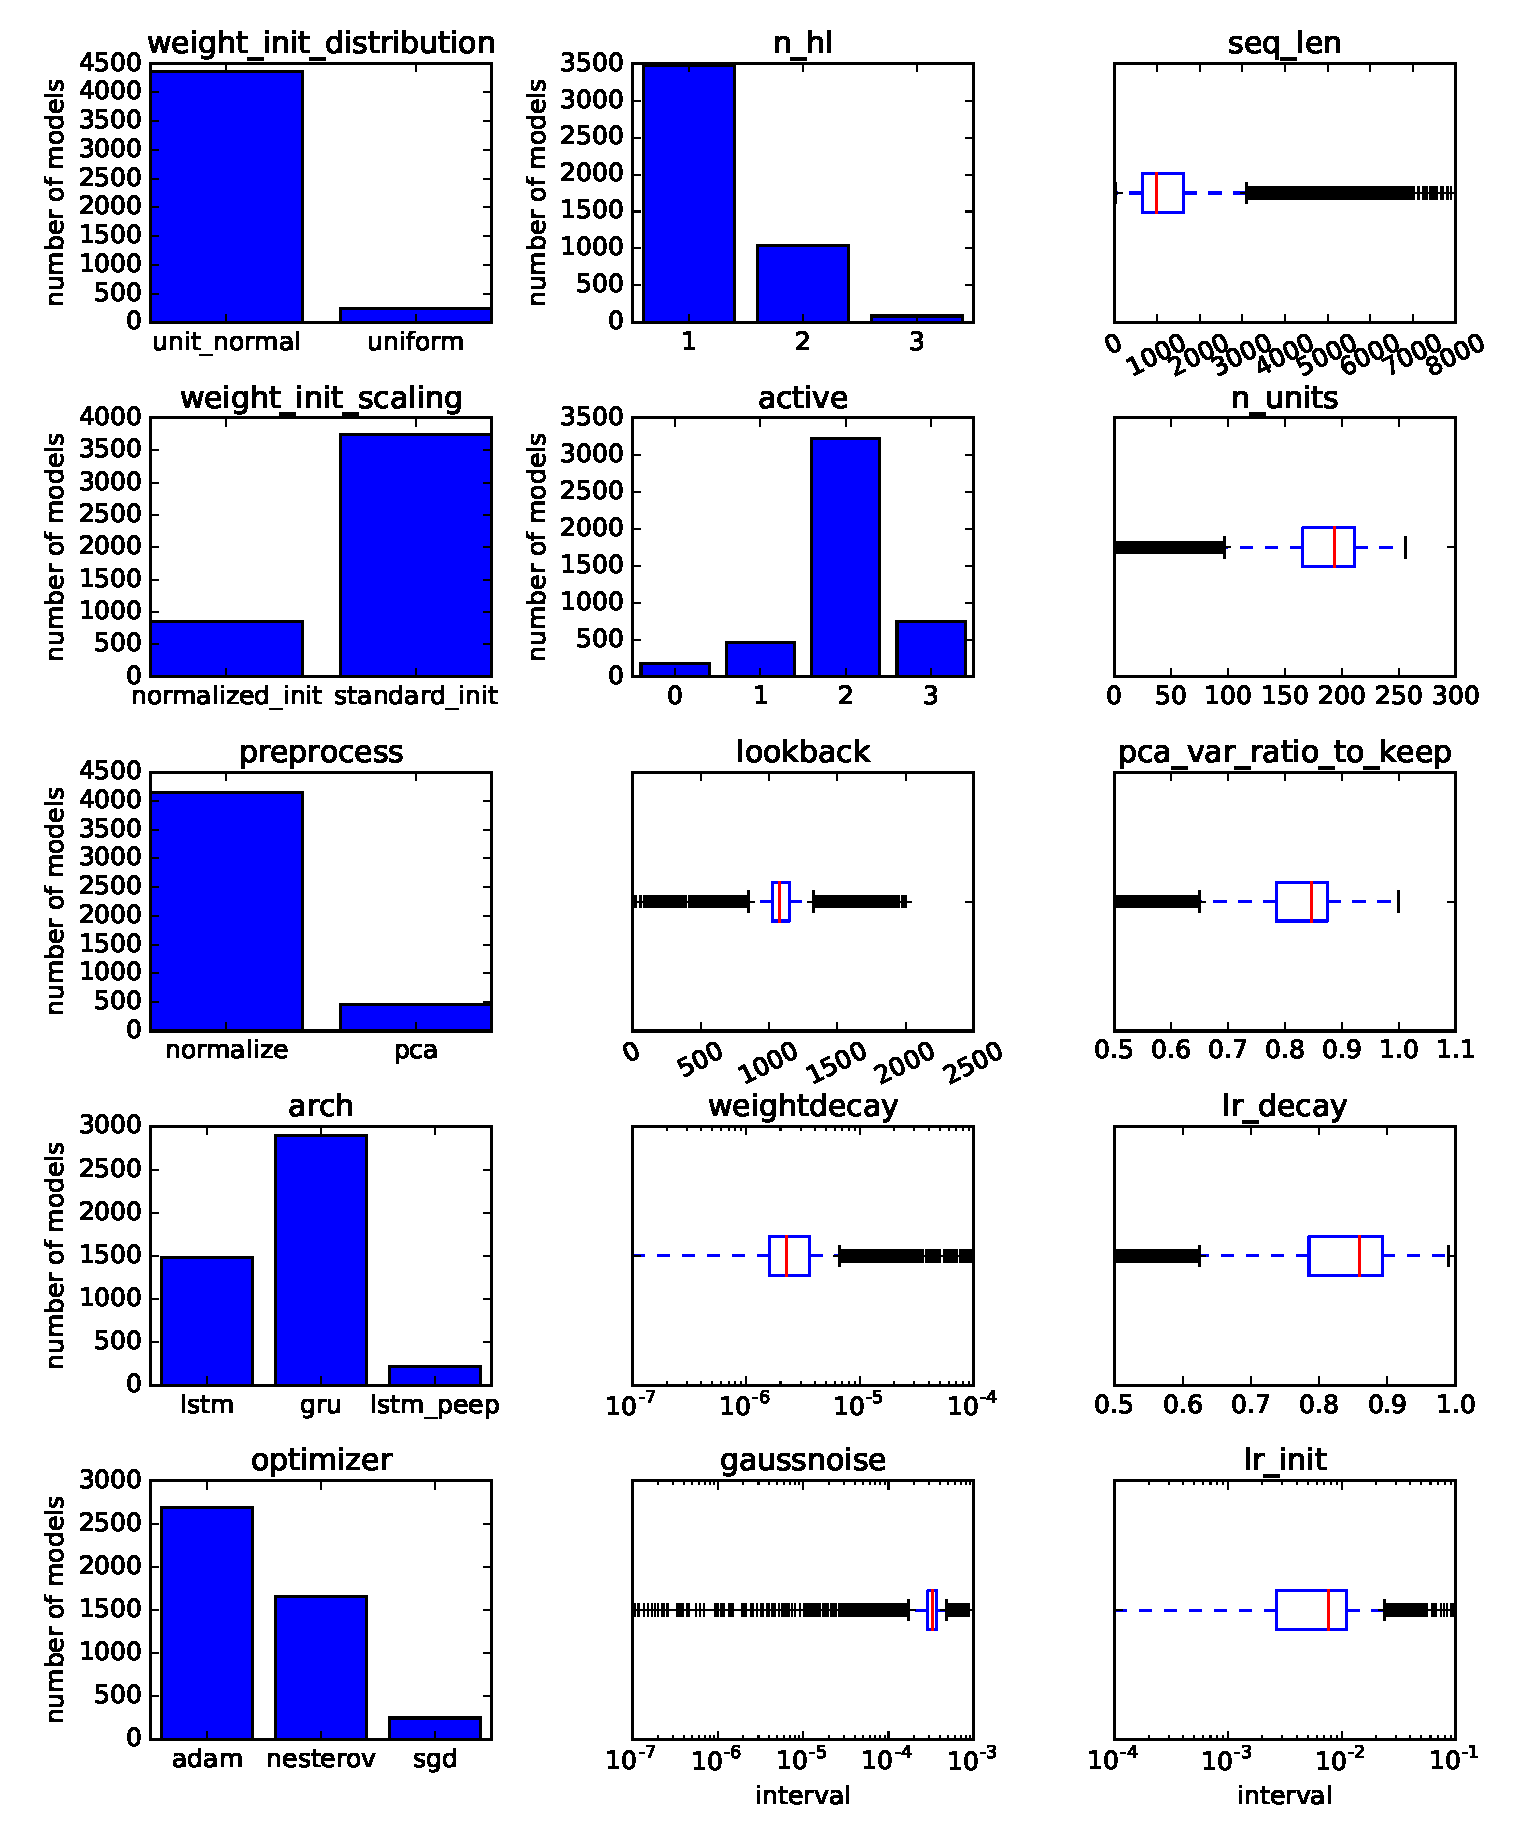
\includegraphics[width=\columnwidth]{evaluation/yoke_paramdist.eps}
	\caption{Bar plots and box plots depicting the distribution of each hyper-parameter over all \gls{pso} iterations (from experiment 4)}
	\label{fig:param_dist}
\end{figure}

Comparing the distributions in fig. \ref{fig:param_dist} with the optimal values of experiment 4 in tab. \ref{tab:optimum_choices}, it becomes clear, that the vast bulk of choices are indeed set around the optimum.
The same situation is observable for the other distribution plots in app. \ref{app:param_dist}.
This hint underlines the thesis, that during the whole \gls{pso}, the global best site's proximity is more thoroughly explored than other sites.

Now for the very case of experiment 4, it becomes evident, that some parameter distributions are more spiked around the optimum than others.
The lookback value, for instance, is relatively narrowly distributed, while learn rate decay or number of units is scattered broadly.
This might give a clue about their relevance, as narrowly distributed parameters could tend to exhibit higher sensitivity with respect to model performance than those being flat on the interval.

To summarize what can be found across the board, it can be reliably stated, that obviously concentrated and simultaneously identical distributions are presented by the weight initialization distribution, number of hidden layers, preprocessing variant and architecture.
Regarding the optimizer technique, the stator-yoke-targeted model is the only one, which holds a respectable amount of choices for Nesterov next to \gls{adam}, while all other experiments are almost exclusively attracted to Adam. 
The weight initialization scaling and lookback are also in a peaked shape, but various across experiments.
The other hyper-parameters are widely spread over their interval for at least one experiment.

Unfortunately, there is nothing, that can be inferred from the \gls{pca} variance hyper-parameter distribution as it is practically never applied according to the preprocess hyper-parameter, which sticks to all-standard normalization rather than \gls{pca}.

In order to complement the findings from the parameter distribution plots, the unit interval variances of each hyper-parameter over \gls{pso} iterations are illustrated as well.
Fig. \ref{fig:param_var} depicts that trend for experiment 4.
Hyper-parameters with few alternatives are drawn with solid lines, while the rest is assigned dashed lines.
Those hyper-parameters with a logarithmic scale (see distribution plots) have their unit variance evaluated on the logarithmic scale either.
The hyper-parameter unit interval variances plots for the remaining experiments are attached to app. \ref{app:param_var}.

\begin{figure}[!tbh]
	\centering
	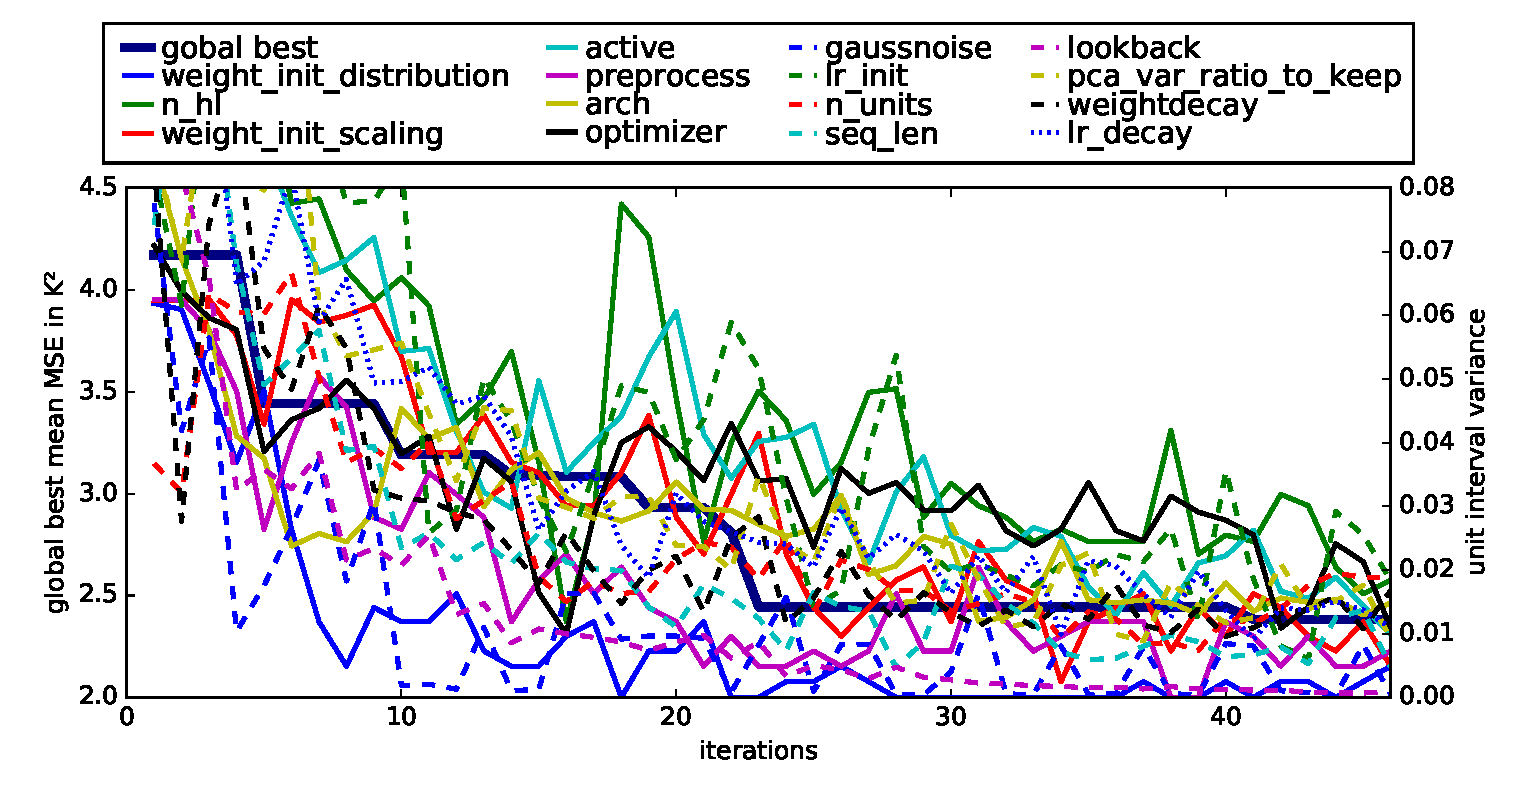
\includegraphics[width=\textwidth]{evaluation/yoke_var.eps}
	\caption{Hyper-parameter variance over \gls{pso} iterations (from experiment 4)}
	\label{fig:param_var}
\end{figure}

One can infer from the variance trends, that those hyper-parameters, that are of a peaked shape in the distribution plots, also show low variance during most of the \gls{pso} iterations.
Consequently, if narrowly distributed parameters inherit high relevance for model performance, it is plausible for them to have a low variance early on or in the progress of the \gls{pso}.
A high sensitivity of the model to low-varying hyper-parameters would be the conclusion, which is to be proven in the next subsection.
Note, that the unit variances calculated here heavily depend on the predefined interval, in which the hyper-parameter was moving.
It is also worth mentioning, that regularization techniques' variance or \gls{pca} variance trends are difficult to interpret, as their corresponding activation parameters ( `active' and `preprocess') were likely to cut them off.

Fig. \ref{fig:param_var} suggests, that for the case of experiment 4 the parameters `lookback', `preprocessing', `gaussian noise' and `weight init. distribution' hold most of the relevance, while `number of hidden layers', `optimizer' and `learn rate init.' go without much impact on model performance, which can be confirmed by the distribution plot in fig. \ref{fig:param_dist}.
Yet, the finding for `gaussian noise' is misleading, because it was seldom applied according to fig. \ref{fig:param_dist}, thus, there was rather a pseudo-relevance formed during the \gls{pso}.


\subsection{Sensitivity Analysis}
In order to obtain a deeper sense for the hyper-parameters' relevance in terms of sensitivity with respect to model performance, a sensitivity analysis is conducted for the optimum found in each experiment.

The strategy during the sensitivity analysis is as follows:
for hyper-parameters, that have a continuous interval, evaluate alternatives of $\pm$ 10\,\% of that interval, or, if this would exceed an interval bound, select that bound instead.
If the optimum lays on the upper or lower bound, then evaluate just the valid alternative laying within the interval.
For hyper-parameters with mutually exclusive choices, evaluate all alternatives other than the optimum.
In case of preprocessing, if the optimum is standard normalization (which is the case for all experiments), then evaluate a model with \gls{pca} as preprocessing and a variance to keep of 50\,\% and 100\,\% each.
In case of active (regularization), evaluate models with all alternative combinations, where standard deviation of gaussian gradient noise, respectively, the weight decay factor is set default to \num{1e-6}.

For experiments 1, 2, 4, 5 and 6 there are 15 models conducted for each alternative, while for experiment 3 the sample consists of 73 \glspl{ann}.
The sample mean of each alternative represents the estimated performance of that particular hyper-parameter set.
A 95\,\% confidence interval is given for each experiment's analysis, assuming the alternatives inherit the same standard deviation as the optimum.
The varying performance is compared upon the test score.
For each experiment, the baseline is given by the sample characteristics found during the consistency tests (see tab. \ref{tab:consistency}).

Tab. \ref{tab:sensitivity} exemplifies the outcome of the sensitivity analyses upon experiment 4.
Again, the remaining tables are attached to the appendix (see app. \ref{app:sensitivity}).

\begin{table}[h]
	\caption{Sensitivity analysis for experiment 4}
	\label{tab:sensitivity}
	\centering
	\begin{tabular}{ C{2.5cm} C{2.5cm} c c}
		\toprule
		\multicolumn{2}{c}{optimum: \SI{7.8}{\kelvin\squared}}&\multicolumn{2}{c}{95\,\% confidence interval: $\pm$ 2.15\,K\textsuperscript{2}}\\
		\midrule
		 hyper-parameter & alternatives & test score estimates in K\textsuperscript{2} & $\Delta$ w.r.t. baseline in K\textsuperscript{2}\\
		 \midrule
		 arch				& \gls{lstm}/ \gls{lstm}+peepholes& 28.17/ 265.32 		& 20.37/ 257.52 \\
		 n\_hl				& 2 							& 98.57 				& 90.77 \\
		 n\_units				& 142/ 300					& 6.86/ 17.64 			& -0.94/ 9.84 \\
		 opt					& nesterov/ \gls{sgd} 			& 14.79/ 8.95 			& 6.99/ 1.15  \\
		 seq\_len				& 77/ 1647 					& 12.38/ 29.35 		& 4.58/ 21.55\\
		 lookback				& 860/ 1260 					& 7.36/ 6.3	 		& -0.44/ -1.5\\
		 lr\_init				&\num{5.65e-3}/ \num{2.25e-2}	& 6.78/ 103.95			& -1.02/ 96.15\\
		 lr\_decay 			& 0.85/ 0.95					& 6.17/ 5.75			& -1.63/ -2.05\\
		 preprocess 			& \gls{pca}: 0.5/ 1.0				& 353.53/ 81.3			& 345.73/ 73.5\\
		 weight init. distribution& uniform					& inf.				& inf.\\
		 weight init. scaling 	& normalized 					& 49.18 				& 41.38\\
		 active 				& 0/ 1/ 3						& 5.64/ 15.10/ 7.84		& -2.16/ 7.3/ 0.04\\
		  \bottomrule
	\end{tabular}
\end{table}

The sensitivity analysis reveals in how far model performance deviates when single hyper-parameters are varied slightly.
For mutually exclusive choices in hyper-parameters, this variation may turn out more severe, as they do not consist of continuous intervals, and their alternatives are not measurable in a $\pm$ 10\,\% fashion.

However, what can be inferred from tab. \ref{tab:sensitivity} explicitly is the fact, that altering hyper-parameters like `weight init. distribution and scaling', `preprocessing' and number of hidden layers (`n\_hl') has a large negative impact on the model's test score.
This shapes up to be in concert with the findings in the previous subsection, except for `n\_hl', which has shown large variance in the variance trend throughout the \gls{pso} but now proves essential for model performance.
Conversely, `lookback' was predicted important upon surveying the variance trend and now shows to be particularly insignificant around its optimal selection.
Furthermore, architecture plays a big role regarding one of both alternatives, namely, when selecting \gls{lstm}+peepholes, which devastates prediction accuracy, whereby it showed modest variance, which is probably due to the lower influence by the other alternative (plain \gls{lstm}).
Similar to the architecture, learn rate init. has a low significance upon reduction but exhibits the more seismic when being increased.
The reason for this is clearly rooted in the gradient descent technique, that starts oscillating around local optima when being initialized with a too high learn rate factor.
The considered \glspl{ann} seem to be especially robust around the optimum selection with respect to changes in the parameters `lookback', `optimizer', `number of units', `learn rate decay' and varying regularization techniques, which also has shown moderate variances in fig. \ref{fig:param_var}.

Note, that the infinity score for the weight init. distribution alternative is due to the activation functions inside the neurons having to divide extraordinarily small values and, eventually, having to divide zero by zero, which leads to a `NaN' outcome (the chainer framework supports 32-bit float precision to this date only).
This situation is indeed not unusual, especially in the \gls{pso} environment and its first iterations, where unfavorable parameter combinations are forced together in an exploratory way.
This explains, why particles refrained from selecting the uniform distribution, as this obviously resulted in enormously high test errors for the most of appropriate hyper-parameters for the optimum distribution.  

While most of the findings here accord with those in the parameter distribution and variance trend plots, some hyper-parameters do not show the expected sensitivity as suggested by the previous subsection.
The cause for this might lay in the different procedures conducted for the \gls{pso} and for the sensitivity analysis.
As mentioned before, the \gls{pso} was evaluating each spot in the search space just once and pursued the very next better test score of each site, instead of rating a spot according to its average evaluation calculated from a sample (which would have been infeasible).
Yet some hyper-parameters, when kept constant, may result in more test score scatter than others.

This theory applied to the case of `number of hidden layers' in experiment 4:
tab. \ref{tab:sensitivity} proves, that altering number of hidden layers to two would result in a much worse test score \textit{on average}, although particles tended to vary that parameter eagerly according to fig. \ref{fig:param_var} .
If the test score of several samples of that alternative shows a large variance now, then there also might be a certain amount of decent results for a two layered neural network, which were often unluckily detected by many particles.
This emphasizes the importance of a sensitivity analysis as a complementary investigation to parameter scatter over \gls{pso} iterations.  

The discrepancy between the \gls{pso} objective and sensitivity analysis objective becomes even more evident, as some alternatives for some experiments show even better average test scores than the optimum's average test score (which are stated in tab. \ref{tab:consistency}).
The improvements are relatively minor, but in case of experiment 3 and hyper-parameter `sequence length' it is especially obvious with an improvement of \SI{-8.21}{\kelvin\squared} on average.
It even turned out, that one of the 73 models representing the sample for the `sequence length'-alternative at 7095 time steps has beaten the optimum by \SI{2.87}{\kelvin\squared} with a test score of \SI{10.68}{\kelvin\squared}.

In summary, following can be concluded for the hyper-parameters' relevance in this thesis' particular modeling task:
\begin{itemize}
	\item \gls{gru} beats both, \gls{lstm} and even more \gls{lstm}+peepholes, in almost every case,
	\item small networks with one hidden layer perform in this particular setup clearly better than deep networks,
	\item Adam as optimizer technique outplays Nesterov-style momentum training and classic \gls{sgd}, whereby this is not significant when modeling stator temperatures,
	\item too large learn rate initializations can stop training, but too small values do not harm performance heavily (yet it can prolong training time),
	\item preprocessing the data with a \gls{pca} is no good and should be avoided in any case,
	\item assigning a uniform random disribution to the weight initialization often leads to numerical problems and should also be avoided,
	\item the wrong weight init. scaling can harm performance but which is wrong depends on the model's target and should be investigated independently, as well as
	\item sequence length exhibits slight sensitivity but the optimal range is polarized through its interval bounds by different experiments and
	\item the remaining hyper-parameters (number of units, lookback, learn rate decay and the regularization techniques) show mixed but minor relevance to the model performance. Thus, they can be set constant to an appropriate range and may be neglected for further hyper-parameter optimizations. 
Other hyper-parameters, which are not considered here, may come into play instead.
\end{itemize}

\section{Model Ensembles}
It is a well known fact, that averaging the prediction of multiple models for a certain task improves precision slightly without any other effort.
Grouping these models together to a new model, whose prediction results from the individual models' prediction average, one obtains a \textit{model ensemble}.

In an attempt to investigate the possible chances offered by model ensembles, several best performing neural networks from each experiment are combined ad hoc.
Usually, it is recommended to ensemble diverse models rather than the same model holding varying, trained parameters, as different model structures may also learn different latent patterns from the input data.
Utilizing the diversity in a model ensemble to achieve better results by overcoming the drawbacks of individual model families is the intention here. 
However, since in this work \glspl{ann} were trained exclusively, they represent the only source to draw ensemble-members from.

The particular strategy was as follows:
Consider the 20 best performing models for each experiment and evaluate the mean in a cumulative manner, that is, average the best two models first, then the best three models, the best four and so on.
From each experiment, the best of 19 model ensemble performances with their improvement with respect to the optimum found in the \gls{pso} is stated in tab. \ref{tab:ensemble}
%model ensemble chances

\begin{table}
	\caption{Model ensembles}
	\label{tab:ensemble}
	\centering\rarray{1.4}
	\begin{tabular}{ c C{1.7cm} C{1.7cm} C{2.5cm} C{2.5cm} C{2.5cm}}
		\toprule
		 experiment & ensemble size & \multicolumn{2}{c}{MSE} & \multicolumn{2}{c}{deviation}\\
		 \quad & \quad & test score in K\textsuperscript{2} & $\Delta$ w.r.t. baseline in \si{\kelvin\squared} & max. dev. in \si{\celsius} & $\Delta$ w.r.t. baseline in \si{\kelvin\squared}\\
		 \midrule
		 1		& 2 		& 23.85	& -0.65 & $\vartheta_{PM}$: 28.83/ $\vartheta_{SY}$: 10.79/ $\vartheta_{ST}$: 17.19/ $\vartheta_{SW}$: 37.48 & 10.18/\qquad 5.24/\qquad 8.39/\qquad 18.36\\
		 2		& 9		& 3.95 	& -1.15 & $\vartheta_{SY}$: 9.37/ $\vartheta_{ST}$: 14.13/ $\vartheta_{SW}$: 18.71 & 3.82/\qquad 5.33/\qquad -0.39 \\
		 3		& 9		& 9.97 	& -3.58 & 16.31& -1.84 \\
		 4		& 6		& 1.75	& -0.63 & 7.56 & 2.01 \\
		 5		& 18		& 4.59	& -0.9 & 13.76 & 4.97 \\
		 6		& 5 		& 8.02 	& -1.41 & 20.09 & 0.97\\
		  \bottomrule
	\end{tabular}
\end{table}
%exp3. pm
%max. dev for permanent magnets: 18.14587696242438 °C
% exp2. stator
%max. dev for stator yoke: 5.552190350208548 °C
%max. dev for stator teeth: 8.795146986444024 °C
%max. dev for stator winding: 19.123281519553416 °C

It becomes obvious, that even with a simple ensemble strategy, as it is conducted here, improvements in the mean squared error are possible.
Although they are minor, this demonstrates, that model ensembles are an effective method to gain slightly better performance from a set of trained models.
Though most of the depicted ensembles hold a larger maximum deviation, there are often ensembles among the 19 conducted, that have a slightly worse test score but therefore a much smaller maximum deviation.
However, for experiment 5, there is no significantly better maximum deviation within the ensembles.
Finding a reasonable compromise will be desirable.
Note, that the ensemble members for the single-targeted models (experiment 3-6) are exclusively selected from there as well, but compared upon the very best predictions, which for experiment 4-6 originate from experiment 2.
The individual targets' maximum deviation in experiment 1 and 2 are also compared upon the best found solutions in experiment 2 and 3.

It is further worth mentioning, that model ensembles multiply computational requirements, which might prove infeasible in certain fields of application.

For experiment 2, the model ensemble's individual target scores (not displayed in the table) again exhibit the very best mean squared error of stator temperature predictions with \SI{1.71}{\kelvin\squared}, \SI{3.17}{\kelvin\squared} and \SI{6.95}{\kelvin\squared} for the stator yoke, teeth and winding, respectively.

More sophisticated ensemble algorithms may take a weighted average from the ensemble members, where better models are assigned more weight.
Another alternative would be to survey which models tend to overestimate the groundtruth and which underestimate it on average, such that they are mixed in equal shares.
A full-size adaptive parameter optimization could be conducted solely for the optimal combination of models.
The possibilities are endless.


    \chapter{Conclusion} 
\label{cha:conclusion}

This work's intention was the investigation of \acrlongpl{ann} as new model family to real-time prediction of import component temperatures inside \acrlongpl{pmsm}.
In comparison to existing approaches, namely \acrlongpl{lptn}, the incorporation of \acrlongpl{rnn} together with memory blocks were shown to act with similar estimation precision, whereas no a priori knowledge is required. 
Training and evaluation of neural networks were realized by the Chainer framework in Python.

Having selected a variety of 15 hyper-parameters, a \acrlong{pso} is conducted over five different target categories, in order to determine optimal hyper-parameter sets upon modeling different component temperatures.
During the hyper-parameter optimization it has been found, that evaluating a neural network's performance on an independent test set comes with a large uncertainty, which has been confirmed by additional consistency tests.
This insight led to the conclusion, that the \gls{pso}, by evaluating each spot in the search space just once, has been constrained and finding the global optimum is a more difficult task than it is for deterministic functions.
This was furthermore evident, when surveying the optima found by different \glspl{pso} holding similar model targets.
These optima revealed, that surprisingly the best found model learning three targets at once estimated each target more accurate than the best found models learning one of those targets during other \glspl{pso}, although the process of normalization and its retraction theoretically disadvantage multiple-target models.

Hyper-parameter relevance was determined by analyzing the distribution of hyper-parameter choices within all \gls{pso} iterations; by investigating the hyper-parameter variance trend over iterations; and by a sensitivity analysis, which evaluated each optimum iteratively with slightly varied separate hyper-parameters.
Some findings contradicting the initial expectations were, that a single hidden layer performed a lot better than multiple; that the number of units per layer does not inherit much relevance; and that choosing a uniform weight initialization distribution leads to severe deteriorating consequences for model performance.

In summary, following has been concluded:
\begin{itemize}
	\item \glspl{ann} are suitable for estimating important component temperatures inside \glspl{pmsm} in real-time, on condition that enough data is available for model training.
	\item PSO for hyper-parameter optimization can reveal close to optimal hyper-parameters, but - without a computing cluster and a lot of training time - the optima are local only.
	\item Some hyper-parameters are much more relevant for the regression task than others.
	\item Model ensembles denote a fundamental chance to improving prediction accuracy with relatively less effort. 
\end{itemize}

\subsubsection{Future Work}

During the course of this thesis, some perspectives loomed for future investigations.
Regarding the set of hyper-parameters, it has been shown, that some can remain constant at an approximately optimal choice without harm, so that other hyper-parameters could be considered.

For instance, there are many more regularization techniques, which potentially boost generalization.
Among others, weight decay with an L1-regularization instead of L2 is worth a try.
Another idea is \textit{ZoneOut}, which, similar to `Dropout', chooses a set of neurons in each layer randomly every epoch, but instead of nullifying their activation they are frozen and keep on contributing during forward and backward propagation.
Designing new topologies as well as more sophisticated features and adding even other models from completely different model families (e.g. decision trees or Bayesian algorithms) are established procedures to enhance model performance.

An obvious aspect for future work is denoted by training neural networks on more training data.
This implies the time-consuming measurement of additional time series, yet this would act as a reliable source for improved neural network performance. 
It is especially interesting, as of how much data the hyper-parameter `lookback' could be disregarded, since this feature would not be applicable in real world applications.

In terms of hyper-parameter optimization, the relevance of the third level of inference has not been examined in this work at all.
Finding better options for the swarm size or, more importantly, for the velocity update with decaying inertia as suggested in the literature, may expose further chances to model performance improvements.
Moreover, with new training algorithms being more robust to local optima for \glspl{ann} in the future, \gls{pso} will be likely to find more reliable optima.

A sophisticated composition of \glspl{ann} to model ensembles represents a convenient mean to increasing estimation accuracy with low effort and is worth being investigated more thoroughly in the future.
    
    % Explanation for order of \appendix and \backmatter: http://tex.stackexchange.com/questions/20538/what-is-the-right-order-when-using-frontmatter-tableofcontents-mainmatter
    \appendix
    \chapter{Appendix} 
\label{cha:appendix}

In this chapter all remaining plots regarding the hyper-parameter optimizations are depicted for the sake of completeness.

\section{Swarm Velocities}
\label{app:velocity}
Velocity plots encompass fig. \ref{fig:stator_vel},  \ref{fig:pm_vel},  \ref{fig:yoke_vel},  \ref{fig:teeth_vel} and  \ref{fig:winding_vel}.
\begin{figure}[!hbt]
	\centering
	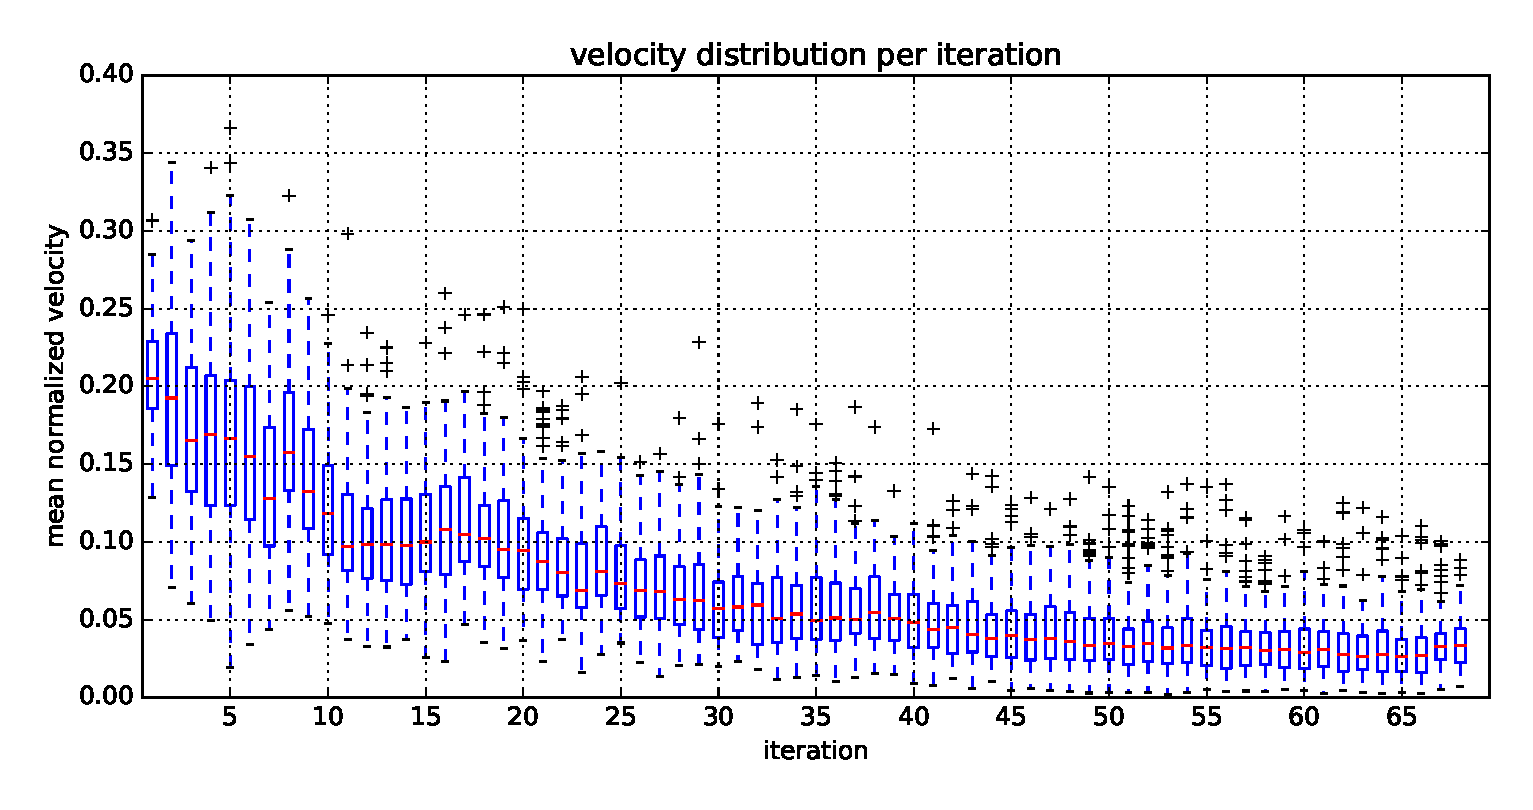
\includegraphics[width=\columnwidth]{evaluation/stator_vel.eps}
	\caption{Mean absolute velocity of the swarm's particles (from experiment 2)}
	\label{fig:stator_vel}
\end{figure}
\begin{figure}[!hbt]
	\centering
	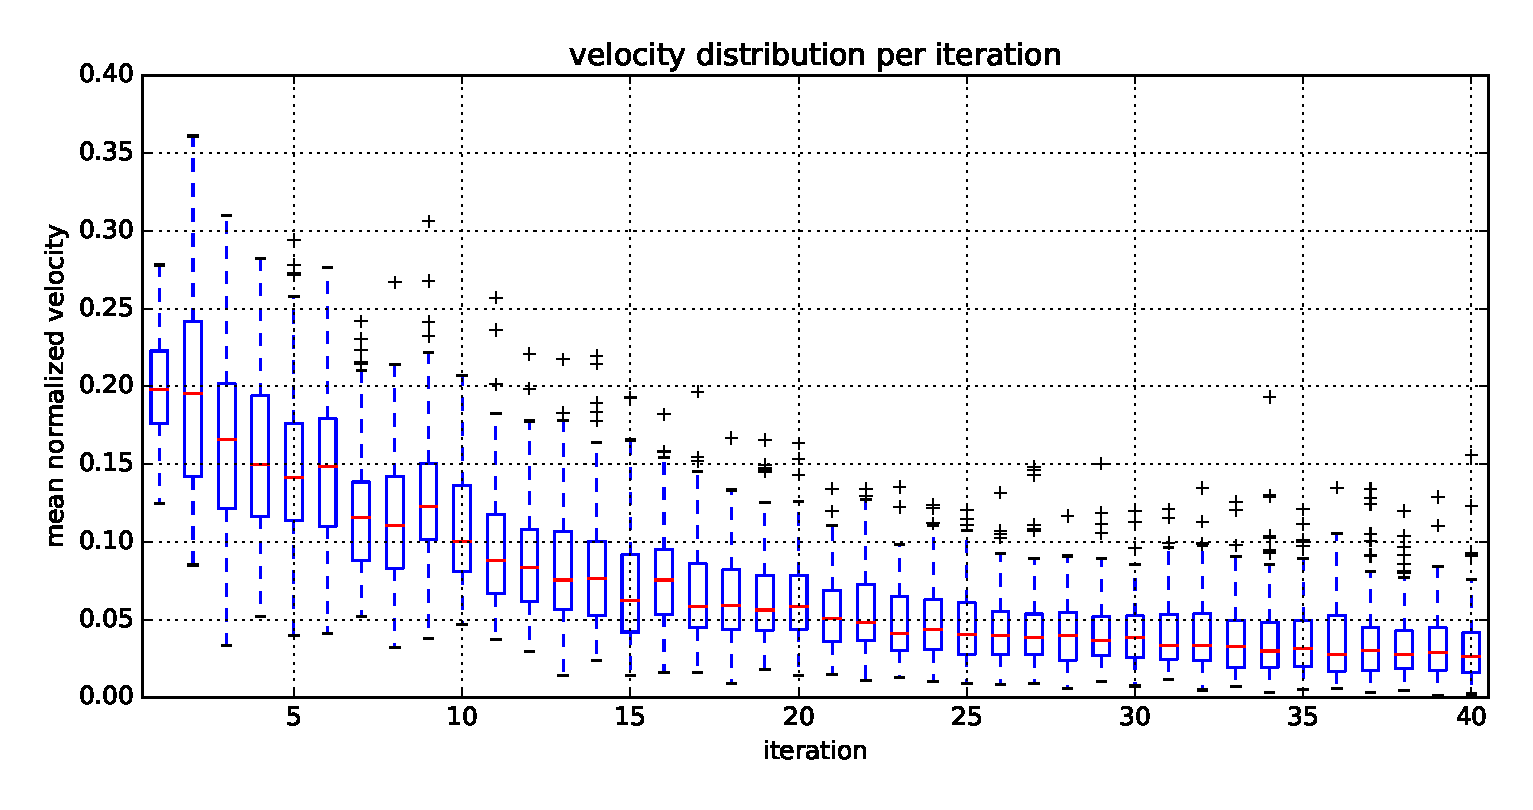
\includegraphics[width=\columnwidth]{evaluation/pm_vel.eps}
	\caption{Mean absolute velocity of the swarm's particles (from experiment 3)}
	\label{fig:pm_vel}
\end{figure}
\begin{figure}[!hbt]
	\centering
	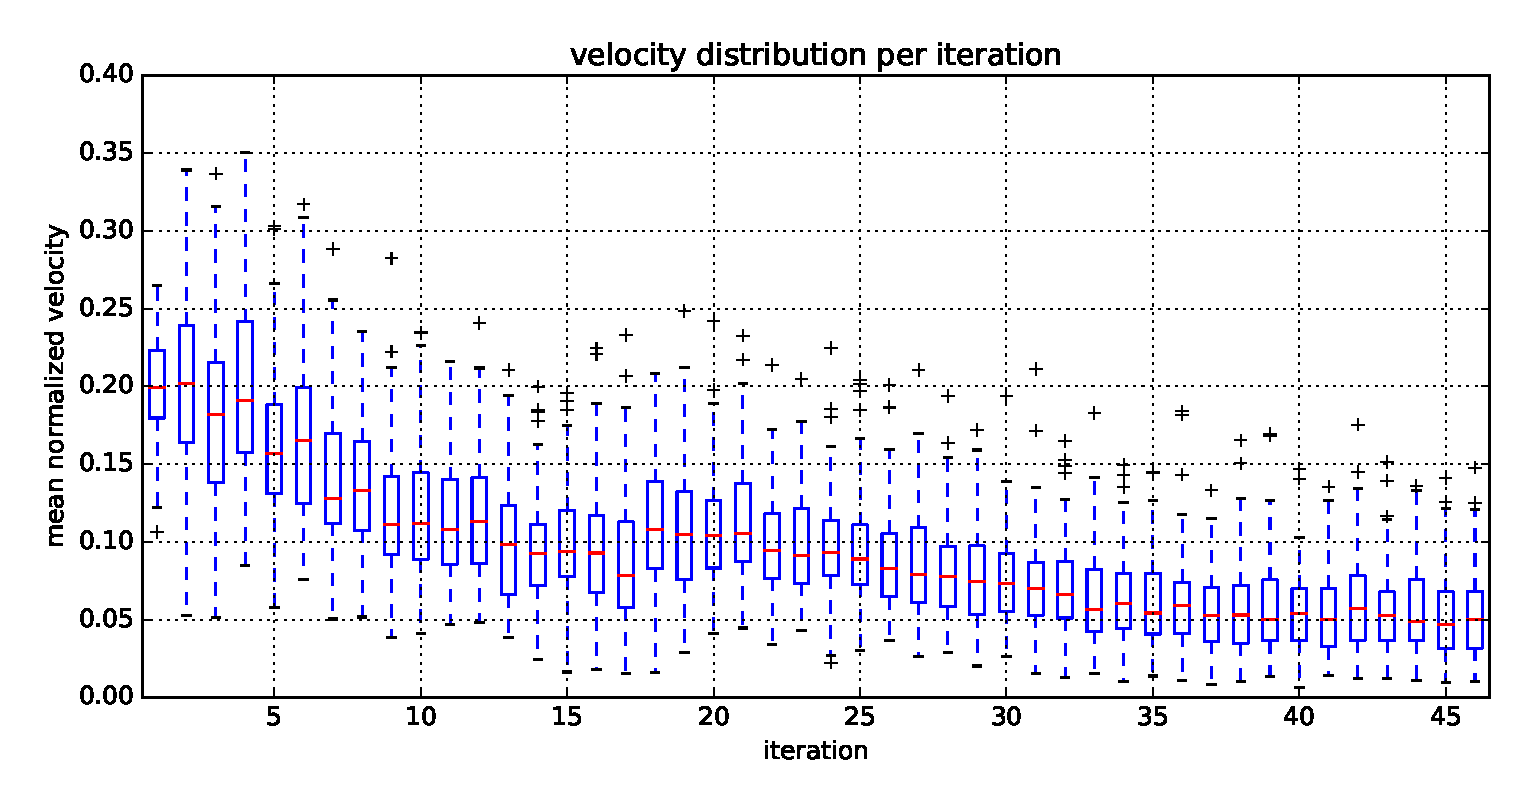
\includegraphics[width=\columnwidth]{evaluation/yoke_vel.eps}
	\caption{Mean absolute velocity of the swarm's particles (from experiment 4)}
	\label{fig:yoke_vel}
\end{figure}
\begin{figure}[!hbt]
	\centering
	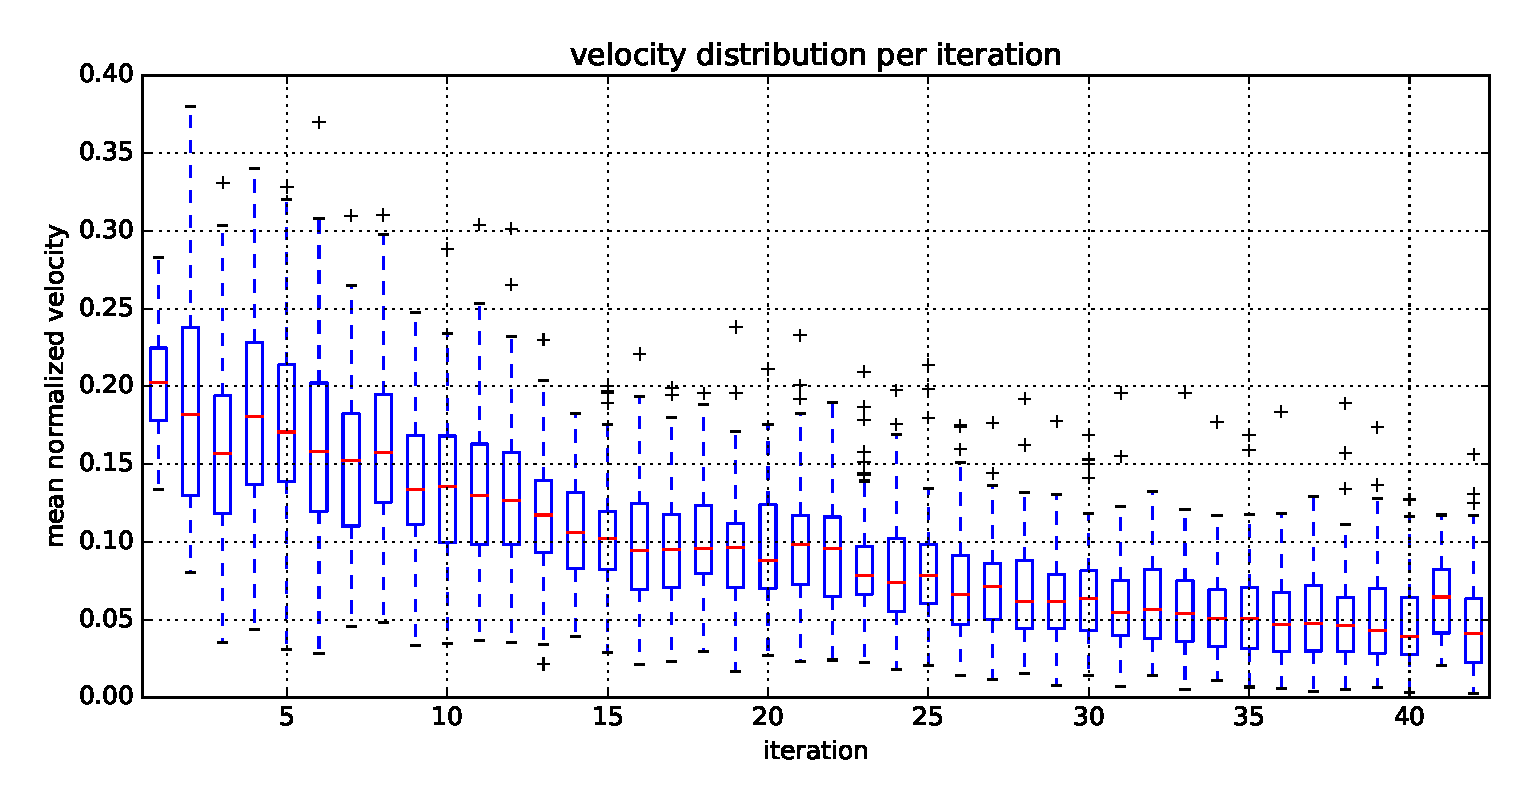
\includegraphics[width=\columnwidth]{evaluation/teeth_vel.eps}
	\caption{Mean absolute velocity of the swarm's particles (from experiment 5)}
	\label{fig:teeth_vel}
\end{figure}
\begin{figure}[!hbt]
	\centering
	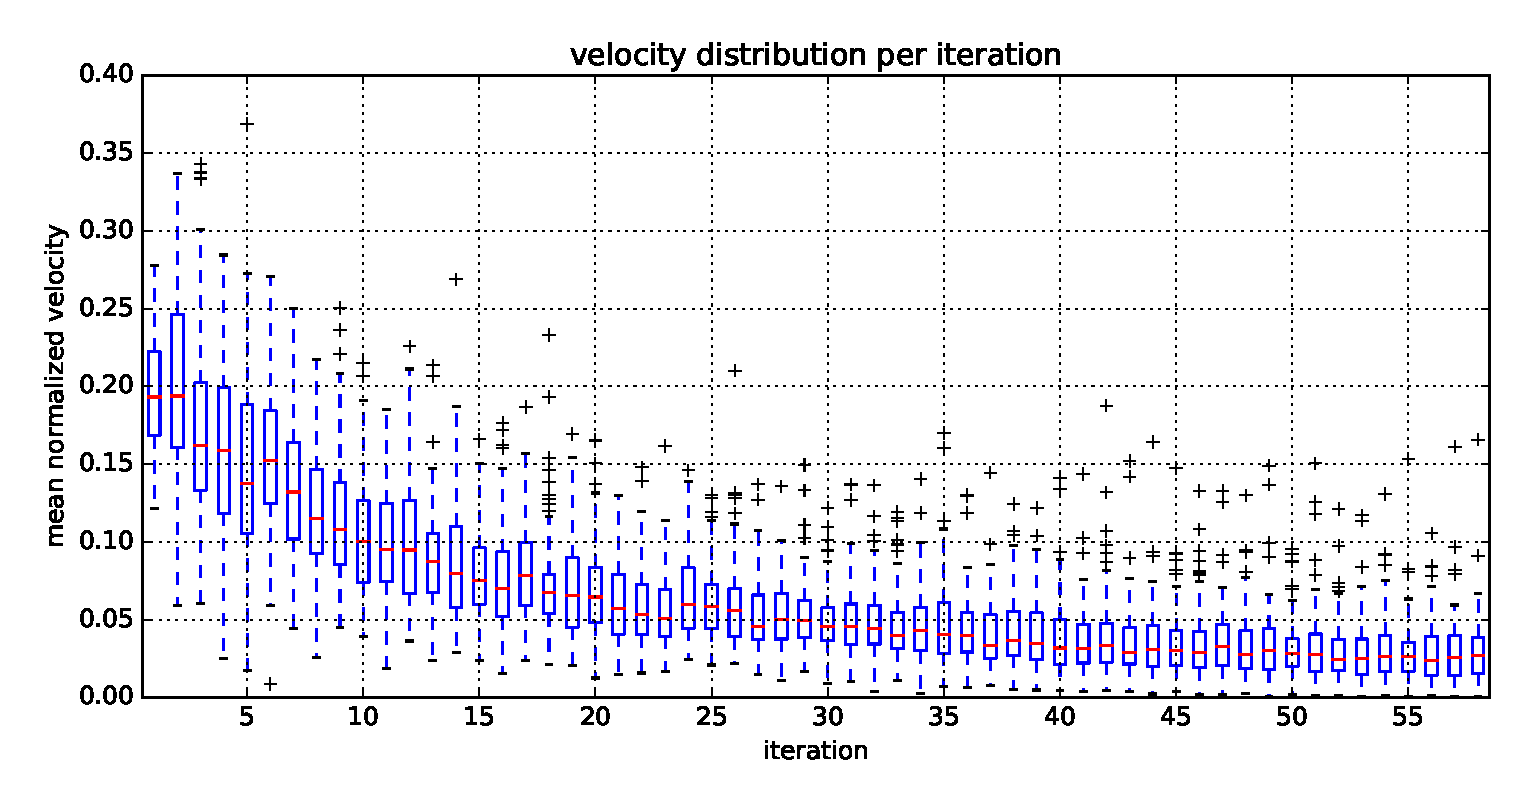
\includegraphics[width=\columnwidth]{evaluation/winding_vel.eps}
	\caption{Mean absolute velocity of the swarm's particles (from experiment 6)}
	\label{fig:winding_vel}
\end{figure}\clearpage

\section{Swarm Evaluation Trends}
\label{app:evaluation}
Evaluation plots encompass fig. \ref{fig:stator_eval}, \ref{fig:pm_eval}, \ref{fig:yoke_eval}, \ref{fig:teeth_eval} and \ref{fig:winding_eval}.
\begin{figure}[!hbt]
	\centering
	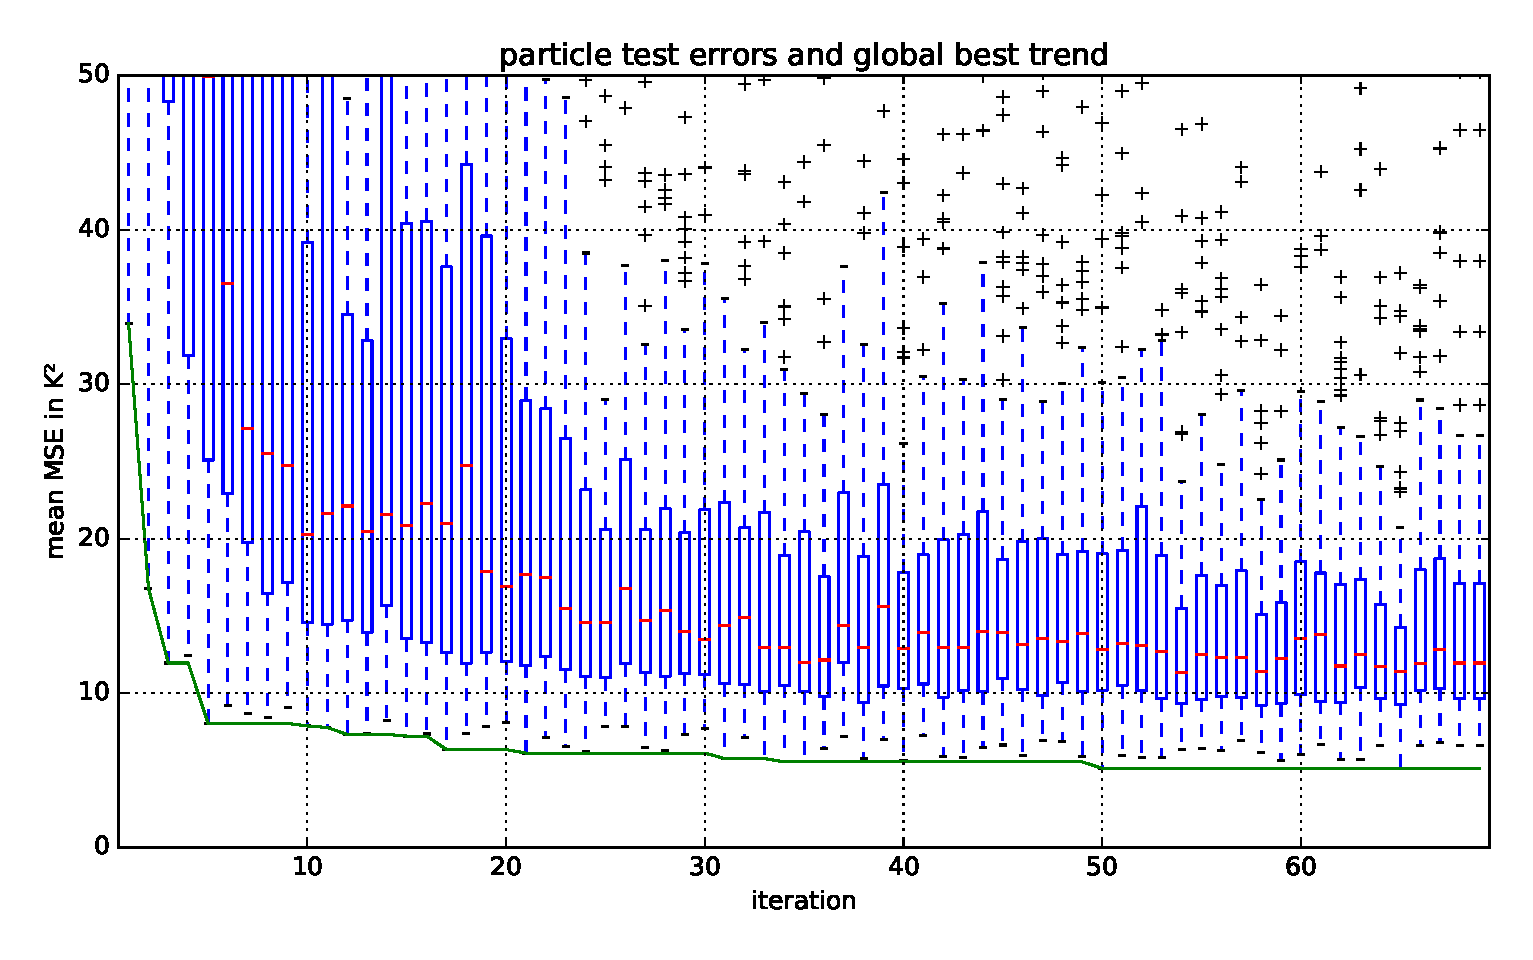
\includegraphics[width=\columnwidth]{evaluation/stator_eval.eps}
	\caption{Particle test scores over all iterations as box plots and the found best site's score as green line (from experiment 2)}
	\label{fig:stator_eval}
\end{figure}
\begin{figure}[!hbt]
	\centering
	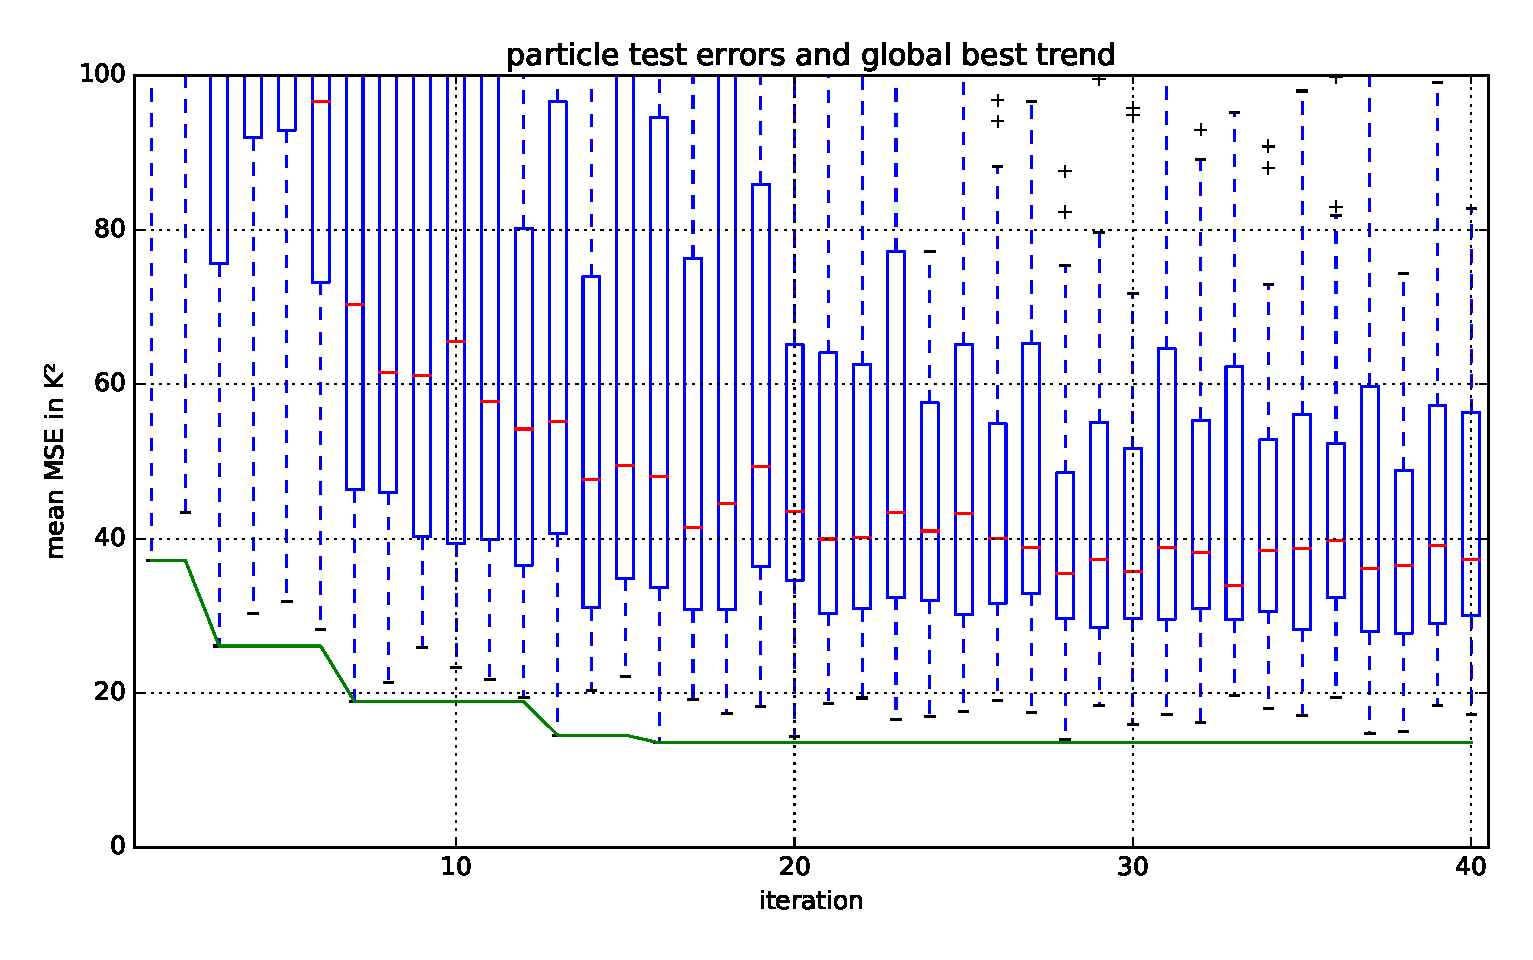
\includegraphics[width=\columnwidth]{evaluation/pm_eval.eps}
	\caption{Particle test scores over all iterations as box plots and the found best site's score as green line (from experiment 3)}
	\label{fig:pm_eval}
\end{figure}
\begin{figure}[!hbt]
	\centering
	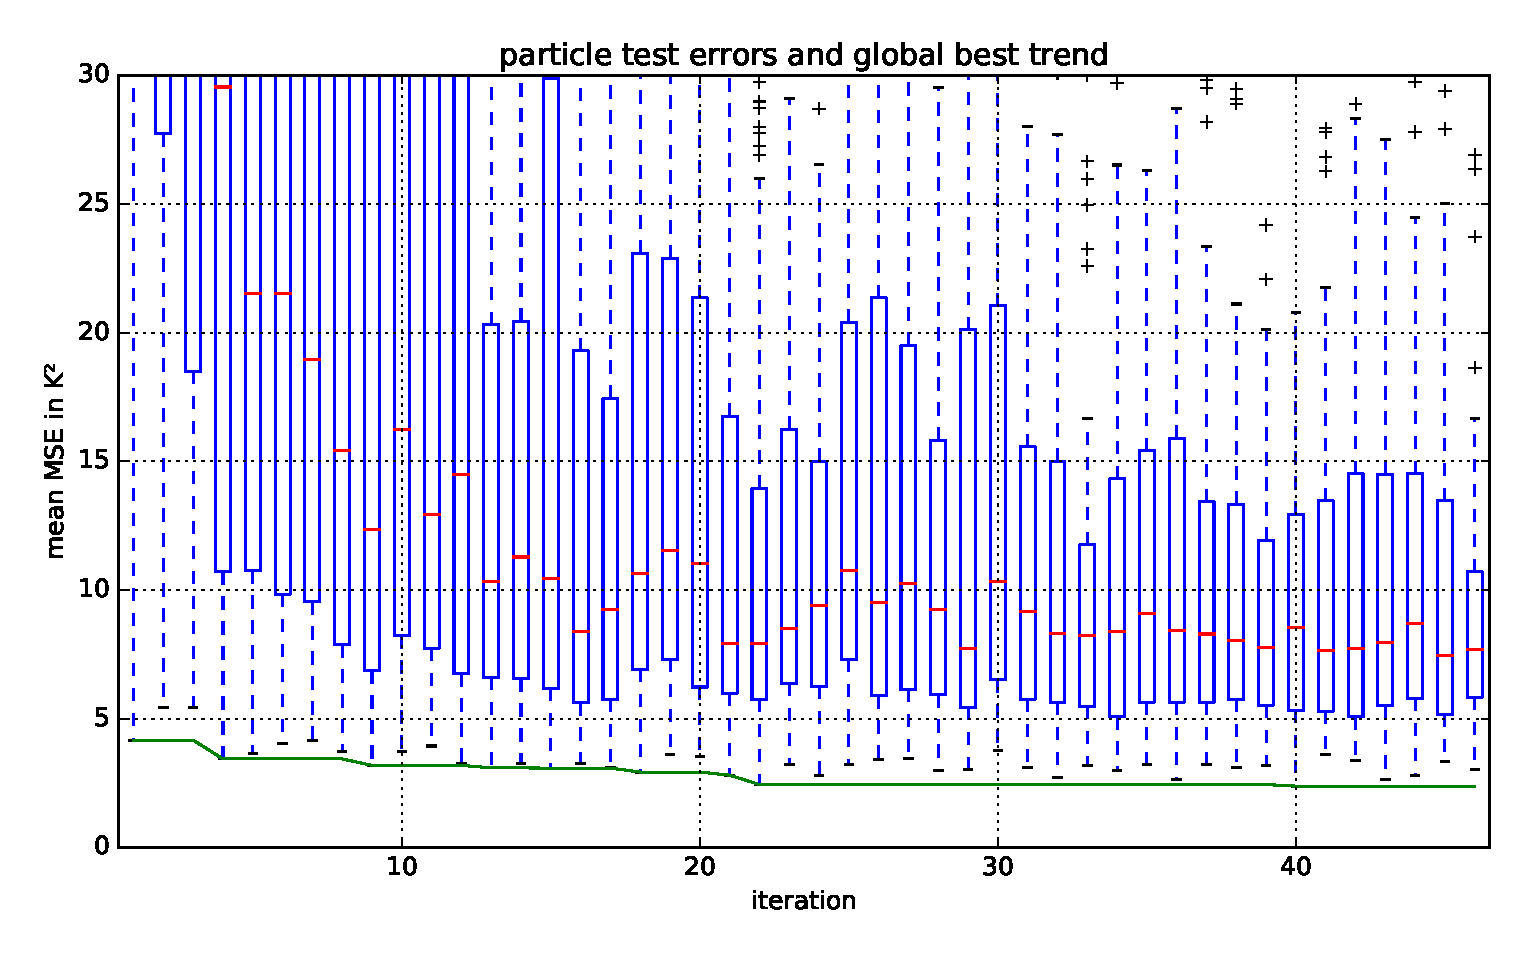
\includegraphics[width=\columnwidth]{evaluation/yoke_eval.eps}
	\caption{Particle test scores over all iterations as box plots and the found best site's score as green line (from experiment 4)}
	\label{fig:yoke_eval}
\end{figure}
\begin{figure}[!hbt]
	\centering
	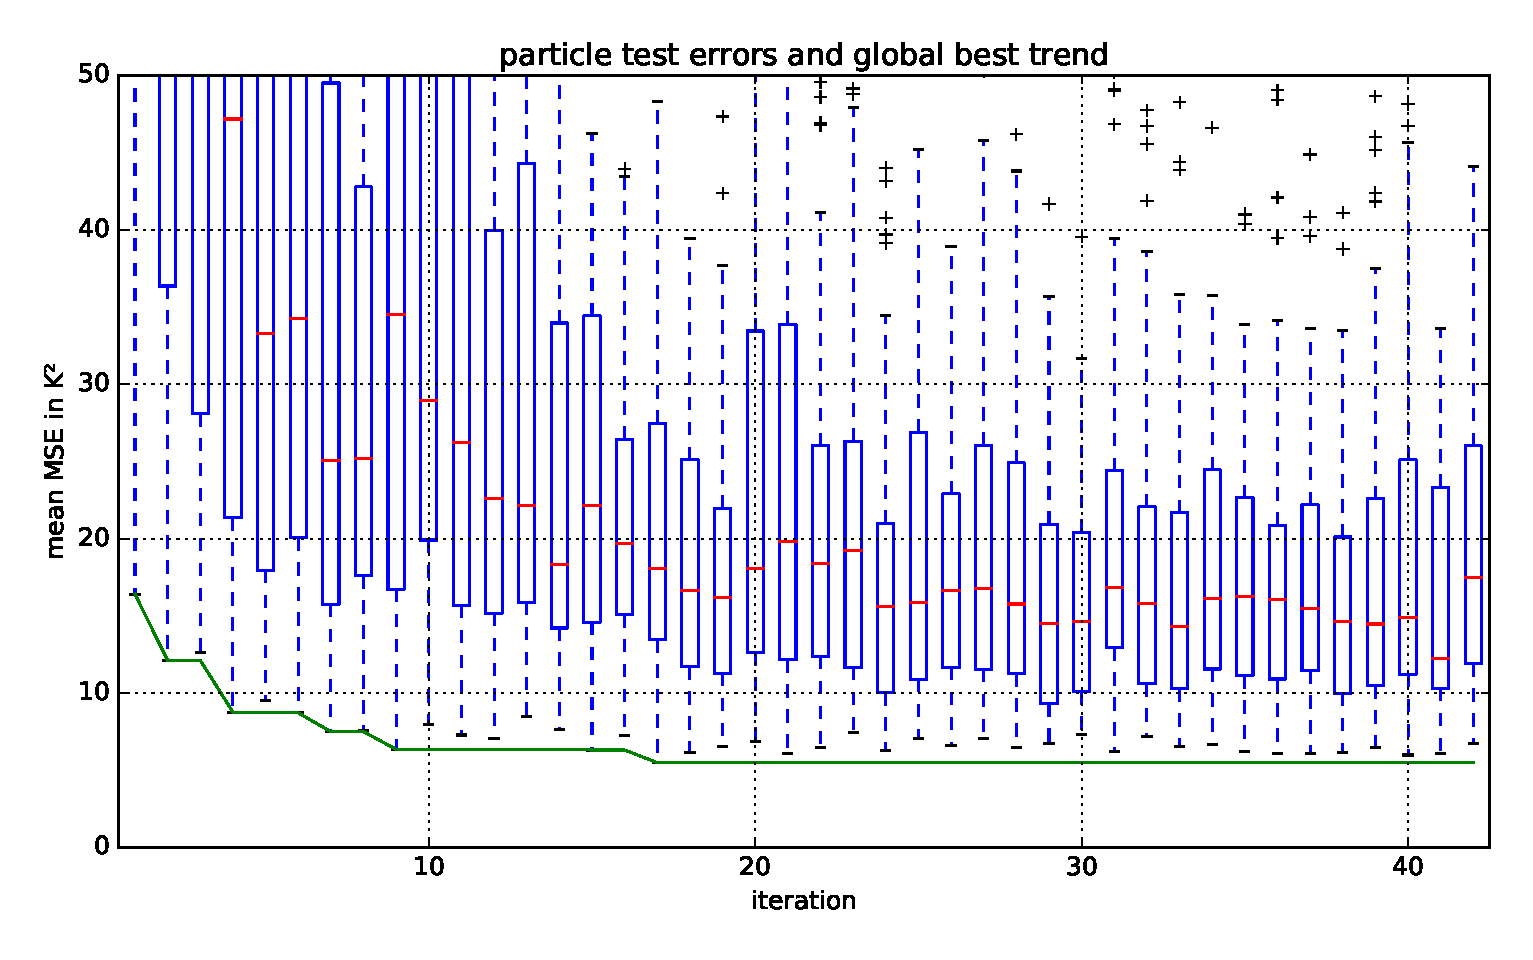
\includegraphics[width=\columnwidth]{evaluation/teeth_eval.eps}
	\caption{Particle test scores over all iterations as box plots and the found best site's score as green line (from experiment 5)}
	\label{fig:teeth_eval}
\end{figure}
\begin{figure}[!hbt]
	\centering
	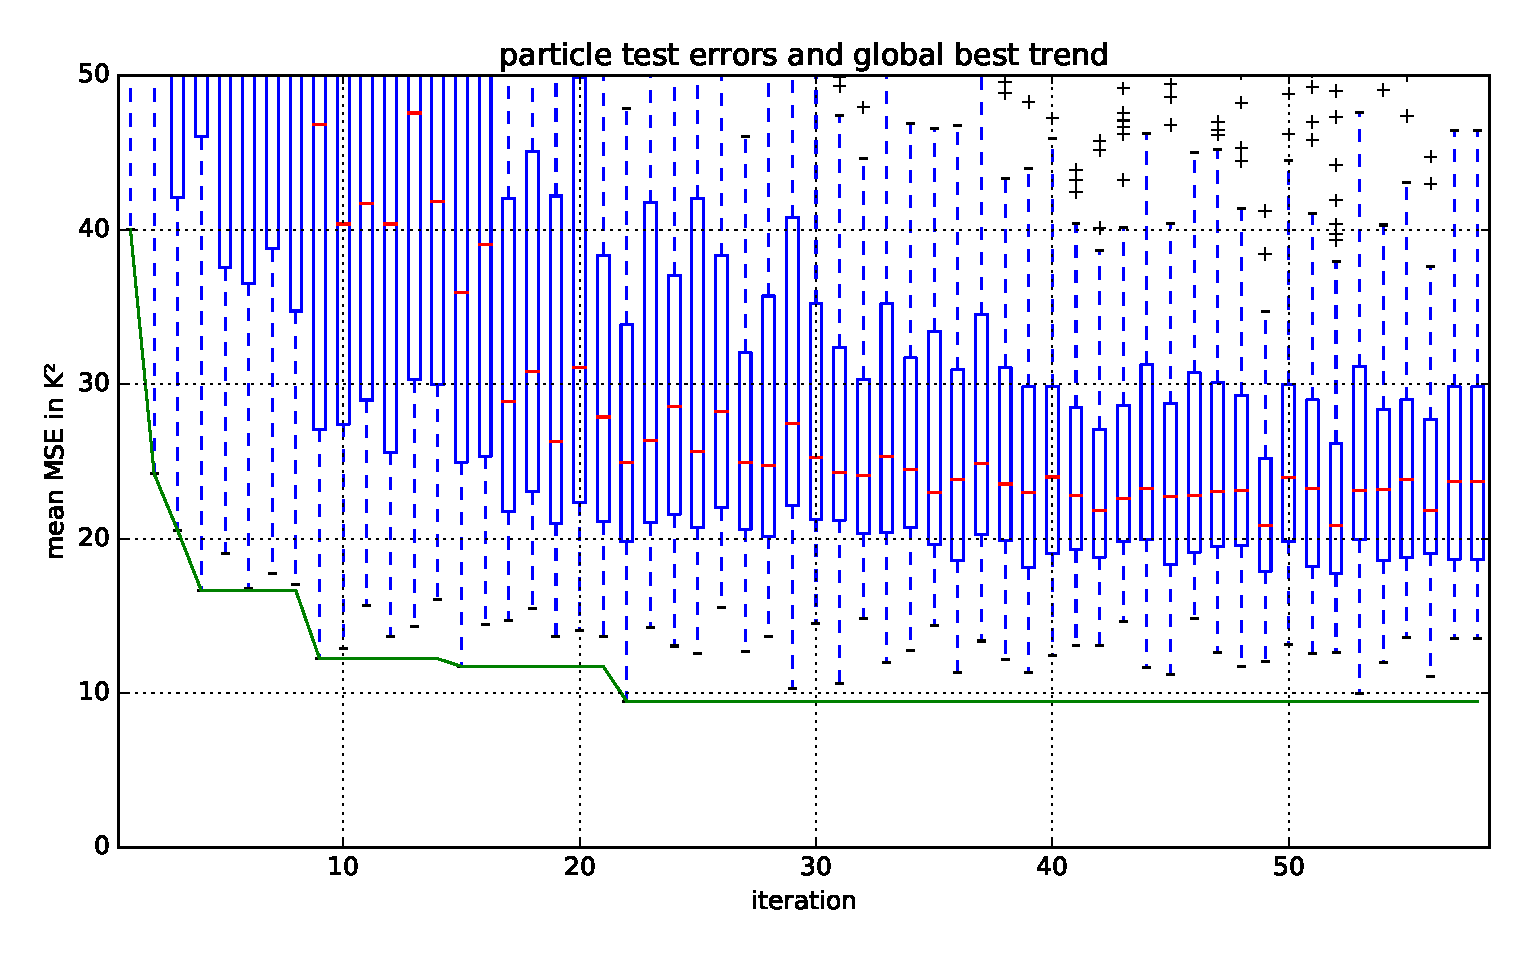
\includegraphics[width=\columnwidth]{evaluation/winding_eval.eps}
	\caption{Particle test scores over all iterations as box plots and the found best site's score as green line (from experiment 6)}
	\label{fig:winding_eval}
\end{figure}\clearpage

\section{Parameter Distributions}
\label{app:param_dist}
Distribution plots encompass fig. \ref{fig:stator_param_dist}, \ref{fig:pm_param_dist}, \ref{fig:yoke_param_dist}, \ref{fig:teeth_param_dist} and \ref{fig:winding_param_dist}.
\begin{figure}[!hbt]
	\centering
	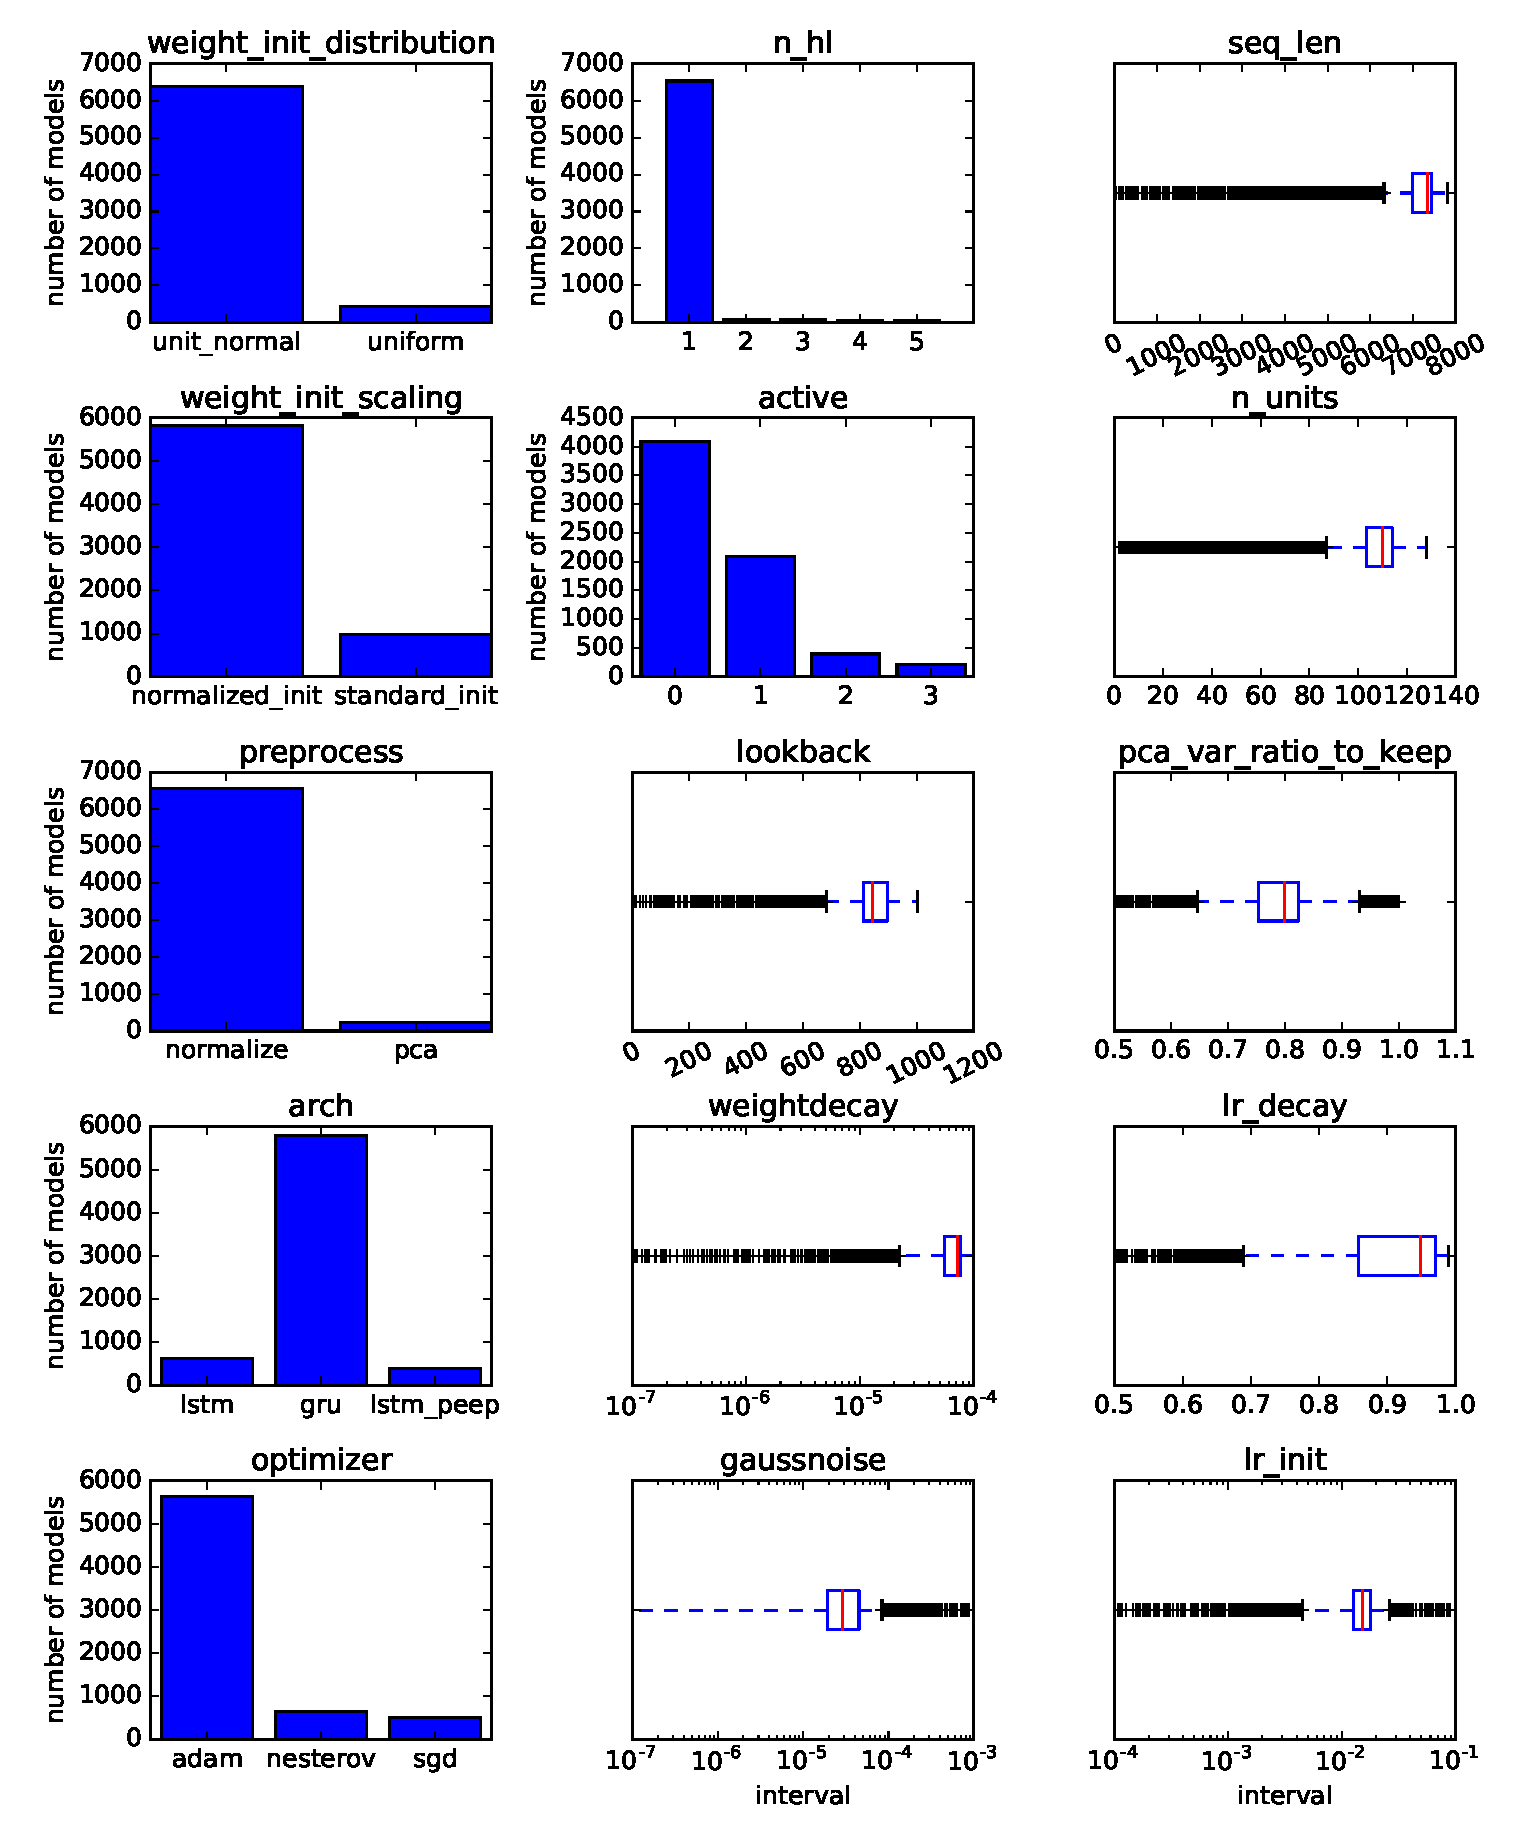
\includegraphics[width=\columnwidth]{evaluation/stator_paramdist.eps}
	\caption{Bar plots and box plots depicting the distribution of each hyper-parameter over all \gls{pso} iterations (from experiment 2)}
	\label{fig:stator_param_dist}
\end{figure}
\begin{figure}[!hbt]
	\centering
	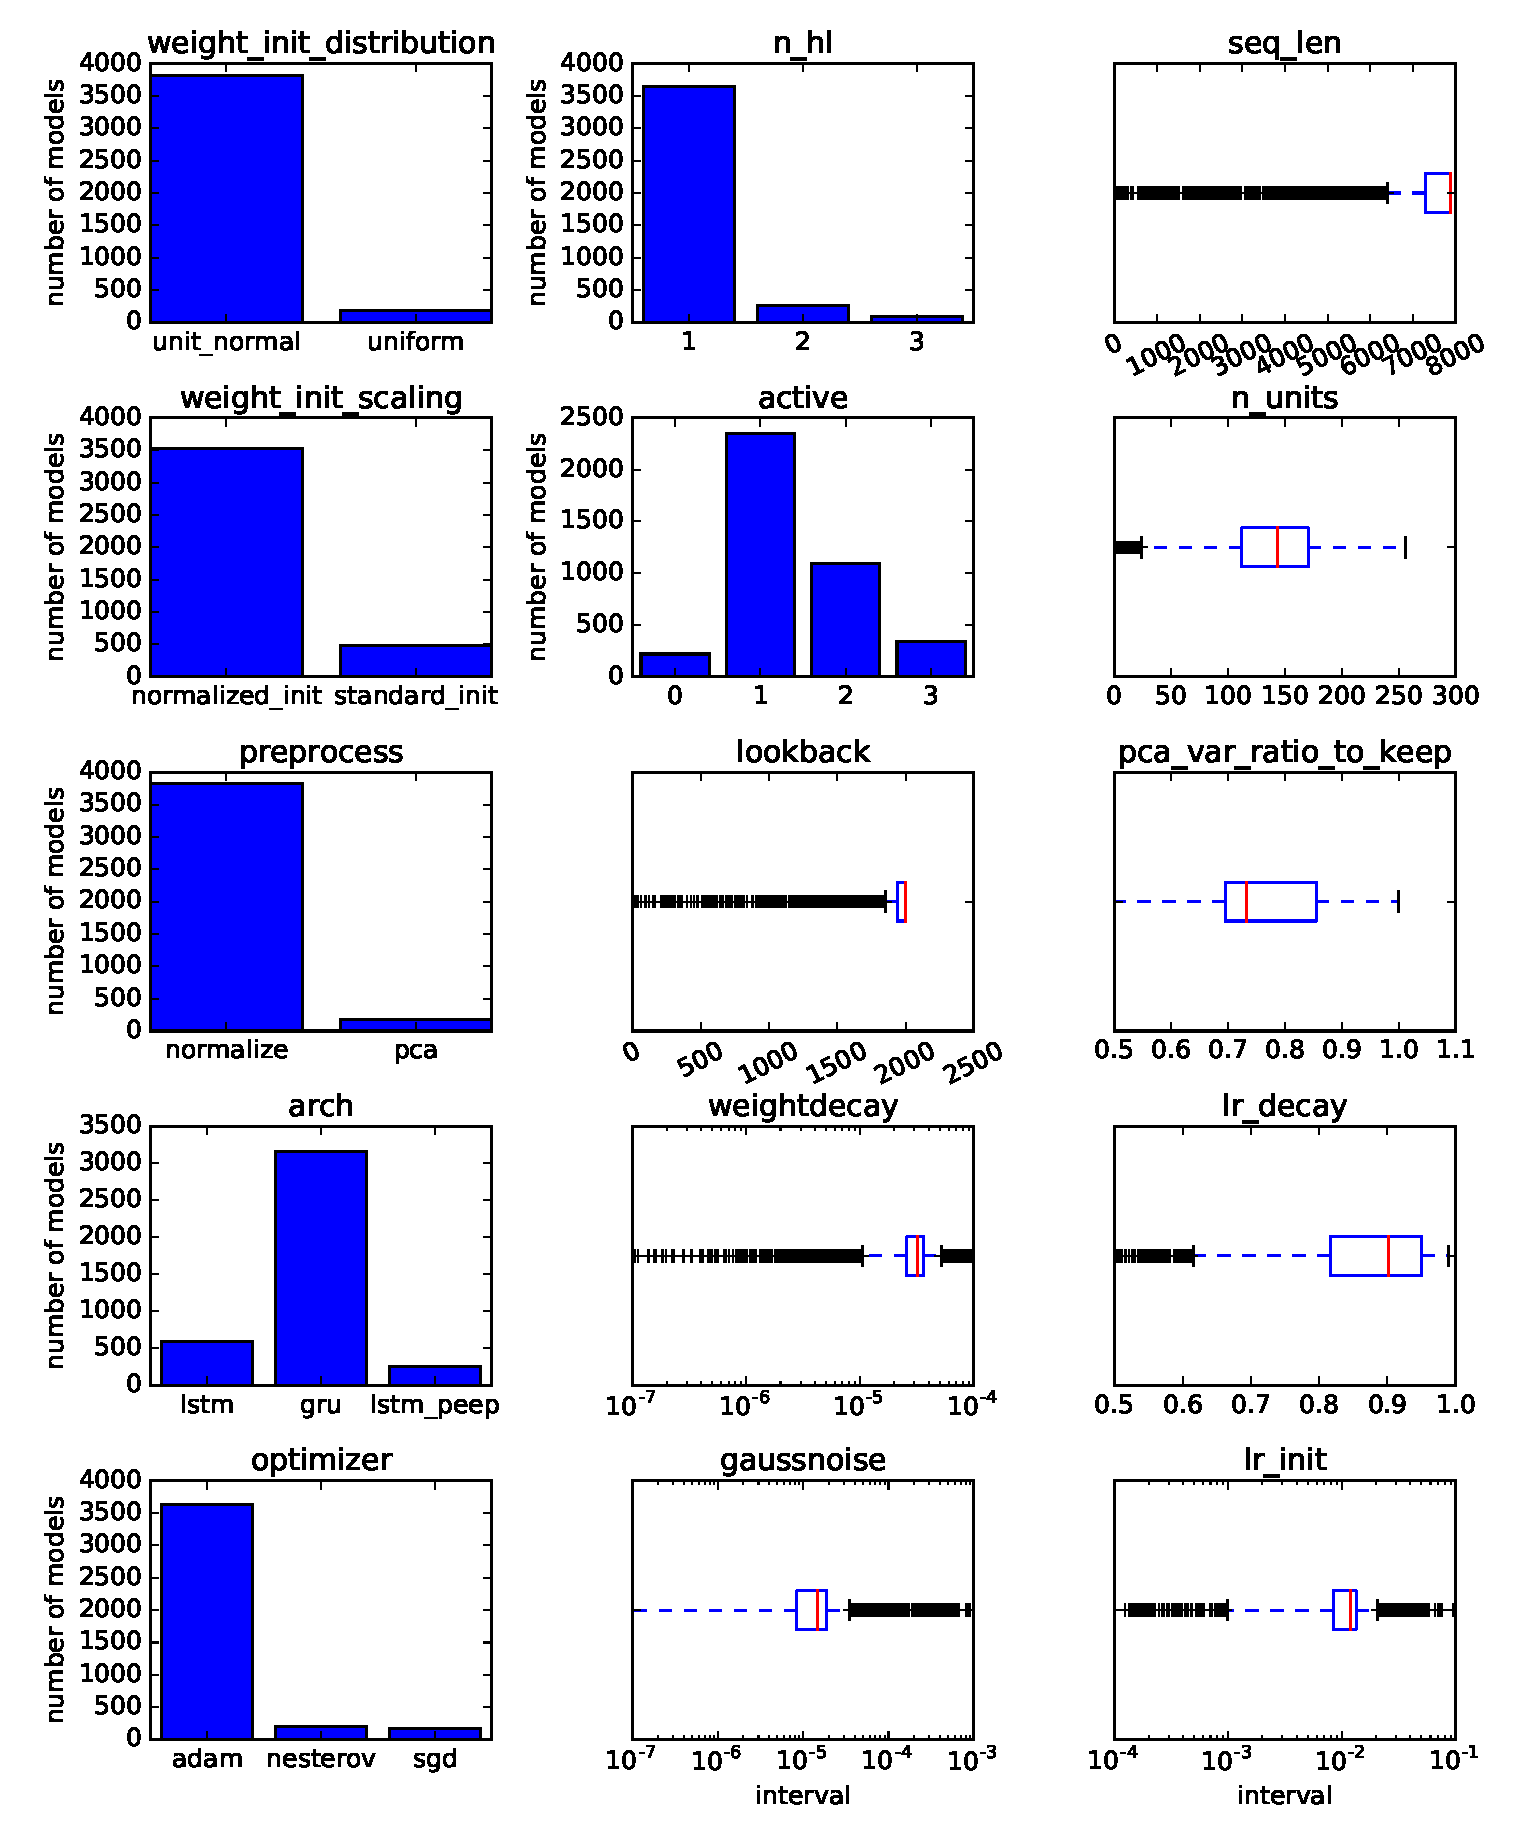
\includegraphics[width=\columnwidth]{evaluation/pm_paramdist.eps}
	\caption{Bar plots and box plots depicting the distribution of each hyper-parameter over all \gls{pso} iterations (from experiment 3)}
	\label{fig:pm_param_dist}
\end{figure}
\begin{figure}[!hbt]
	\centering
	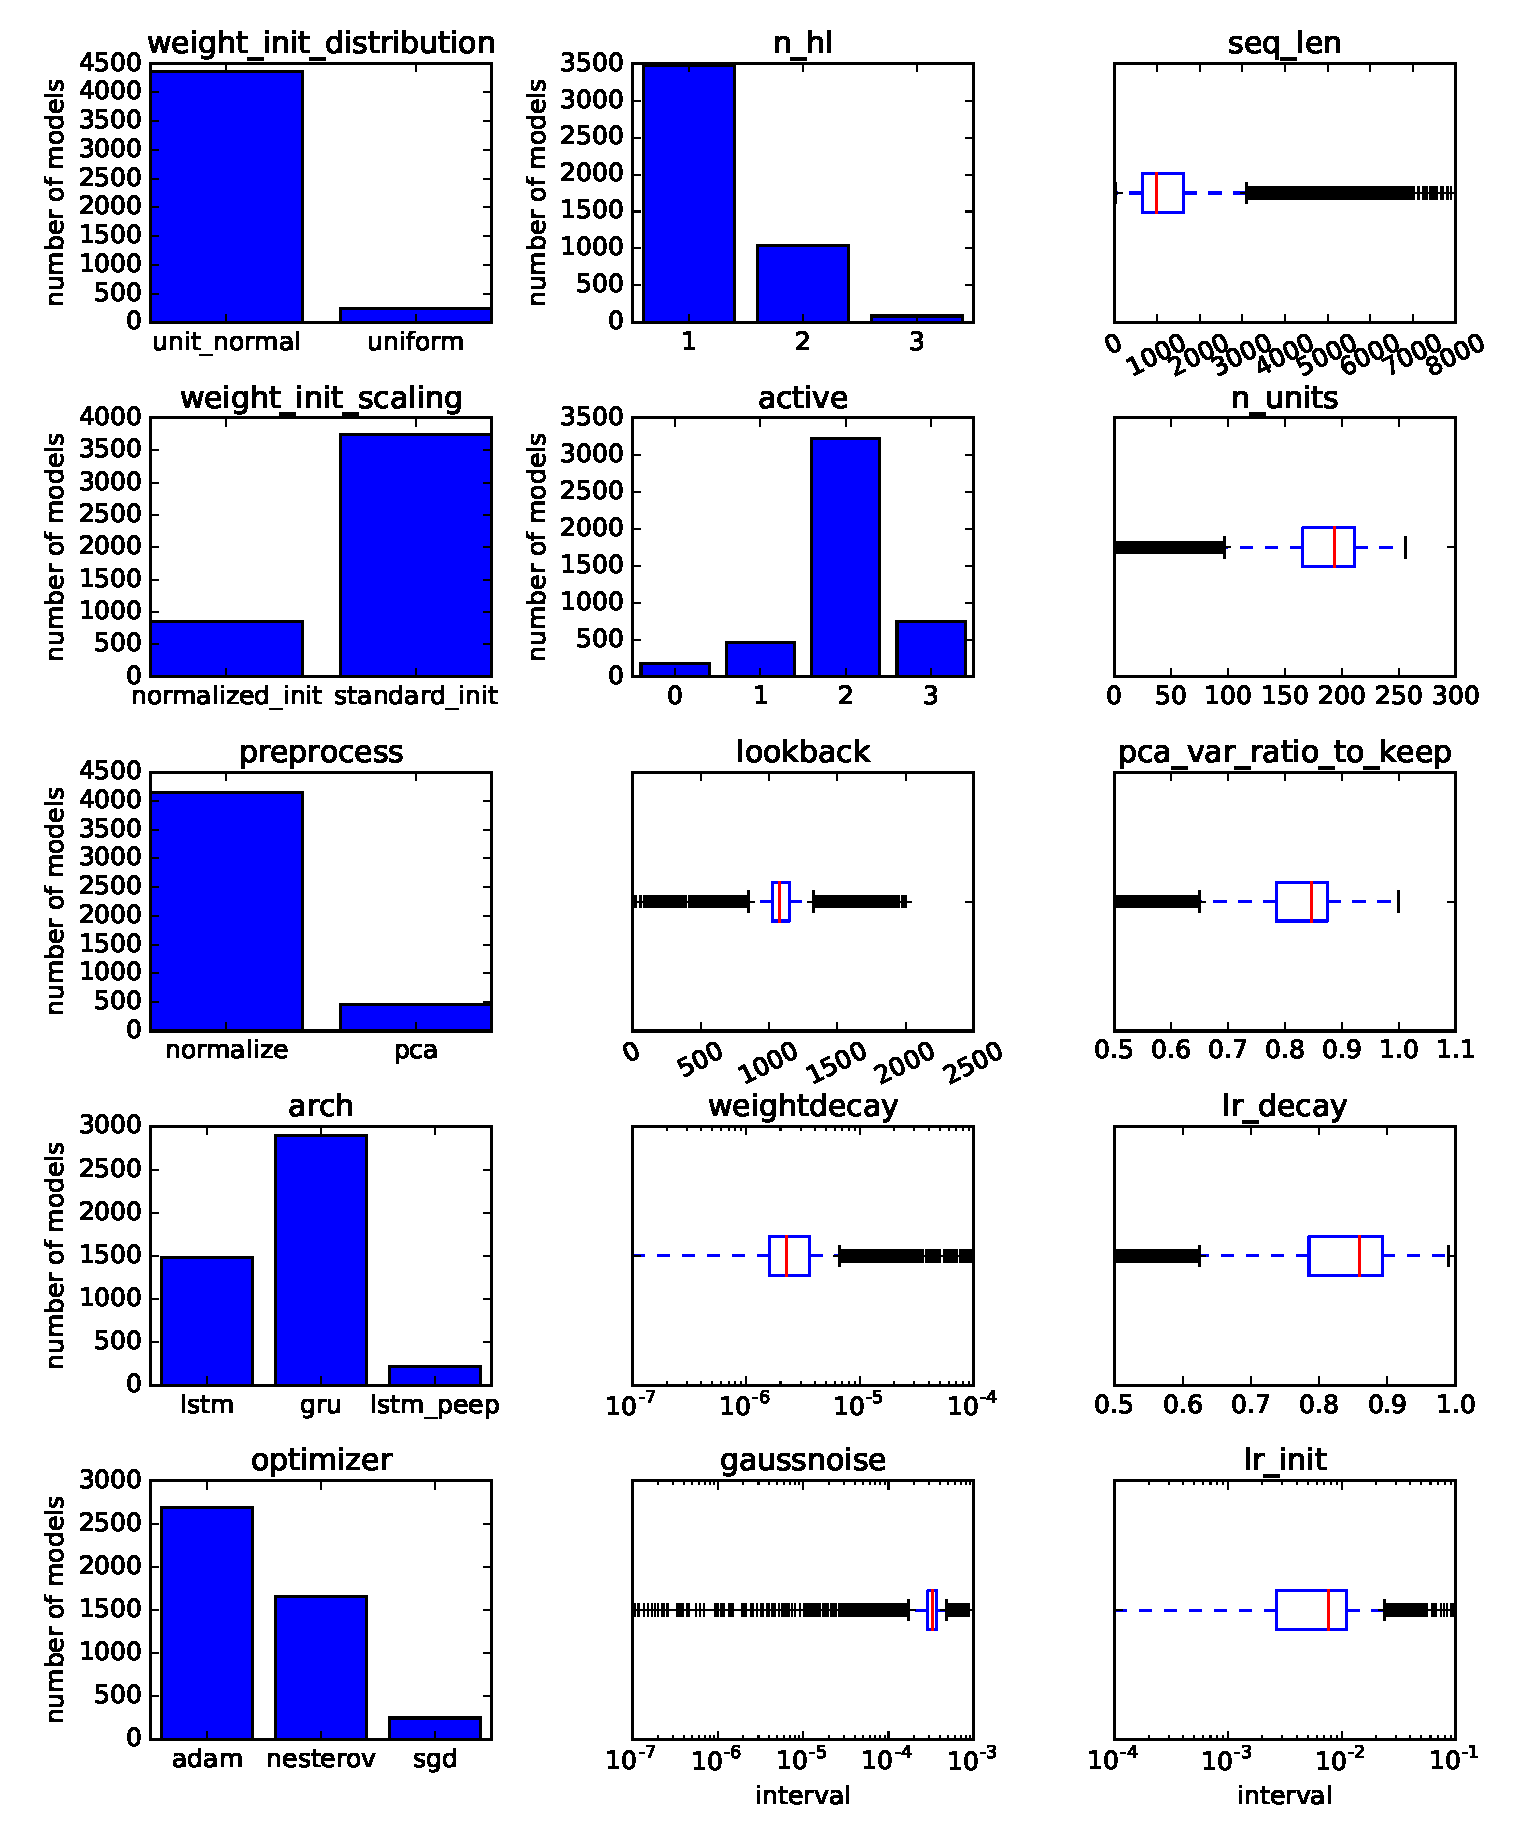
\includegraphics[width=\columnwidth]{evaluation/yoke_paramdist.eps}
	\caption{Bar plots and box plots depicting the distribution of each hyper-parameter over all \gls{pso} iterations (from experiment 4)}
	\label{fig:yoke_param_dist}
\end{figure}
\begin{figure}[!hbt]
	\centering
	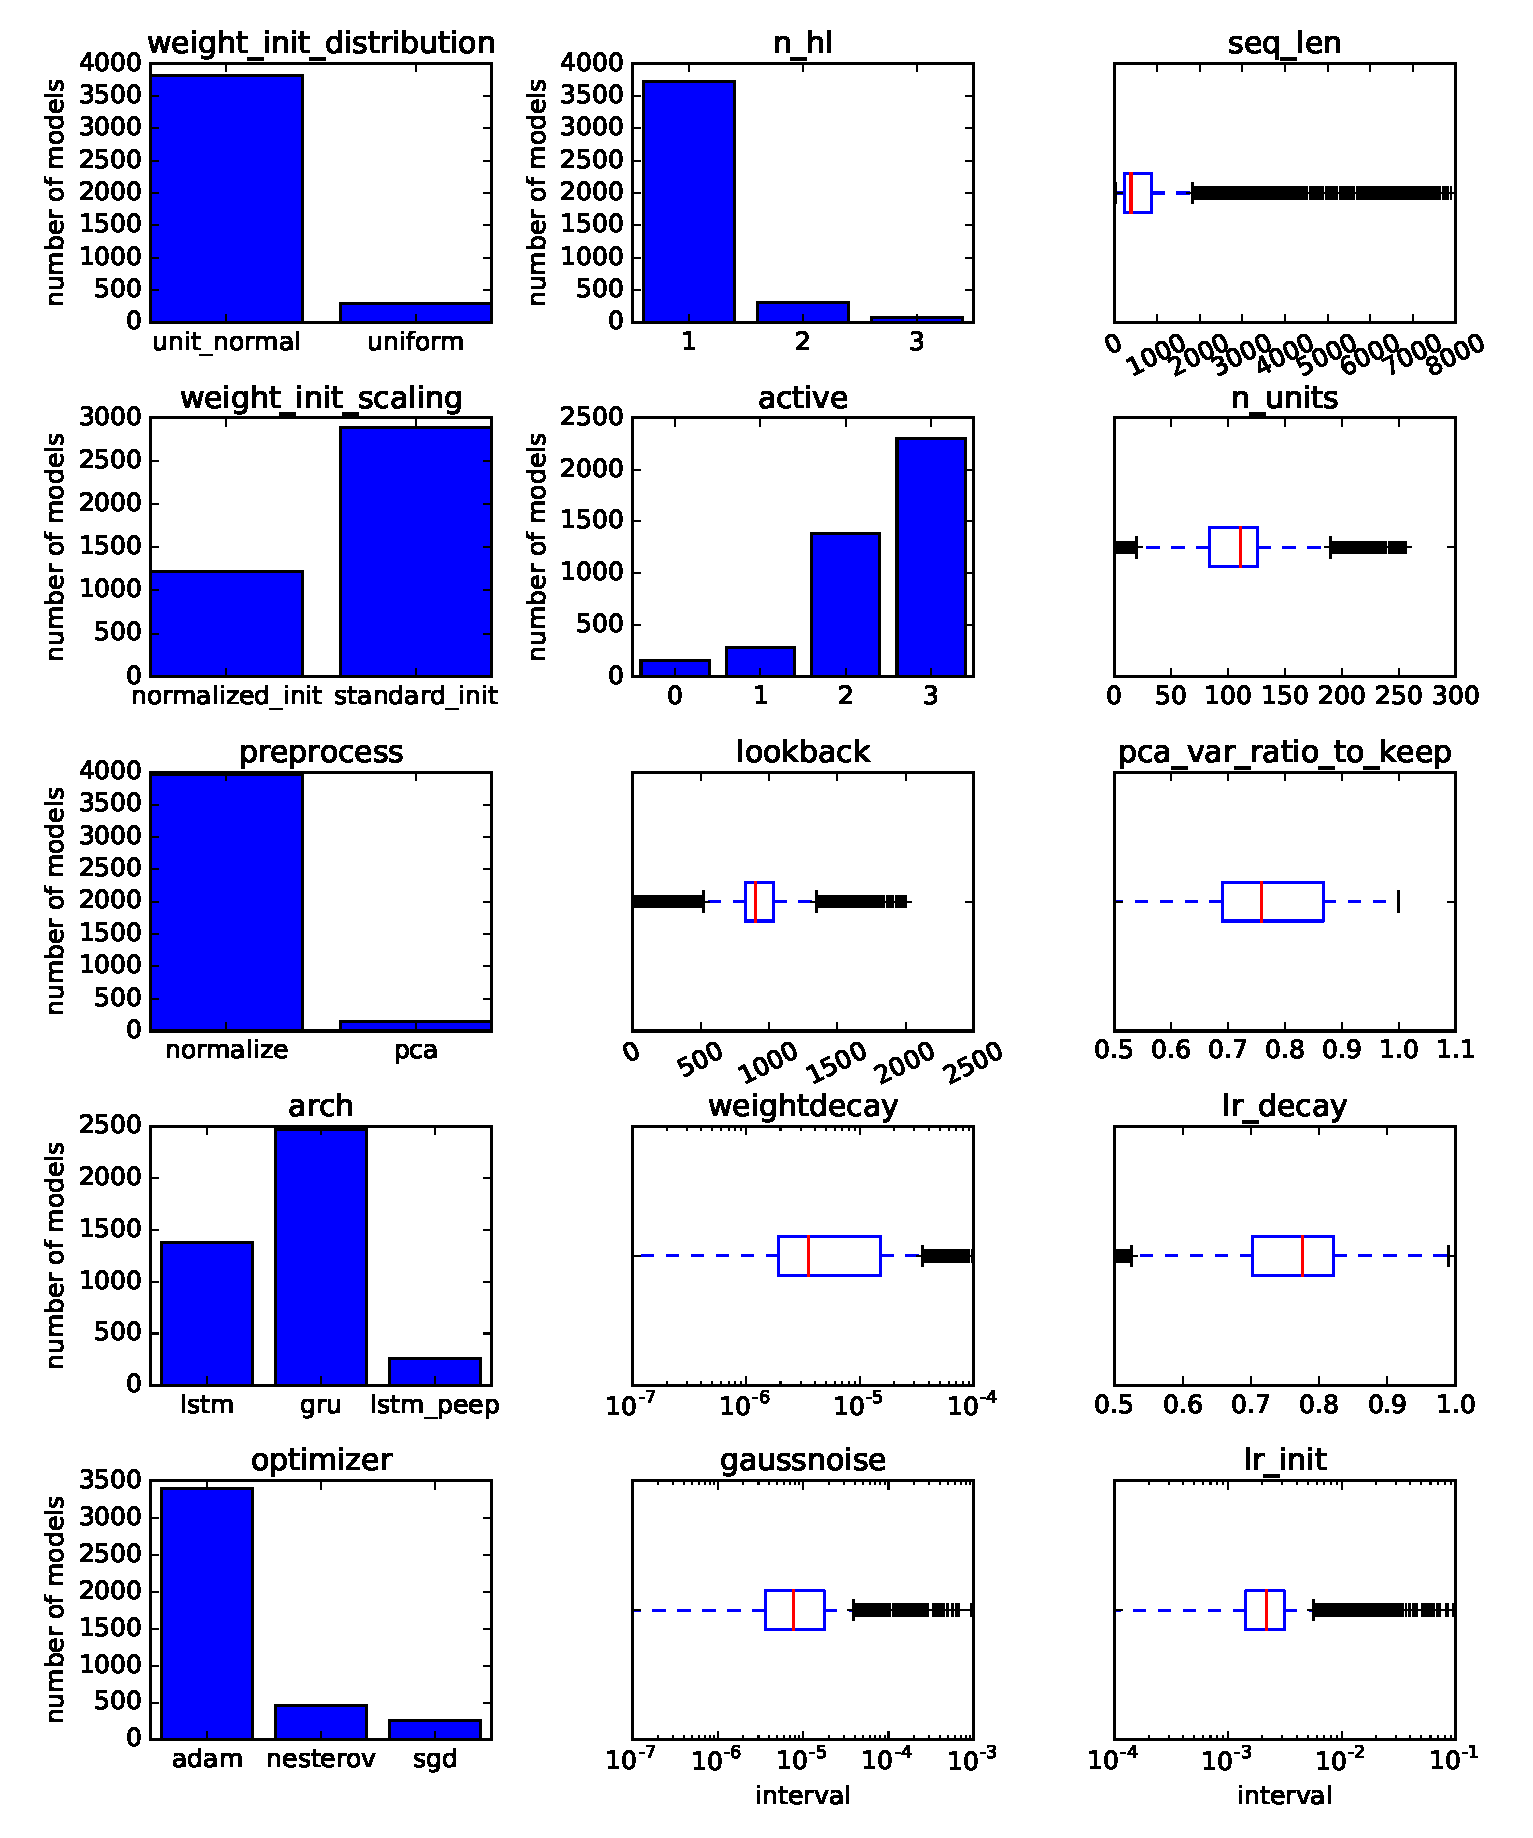
\includegraphics[width=\columnwidth]{evaluation/teeth_paramdist.eps}
	\caption{Bar plots and box plots depicting the distribution of each hyper-parameter over all \gls{pso} iterations (from experiment 5)}
	\label{fig:teeth_param_dist}
\end{figure}
\begin{figure}[!hbt]
	\centering
	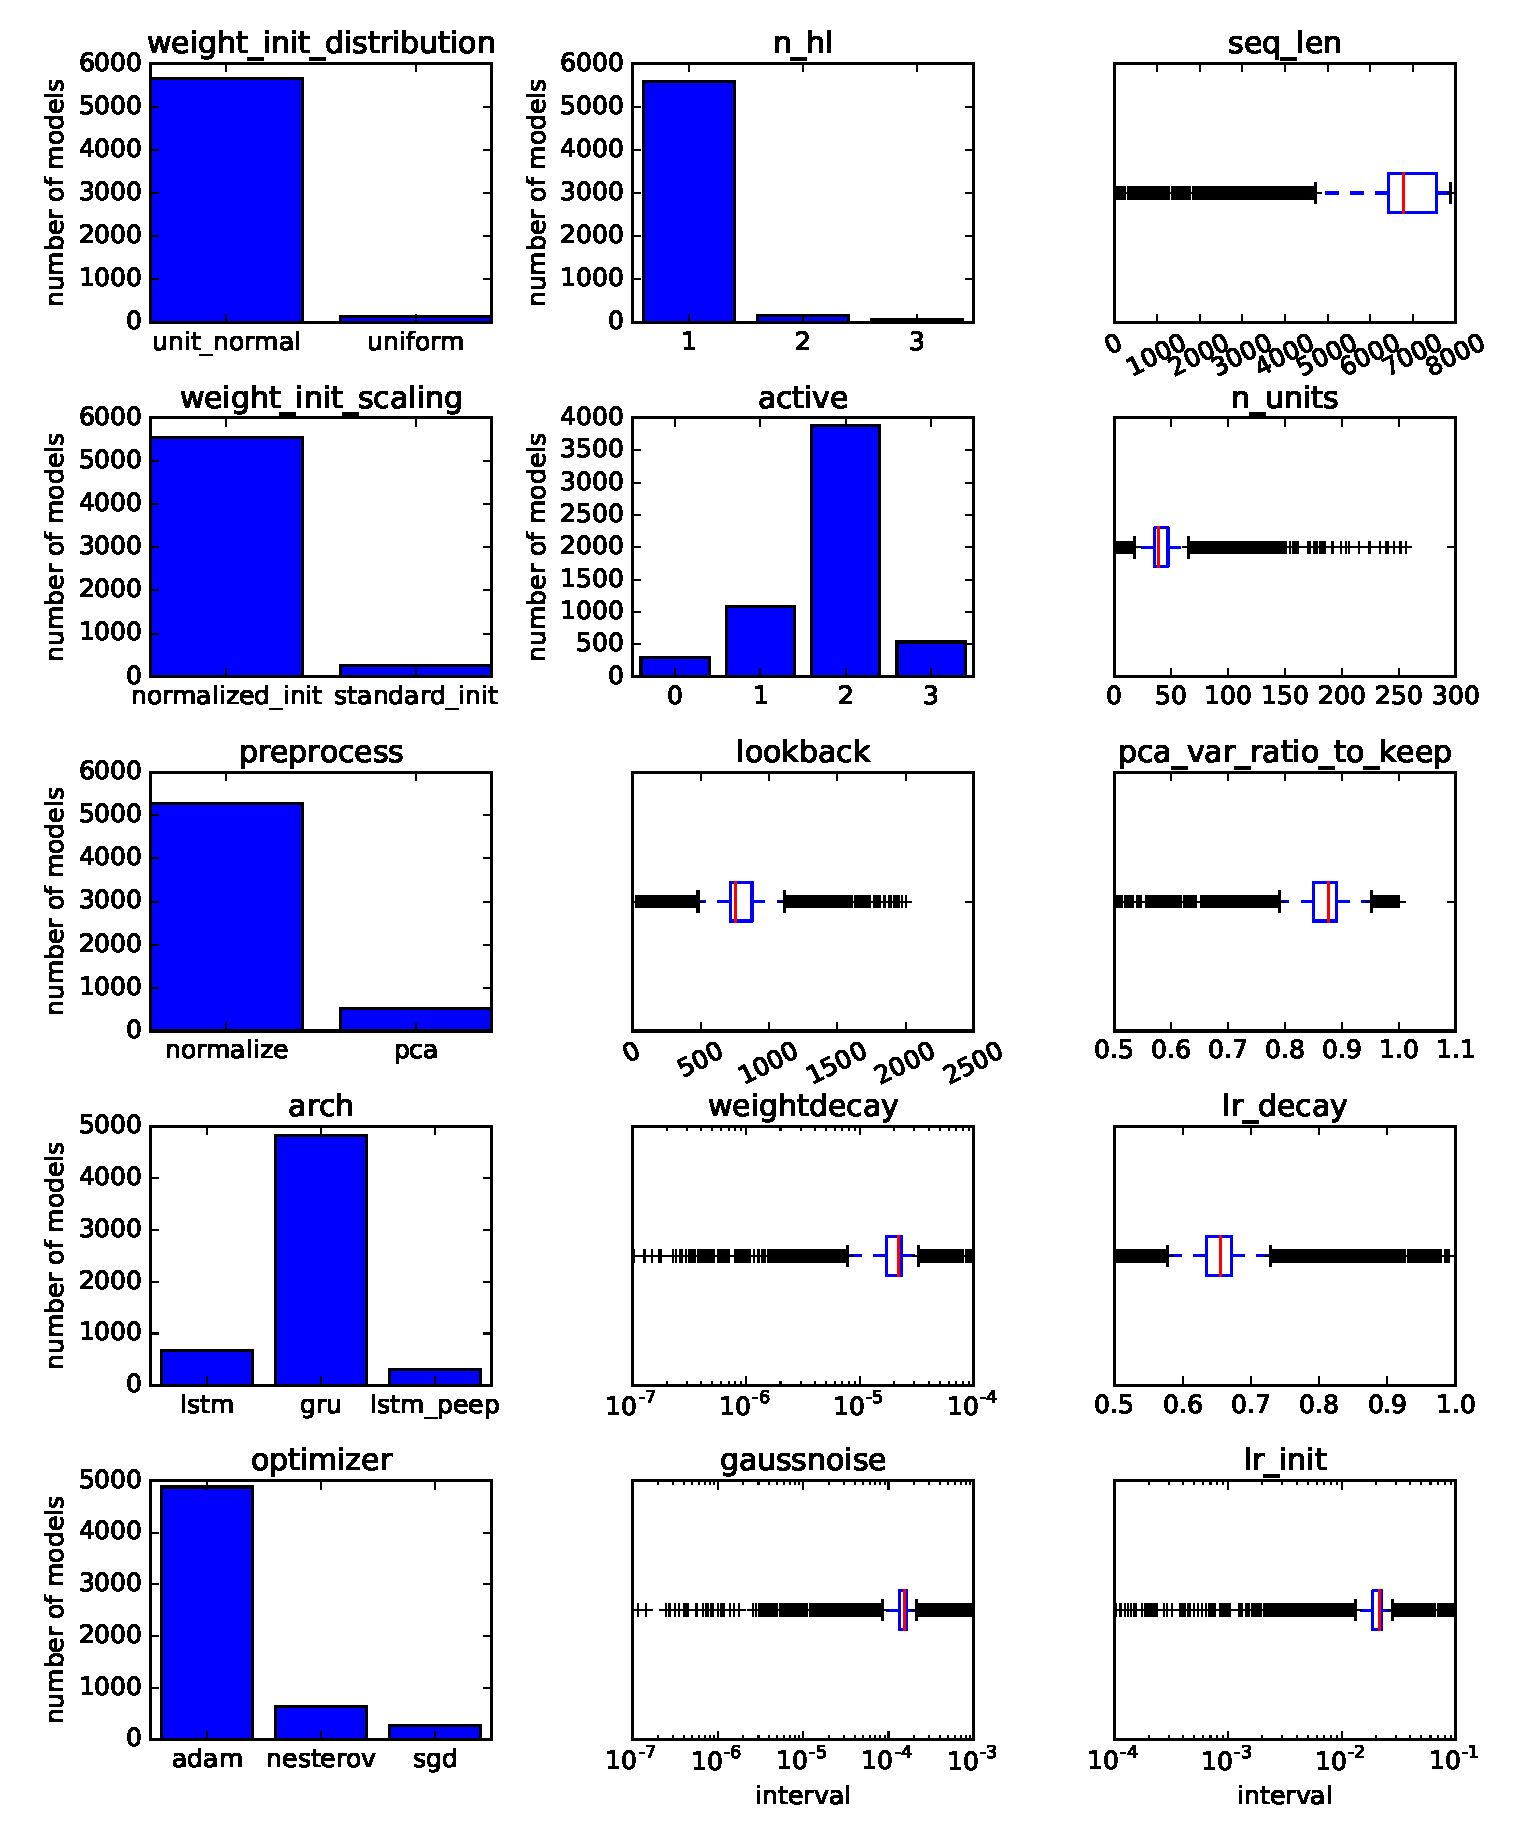
\includegraphics[width=\columnwidth]{evaluation/winding_paramdist.eps}
	\caption{Bar plots and box plots depicting the distribution of each hyper-parameter over all \gls{pso} iterations (from experiment 6)}
	\label{fig:winding_param_dist}
\end{figure}\clearpage

\section{Parameter Variance Trends}
\label{app:param_var}

Parameter variance trends encompass fig. \ref{fig:stator_var}, \ref{fig:pm_var}, \ref{fig:yoke_var}, \ref{fig:teeth_var} and \ref{fig:winding_var}.
\begin{figure}[!hbt]
	\centering
	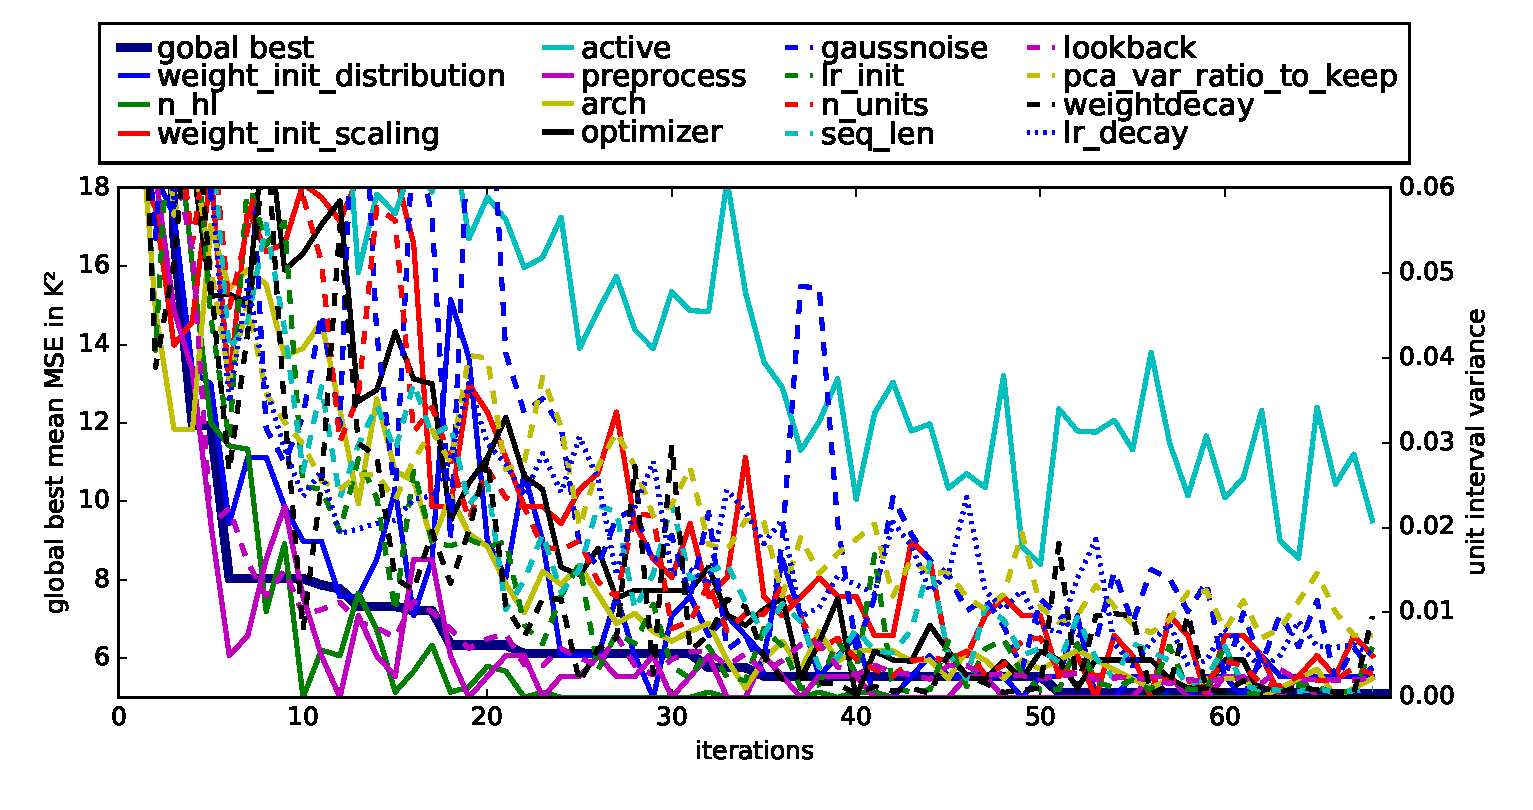
\includegraphics[width=\textwidth]{evaluation/stator_var.eps}
	\caption{Hyper-parameter variance over \gls{pso} iterations (from experiment 2)}
	\label{fig:stator_var}
\end{figure}
\begin{figure}[!hbt]
	\centering
	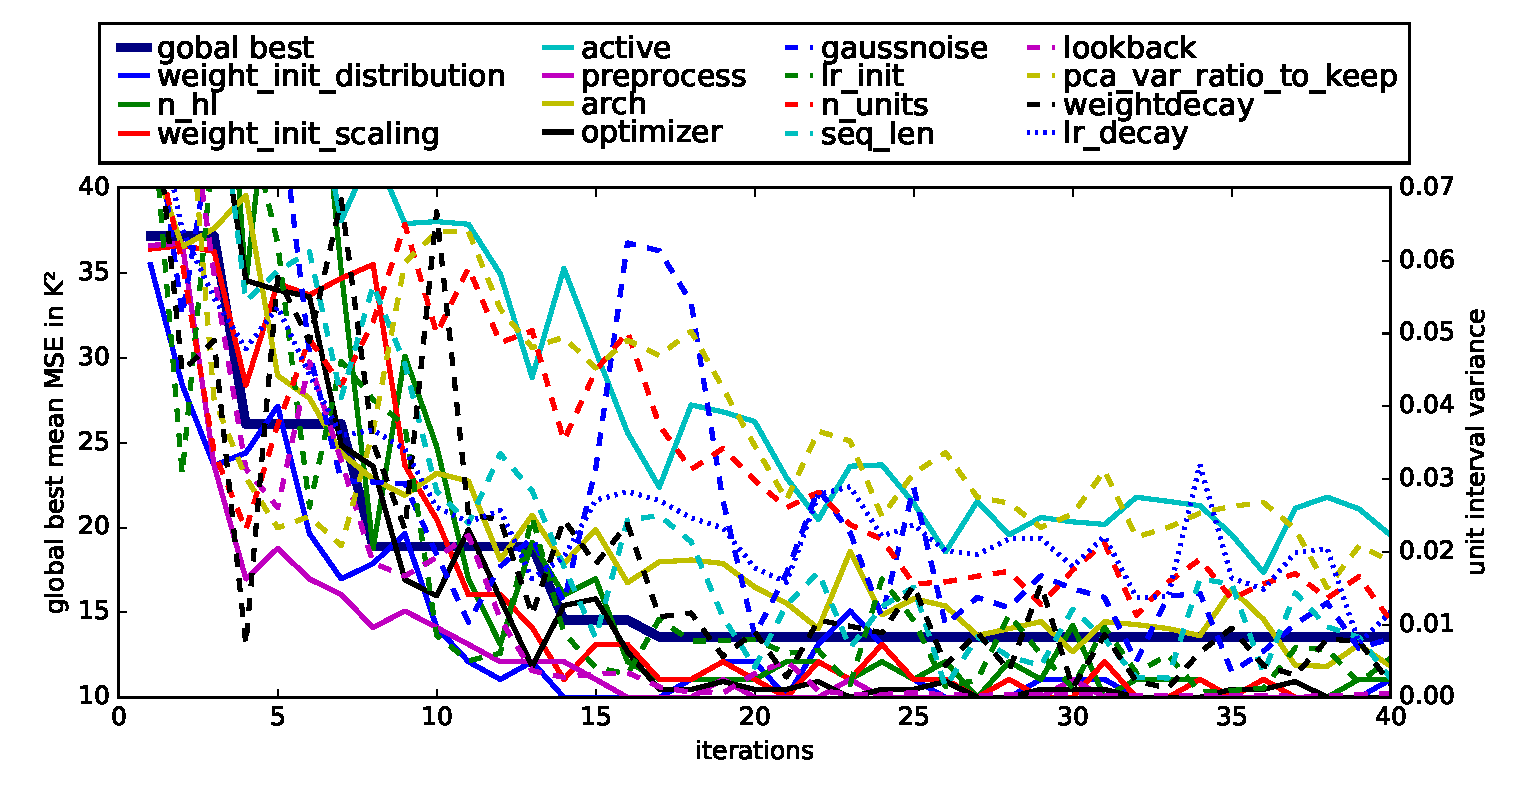
\includegraphics[width=\textwidth]{evaluation/pm_var.eps}
	\caption{Hyper-parameter variance over \gls{pso} iterations (from experiment 3)}
	\label{fig:pm_var}
\end{figure}
\begin{figure}[!hbt]
	\centering
	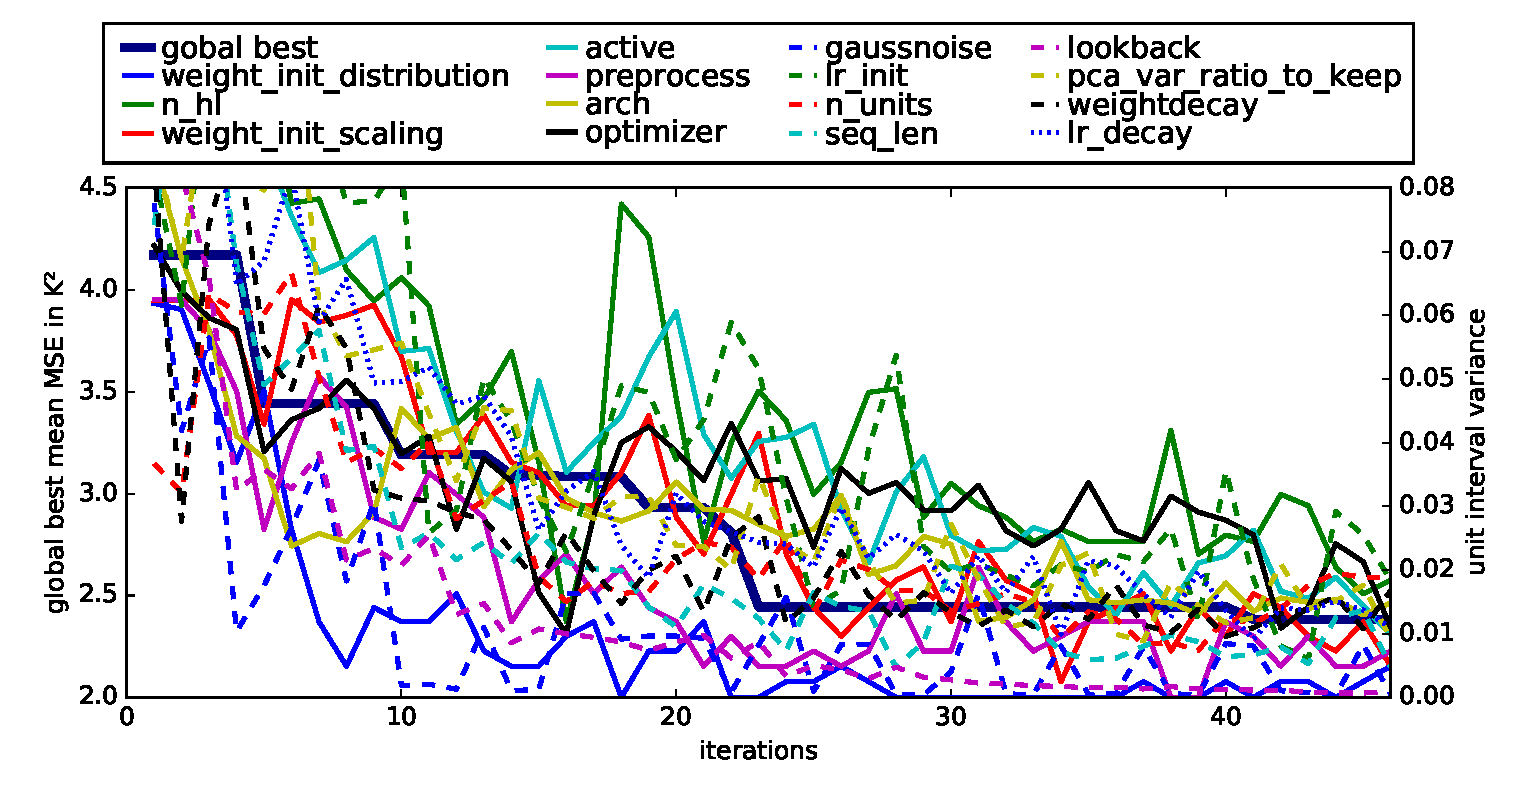
\includegraphics[width=\textwidth]{evaluation/yoke_var.eps}
	\caption{Hyper-parameter variance over \gls{pso} iterations (from experiment 4)}
	\label{fig:yoke_var}
\end{figure}
\begin{figure}[!hbt]
	\centering
	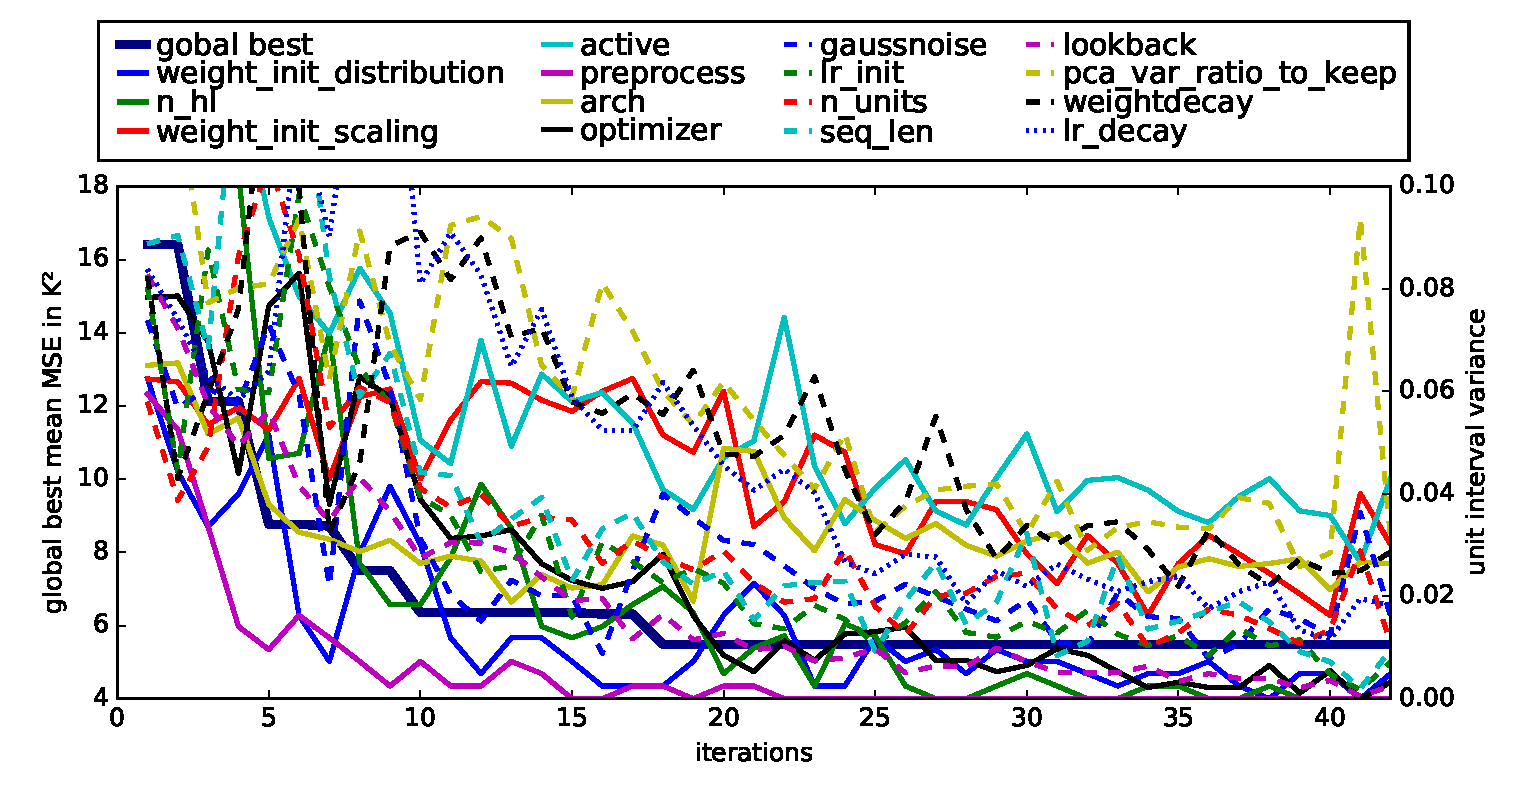
\includegraphics[width=\textwidth]{evaluation/teeth_var.eps}
	\caption{Hyper-parameter variance over \gls{pso} iterations (from experiment 5)}
	\label{fig:teeth_var}
\end{figure}
\begin{figure}[!hbt]
	\centering
	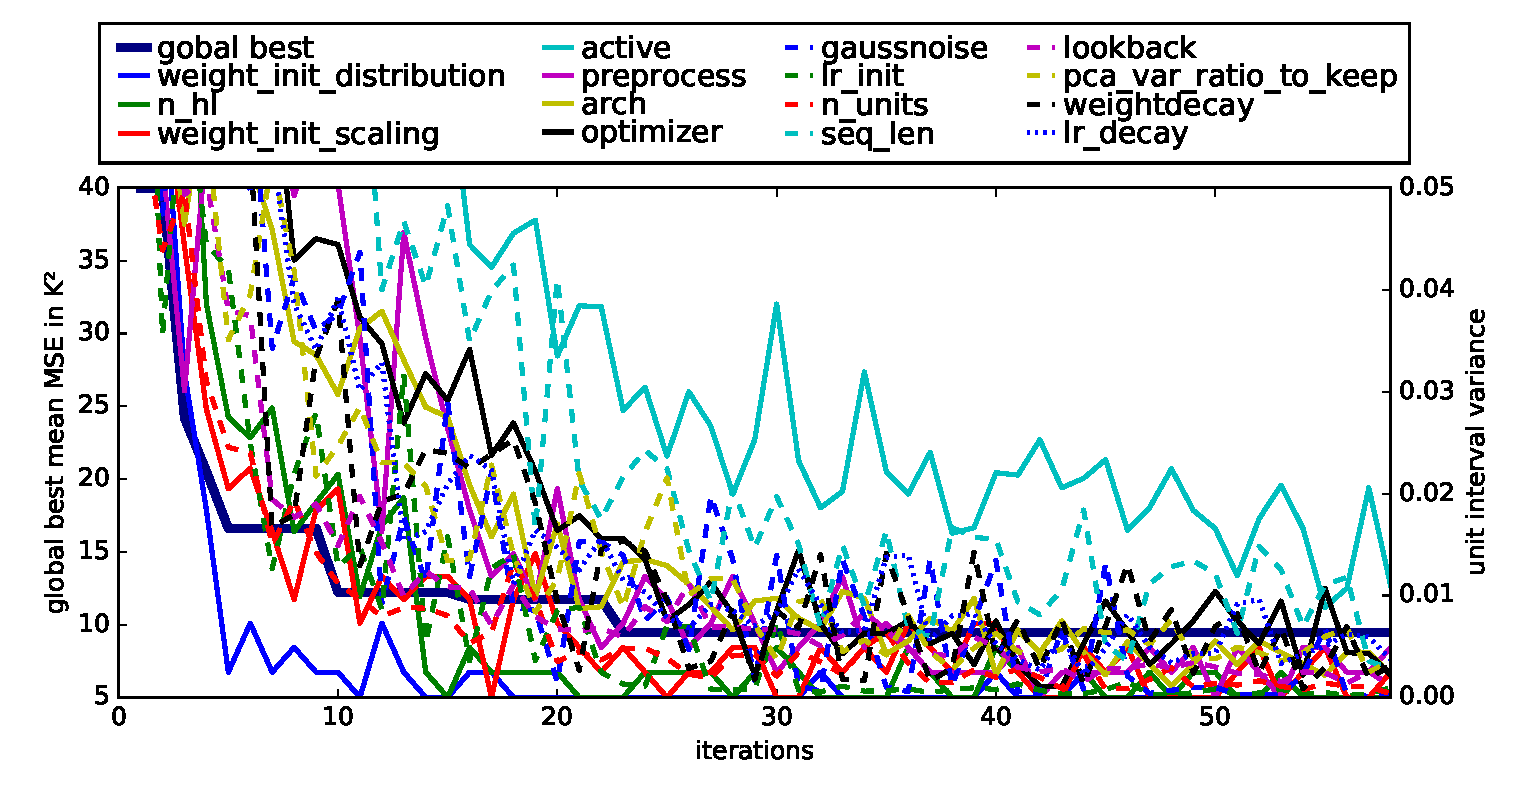
\includegraphics[width=\textwidth]{evaluation/winding_var.eps}
	\caption{Hyper-parameter variance over \gls{pso} iterations (from experiment 6)}
	\label{fig:winding_var}
\end{figure}\clearpage

\section{Sensitivity Analyses}
\label{app:sensitivity}
\begin{table}[h]
	\caption{Sensitivity analysis for experiment 1}
	\label{tab:alltargets_sensitivity}
	\centering
	\begin{tabular}{ C{2.5cm} C{2.5cm} c c}
		\toprule
		\multicolumn{2}{c}{optimum: \SI{33.16}{\kelvin\squared}}&\multicolumn{2}{c}{95\,\% confidence interval: $\pm$ 2.3\,K\textsuperscript{2}}\\
		\midrule
		 hyper-parameter & alternatives & test score estimates in K\textsuperscript{2} & $\Delta$ w.r.t. baseline in K\textsuperscript{2}\\
		 \midrule
		 arch				& \gls{gru}/ \gls{lstm}\_peepholes& 66.79/ 344.84 		& 33.63/ 311.68 \\
		 n\_hl				& 2 							& 124.41 				& 91.25 \\
		 n\_units				& 21/ 57						& 41.93/ 32.66 		& 8.77/ -0.5 \\
		 opt					& \gls{adam}/ \gls{sgd} 			& 59.66/ 40.08 		& 26.5/ 6.92 \\
		 seq\_len				& 7015/ 7880 					& 38.51/ 34.58 		& 5.35/ 1.42\\
		 lookback				& 737/ 1137 					& 40.92/ 35.16 		& 7.76/ 2.0\\
		 lr\_init				&\num{2e-4}					& 37.15				& 3.99\\
		 lr\_decay 			& 0.93/ 0.99					& 40.49/ 34.32			& 7.33/ 1.16\\
		 preprocess 			& \gls{pca}: 0.5/ 1.0				& 248.49/ 50.9			& 215.33/ 17.74\\
		 weight init. distribution& uniform					& 111.23				& 78.07\\
		 weight init. scaling 	& standard 					& 64.17 				& 31.01\\
		 active 				& 0/ 1/ 2 						& 35.41/ 35.88/ 35.02	& 2.25/ 2.72/ 1.86\\
		  \bottomrule
	\end{tabular}
\end{table}

\begin{table}[h]
	\caption{Sensitivity analysis for experiment 2}
	\label{tab:stator_sensitivity}
	\centering
	\begin{tabular}{ C{2.5cm} C{2.5cm} c c}
		\toprule
		\multicolumn{2}{c}{optimum: \SI{12.11}{\kelvin\squared}}&\multicolumn{2}{c}{95\,\% confidence interval: $\pm$ 2.53\,K\textsuperscript{2}}\\
		\midrule
		 hyper-parameter & alternatives & test score estimates in K\textsuperscript{2} & $\Delta$ w.r.t. baseline in K\textsuperscript{2}\\
		 \midrule
		 arch				& \gls{lstm}/ \gls{lstm}+peepholes& 23.5/ 375.24 		& 11.39/ 363.13 \\
		 n\_hl				& 2 							& 222.69 				& 210.58 \\
		 n\_units				& 73/ 201						& 18.25/ 142.47 		& 6.14/ 130.36 \\
		 opt					& nesterov/ \gls{sgd} 			& 42.76/ 17.83 		& 30.65/ 5.72 \\
		 seq\_len				& 6507/ 7880					& 13.74/ 24.97 		& 1.63/ 12.86\\
		 lookback				& 622/ 1022 					& 20.49/ 14.39 		& 8.38/ 2.28\\
		 lr\_init				& \num{8.62e-3}/ \num{3.43e-2}	& 13.31/ 196.85		& 1.2/ 184.74\\
		 lr\_decay 			& 0.92/ 0.99					& 17.31/ 15.22			& 5.2/ 3.11\\
		 preprocess 			& \gls{pca}: 0.5/ 1.0				& 229.96/ 47.64		& 217.85/ 35.53\\
		 weight init. distribution& uniform					& 138.3				& 126.19\\
		 weight init. scaling 	& standard 					& 16.48	 			& 4.37\\
		 active 				& 0/ 2/ 3 						& 13.51/ 14.83/ 18.72	& 1.4/ 2.72/ 6.61\\
		  \bottomrule
	\end{tabular}
\end{table}

\begin{table}[h]
	\caption{Sensitivity analysis for experiment 3}
	\label{tab:pm_sensitivity}
	\centering
	\begin{tabular}{ C{2.5cm} C{2.5cm} c c}
		\toprule
		\multicolumn{2}{c}{optimum: \SI{38.41}{\kelvin\squared}}&\multicolumn{2}{c}{95\,\% confidence interval: $\pm$ 2.98\,K\textsuperscript{2}}\\
		\midrule
		 hyper-parameter & alternatives & test score estimates in K\textsuperscript{2} & $\Delta$ w.r.t. baseline in K\textsuperscript{2}\\
		 \midrule
		 arch				& \gls{lstm}/ \gls{lstm}+peepholes& 47.19/ 183.93 		& 8.78/ 145.52 \\
		 n\_hl				& 2 							& 196.07				& 157.66 \\
		 n\_units				& 86/ 236						& 44.51/ 180.37		& 6.1/ 141.96 \\
		 opt					& nesterov/ \gls{sgd} 			& 85.57/ 66.97			& 47.16/ 28.56  \\
		 seq\_len				& 7095 						& 30.02		 		& -8.21\\
		 lookback				& 1800 						& 40.47		 		& 2.06\\
		 lr\_init				&\num{6.28e-3}/ \num{2.5e-2}	& 78.79/ 219.45		& 40.38/ 181.04\\
		 lr\_decay 			& 0.9/ 0.99					& 41.4/42.88			& 2.99/ 4.47\\
		 preprocess 			& \gls{pca}: 0.5/ 1.0				& 115.6/ 68.96			& 77.19/ 30.55\\
		 weight init. distribution& uniform					& 295.97				& 257.56\\
		 weight init. scaling 	& standard 					& 73.79				& 35.38\\
		 active 				& 0/ 2/ 3						& 39.67/ 38.87/ 38.14	& 1.26/ 0.46/ -0.27\\
		  \bottomrule
	\end{tabular}
\end{table}

\begin{table}[h]
	\caption{Sensitivity analysis for experiment 4}
	\label{tab:yoke_sensitivity}
	\centering
	\begin{tabular}{ C{2.5cm} C{2.5cm} c c}
		\toprule
		\multicolumn{2}{c}{optimum: \SI{7.8}{\kelvin\squared}}&\multicolumn{2}{c}{95\,\% confidence interval: $\pm$ 2.15\,K\textsuperscript{2}}\\
		\midrule
		 hyper-parameter & alternatives & test score estimates in K\textsuperscript{2} & $\Delta$ w.r.t. baseline in K\textsuperscript{2}\\
		 \midrule
		 arch				& \gls{lstm}/ \gls{lstm}+peepholes& 28.17/ 265.32 		& 20.37/ 257.52 \\
		 n\_hl				& 2 							& 98.57 				& 90.77 \\
		 n\_units				& 142/ 300					& 6.86/ 17.64 			& -0.94/ 9.84 \\
		 opt					& nesterov/ \gls{sgd} 			& 14.79/ 8.95 			& 6.99/ 1.15  \\
		 seq\_len				& 77/ 1647 					& 12.38/ 29.35 		& 4.58/ 21.55\\
		 lookback				& 860/ 1260 					& 7.36/ 6.3	 		& -0.44/ -1.5\\
		 lr\_init				&\num{5.65e-3}/ \num{2.25e-2}	& 6.78/ 103.95			& -1.02/ 96.15\\
		 lr\_decay 			& 0.85/ 0.95					& 6.17/ 5.75			& -1.63/ -2.05\\
		 preprocess 			& \gls{pca}: 0.5/ 1.0				& 353.53/ 81.3			& 345.73/ 73.5\\
		 weight init. distribution& uniform					& inf.				& inf.\\
		 weight init. scaling 	& normalized 					& 49.18 				& 41.38\\
		 active 				& 0/ 1/ 3						& 5.64/ 15.10/ 7.84		& -2.16/ 7.3/ 0.04\\
		  \bottomrule
	\end{tabular}
\end{table}

\begin{table}[h]
	\caption{Sensitivity analysis for experiment 5}
	\label{tab:teeth_sensitivity}
	\centering
	\begin{tabular}{ C{2.5cm} C{2.5cm} c c}
		\toprule
		\multicolumn{2}{c}{optimum: \SI{12.41}{\kelvin\squared}}&\multicolumn{2}{c}{95\,\% confidence interval: $\pm$ 2.22\,K\textsuperscript{2}}\\
		\midrule
		 hyper-parameter & alternatives & test score estimates in K\textsuperscript{2} & $\Delta$ w.r.t. baseline in K\textsuperscript{2}\\
		 \midrule
		 arch				& \gls{lstm}/ \gls{lstm}+peepholes& 24.63/ 260.72		&  12.22/ 248.31\\
		 n\_hl				& 2 							& 18.23				& 5.82 \\
		 n\_units				& 69/ 189						& 14.88/ 12.66			& 2.47/ 0.25 \\
		 opt					& nesterov/ \gls{sgd} 			& 17.15/ 19.3 			& 4.74/ 6.89  \\
		 seq\_len				& 30/ 1145 					& 18.84/ 20.01 		& 6.43/ 7.6\\
		 lookback				& 680/ 1080 					& 19.35/ 14.24 		& 6.94/ 1.83\\
		 lr\_init				&\num{1.1e-3}/ \num{4.39e-3}	& 15.91/ 17.68			& 3.5/ 5.27\\
		 lr\_decay 			& 0.74/ 0.84					& 17.73/ 16.42			& 5.32/ 4.01\\
		 preprocess 			& \gls{pca}: 0.5/ 1.0				& 340.34/ 189.23		& 327.93/ 176.82\\
		 weight init. distribution& uniform					& inf.				& inf.\\
		 weight init. scaling 	& normalized 					& 21.92				& 9.51\\
		 active 				& 0/ 1/ 3						& 20.89/ 16.0/ 14.12	& 8.48/ 3.59/ 1.71\\
		  \bottomrule
	\end{tabular}
\end{table}

\begin{table}[h]
	\caption{Sensitivity analysis for experiment 6}
	\label{tab:winding_sensitivity}
	\centering
	\begin{tabular}{ C{2.5cm} C{2.5cm} c c}
		\toprule
		\multicolumn{2}{c}{optimum: \SI{21.53}{\kelvin\squared}}&\multicolumn{2}{c}{95\,\% confidence interval: $\pm$ 2.82\,K\textsuperscript{2}}\\
		\midrule
		 hyper-parameter & alternatives & test score estimates in K\textsuperscript{2} & $\Delta$ w.r.t. baseline in K\textsuperscript{2}\\
		 \midrule
		 arch				& \gls{lstm}/ \gls{lstm}+peepholes& 61.96/ 469.27		& 40.43/ 447.74\\
		 n\_hl				& 2 							& 38.37				& 16.84 \\
		 n\_units				& 23/ 62						& 29.05/ 18.85			& 7.85/ -2.68\\
		 opt					& nesterov/ \gls{sgd} 			& 41.41/ 41.13			& 6.94/ 19.6\\
		 seq\_len				& 5885/ 7455 					& 28.47/ 26.24 		& 6.94/ 4.71\\
		 lookback				& 532/932 					& 28.27/ 22.94 		& 6.74/ 1.41\\
		 lr\_init				&\num{1.09e-2}/ \num{4.33e-2}	& 25.64/ 44.89			& 4.11/ 23.36\\
		 lr\_decay 			& 0.61/ 0.7					& 23.0/ 20.86			& 1.47/ -0.67\\
		 preprocess 			& \gls{pca}: 0.5/ 1.0				& 262.79/ 589.68		& 241.26/ 568.15\\
		 weight init. distribution& uniform					& 115.64				& 94.11\\
		 weight init. scaling 	& standard 					& 46.45				& 24.92\\
		 active 				& 0/ 1/ 3						& 24.16/ 20.30/ 21.01	& 2.63/ -1.23/ -0.52\\
		  \bottomrule
	\end{tabular}
\end{table}


    
    \backmatter
    \titleformat{\chapter}
    [display] % The paragraph shape
    {\bfseries\huge} % Format of the main text
    {} % Label is ommitted here, since it is below
    {0ex}
    {\vspace{-5ex}\titlerule\vspace{1.5ex}\filright~}
    [\vspace{1ex}\titlerule]
    
    \chapter{Symbols}
\label{chapter:symbols}

\begin{flushleft}
	\rarray{1.3}
  \begin{longtable}{L{4.2cm}L{11.3cm}}
  $\alpha$ & Decay rate\\
  $\alpha_d$ & Learning rate decay factor\\
  $\delta_k$ & Sensitivity of output neuron $k$\\
  $\epsilon$ & Weight init. scaling factor\\
  $\eta$ & Learning rate or step size\\
  $\vartheta_a$ & Ambient temperature\\
  $\vartheta_c$ & Liquid coolant temperature\\
  $\vartheta_{PM}$ & Permanent magnet temperature\\
  $\vartheta_{SY}$ & Stator yoke temperature\\
  $\vartheta_{ST}$ & Stator Teeth temperature\\
  $\vartheta_{SW}$ & Stator Winding temperature\\
  $\lambda$ & Weight decay penalty factor\\
  $\mu$ & Sample mean or momentum rate\\
  $\sigma$ & Sample standard deviation or sigmoid activation function\\
   $\phi$ & Tanh activation function\\
  $\Psi_p$ & Permanent magnet flux linkage\\
  $\omega_{el}$ & Electrical angular velocity\\
  $\omega_{mech}$ & Mechanical angular velocity\\
  $a_j$ & Net activation of the neuron $j$\\
  $\bm b_h$ & Bias vector to the activations in layer $h$\\
  $b_j$ & Real-valued bias to the activation of node $j$\\
  $c_{max}$ & Maximum confidence in best found positions\\
  $c_{self}$ & Constant inertia for a particle's displacement\\
  $f$ & Forget gate\\
  $f_i$ & Fan-in\\
   $f_o$ & Fan-out\\
   $g$ & Block input\\ 
   $g_i$ & Global best value for a certain particle's $i$-th dimension\\
   $g_{thresh}$ & Gradient clipping threshold\\
   $\bm h$ & Output vector of a whole layer\\
   $\tilde h$ & Block input for \gls{gru}\\
   $i$ & Input gate \\
   $I$ & Current amplitude\\
   $i_d$ & Actual current $d$-axis component (measured)\\
   $i_q$ & Actual current $q$-axis component (measured)\\
   $i_{sd}$ & Current on the $d$-axis \\
   $i_{sq}$ & Current on the $q$-axis \\
   $\mathcal L$ & Cost function\\
   $l_j$ & Activation function at neuron $j$\\
   $l_h$ & Activation function of each neuron within layer $h$\\
   $L_s$ & Self inductance\\
   $l_2$ & Accumulated L2-norm of the gradient vector\\
   $n_{mech}$ & Motor speed\\
   $o$ & Output gate\\
   $p$ & Pole pair number\\
   $\bm p$ & Peephole weight vector\\
   $p_i$ & Personal best value for a certain particle's $i$-th dimension\\
   $r$ & Reset gate\\
   $R_s$ & Stator resistance\\
   $s_c$ & Internal cell state\\
   $T$ & Torque\\
   $T_n$ & Delay time\\
   $T_x$ & Actual torque (measured)\\
   $u$ & Realization of a uniformly distributed random variable between 0 and 1\\
   $U$ & Voltage amplitude\\
   $u_{sd}$ & Voltage on the $d$-axis  \\
   $u_{sq}$ & Voltage on the $q$-axis  \\
   $u_d$ & Actual voltage $d$-axis component (measured)\\
   $u_q$ & Actual voltage $q$-axis component (measured)\\
   $\bm v$ & Gradient velocity\\
   $v_i$ & Velocity of the $i$-th particle dimension\\
   $v_j$ & Real-valued output of a node $j$\\      
   $\bm w$ & The weight matrix unraveled to a weight vector\\
   $\bm W^{hh'}$ & Weight matrix assigned to the edges from layer $h'$ to $h$\\
   $w_{jj'}$ & Real-valued weight assigned to the edge from node $j'$ to node $j$\\
   $\bm x^{(t)}$ & Input vector at time $t$\\
   $\bm y^{(t)}$ & Target vector at time $t$\\
   $\bm{\hat y}^(t)$ & Predicted output vector at time $t$\\
   $z$ & Update gate\\
  \end{longtable}
\end{flushleft}

    
    \listoffigures
    \listoftables
    
    \printglossaries
    
    \printbibliography
\end{document}
